\documentclass[8pt, a4paper, landscape, fleqn]{scrartcl}
\usepackage[utf8]{inputenc}
\usepackage[ngerman]{babel}

\usepackage{hyperref}

%Layout
\usepackage{multicol, geometry, xcolor}
\geometry{margin=1cm}
\parindent 0pt
\pagestyle{empty}

\newlength{\breite}
\setlength{\breite}{0.5pt}
\setlength{\columnseprule}{\breite}

\usepackage{graphicx}
\usepackage{tikz}


%Mathematik-Pakete
\usepackage{amsmath, amstext, amssymb, mathtools, esint, polynom}
\usepackage{bm}
\usepackage{esvect}
\allowdisplaybreaks %Seitenumbruch in align-Umgebung erlauben


% define some colors
\definecolor{section}{RGB}{150,101,203}
\definecolor{subsection}{RGB}{178,166,216}
\definecolor{subsubsection}{RGB}{209,201,232}
\definecolor{titletext}{RGB}{0,0,0}

% section color box
\setkomafont{section}{\mysection}
\newcommand{\mysection}[1]{%
	\Large\sf%
	\setlength{\fboxsep}{0cm}%already boxed
	\colorbox{section}{%
		\begin{minipage}{\linewidth}%
			\vspace*{2pt}%Space before
			\leftskip2pt %Space left
			\rightskip\leftskip %Space right
			{\color{titletext} #1}
			\vspace*{1pt}%Space after
		\end{minipage}%
}}
% subsection color box
\setkomafont{subsection}{\mysubsection}
\newcommand{\mysubsection}[1]{%
	\Large\sf%
	\setlength{\fboxsep}{0cm}%already boxed
	\colorbox{subsection}{%
		\begin{minipage}{\linewidth}%
			\vspace*{2pt}%Space before
			\leftskip2pt %Space left
			\rightskip\leftskip %Space right
			{\color{titletext} #1}
			\vspace*{1pt}%Space after
		\end{minipage}%
}}

% subsubsection color box
\setkomafont{subsubsection}{\mysubsubsection}
\newcommand{\mysubsubsection}[1]{%
	\sf%
	\setlength{\fboxsep}{0cm}%already boxed
	\colorbox{subsubsection}{%
		\begin{minipage}{\linewidth}%
			\vspace*{1pt}%Space before
			\leftskip2pt %Space left
			\rightskip\leftskip %Space right
			{\color{titletext} #1}
			\vspace*{1pt}%Space after
		\end{minipage}%
}}

				
\providecommand{\diff}{\mathop{} \! \mathrm{d}}




\title{Lineare Algebra Einführung}
\subtitle{HS 2023 Prof. Dr. Andreas Müller}
\author{Fabian Suter, \today}
\date{{\small \url{https://github.com/FabianSuter/LinAlg}}}
 
 
\begin{document}
	\begin{multicols*}{3}
	
		\maketitle
		
		\section{Lineare Gleichungssysteme}
		    \subsection{Matritzen und Vektoren}
			Matrix: $A = \begin{pmatrix}
				6&1&2\\
				5&4&0\\
				4&1&9
			\end{pmatrix}$ \qquad
			Einheitsmatrix: $E = \begin{pmatrix}
				1&0&0\\
				0&1&0\\
				0&0&1
			\end{pmatrix}$ \\
			\\
			Zeilenvektor: $a = \begin{pmatrix}
a_1&a_2&a_n \end{pmatrix}$ \quad Spaltenvektor: $b =  \begin{pmatrix} 1\\2\\3 \end{pmatrix}$ 	\\
			
			Standardbasisvektoren:  $ e_1=\begin{pmatrix}1\\0\\0\end{pmatrix},
\qquad
e_2=\begin{pmatrix}0\\1\\0\end{pmatrix},
\qquad
e_3=\begin{pmatrix}0\\0\\1\end{pmatrix}$ \\
	
				
			\subsection{Rechenregeln mit Matritzen und Vektoren}
		    \subsubsection{Addition / Subtraktion}
			Beschreibung für Spaltenvektoren $\rightarrow$ gilt analog für Zeilenvektoren! \\
			Beschreibung nur für Addition $\rightarrow$ gilt analog für Subtraktion! \\

			$a = \begin{pmatrix} 1\\2\\3 \end{pmatrix}$ \quad $b = \begin{pmatrix} 4\\5\\6 \end{pmatrix}$ \quad  $a+b = \begin{pmatrix} 1+4\\2+5\\3+6 \end{pmatrix}$ \\
			\\
			$A=\begin{pmatrix}
				1&2\\
				3&4\\
				5&6
			\end{pmatrix}$ \quad $ B=\begin{pmatrix}
				0&7\\
				5&3\\
				6&2
			\end{pmatrix}$ \quad $A+B=\begin{pmatrix}
				1+0&2+7\\
				3+5&4+3\\
				5+6&6+2
			\end{pmatrix}$

		    
			\subsubsection{Multiplikation}
			% Vektor mal Faktor
			$v = \begin{pmatrix} 1\\8\\4 \end{pmatrix}$ \qquad $\lambda \cdot v = \begin{pmatrix} \lambda \cdot 1\\\lambda \cdot 8\\\lambda \cdot 4 \end{pmatrix}$ \\
			\\
			
			%Matrix mal Faktor 
			$D=\begin{pmatrix}
				6&1&2\\
				5&4&0\\
				4&1&9
			\end{pmatrix}$ \qquad $\lambda \cdot 				D=\begin{pmatrix}
				\lambda \cdot 6 & \lambda \cdot 1 & \lambda \cdot 2 \\
				\lambda \cdot 5 & \lambda \cdot 4 & \lambda \cdot 0\\
				\lambda \cdot 4 & \lambda \cdot 1 & \lambda \cdot 9
			\end{pmatrix}$ \\
			\\
				
			% Matrix mal Vektor			

$D \cdot v = \begin{pmatrix}
\color{red}6&\color{red}1&\color{red}2\\
5&4&0\\
4&1&9
\end{pmatrix}
\begin{pmatrix}
\color{blue}1\\\color{blue}8\\\color{blue}4
\end{pmatrix}
=
\begin{pmatrix}
{\color{red}6}\cdot{\color{blue}1}+
{\color{red}1}\cdot{\color{blue}8}+
{\color{red}2}\cdot{\color{blue}4}
\\
5\cdot{\color{blue}1}+
4\cdot{\color{blue}8}+
0\cdot{\color{blue}4}
\\
4\cdot{\color{blue}1}+
1\cdot{\color{blue}8}+
9\cdot{\color{blue}4}
\end{pmatrix}
=\begin{pmatrix}
22\\37\\48
\end{pmatrix}$ \\
\\


			% Matrix mal Matrix
			$A=\begin{pmatrix}
\color{red}1&\color{red}2&\color{red}4\\
0&4&-1
\end{pmatrix}$, \qquad 
$B =\begin{pmatrix}
\color{blue}-2&4\\
\color{blue}-4&-5\\
\color{blue}2&4
\end{pmatrix}
\\
\\
A \cdot B =
\begin{pmatrix}
{\color{red}1}\cdot({\color{blue}-2})+{\color{red}2}\cdot({\color{blue}-4})+{\color{red}4}\cdot{\color{blue}2} &
{\color{red}1}\cdot 4+{\color{red}2}\cdot(-5)+{\color{red}4}\cdot 4\\
0\cdot ({\color{blue}-2})+4\cdot({\color{blue}-4})+(-1)\cdot {\color{blue}2} &
0\cdot 4+4\cdot(-5)+(-1)\cdot 4
\end{pmatrix}$ \\


			\subsubsection{Division}
			Divisionen von Matritzen werden durch eine Multiplikation mit der inversen Matrix durchgeführt.

   			\subsubsection{Zusammenfassung / Erweiterung der Rechenregeln}
   			\begin{tabular}{lll}
   			Symmetrie: & $ A = A^t$ \\   			
   			Orthagonalität: &  $ A A^t = A^t A = E $  & $A^{-1} = A^t$\\
   			& $A^t$ auch orthagonal & $\det(A) = \pm 1$ \\
   			Produkte: & \textbf{AB $\neq$ BA} & $(AB)C = A(BC)$\\
   			& $EA = A = AE$  & $A(B + C) = AB + AC$\\
   			& $A (\lambda B) = (\lambda A) B$ & \\
   			Transponiert: & $(AB)^t = B^t A^t $ \\
   			Inverse: & $A^{-1} A = E$ & $(AB)^{-1} = B^{-1} A^{-1} $ \\
   			Potenzen: & $(A^t)^{-1} = (A^{-1})^t $ & $Ax = b, x = A^{-1}b$\\
   			\end{tabular}
		    
		    
		    \subsection{Transponierte Matrix $A^t$}
		    Spiegelung an Diagonalen \\
		    \\
		    $A=\begin{pmatrix}
				a&b&c\\
				d&e&f\\
				g&h&i
			\end{pmatrix}$ \quad $ A^T =\begin{pmatrix}
				a&d&g\\
				b&e&h\\
				c&f&i
			\end{pmatrix}$    
		        
		        
		    \subsection{Inverse Matrix $A^{-1}$}
		    Die Inverse Matrix ist \textbf{nur für quadratische Matritzen} definiert.
		    Die Inverse Matrix kann durch dar Gauss-Verfahren oder mit dem Entwicklungssatz berechnet werden. \\
		    \\
		    1. Gauss: \quad $A^{-1}$ \quad \begin{tabular}{|c|c|}
		    					\hline
		    					A & E \\
		    					\hline
		    					\end{tabular} \quad $\underrightarrow{\text{Gauss}}$ \quad \begin{tabular}{|c|c|}
		    					\hline
		    					E & $A^{-1}$ \\
		    					\hline
		    					\end{tabular} \\
					\\
			2. Entwicklungssatz: \quad $A^{-1} = \frac{1}{\det(A)} \cdot \mathrm{adj}(A) $  für $\det(A) \neq 0$ \\
			\\
			Bsp. 2 x 2 Matritzen: \quad $A^{-1} = \frac{1}{ad-bc} \cdot \begin{pmatrix}
			d & -b \\
			-c & a 
			\end{pmatrix} $  für $\det(A) \neq 0$ \\
			\\
			\textbf{$\rightarrow$ für Variante Entwicklungssatz siehe Beispiel nächste Seite} \\
			

			\subsection{Lineares Gleichungssystem }
			 Ein Lineares Gleichungssystem kann als Matrix geschrieben werden:
			 
			 \textbf{Beispiel}\\
			 \begin{tabular}{llllll |c c | c|}
			 $x$ & + & $3 \, y$ & = & $1$  \\
			 $-x$ & + & $5 \, y$ & = & $-1$  \\
			 \end{tabular} 
			\\
			 
			Das Gleichungssystem wird in eine Matrix abgefüllt: \\
			\\
			 \begin{tabular}[h]{|c c | c|}
			 \hline
			 $x$ & $y$ & $b$\\
			 \hline
			 $1$ & $3$ & $1$ \\
			 $-1$ & $5$ & $-1$ \\
			 \hline
			 \end{tabular}
			 
			 
			 \subsubsection{Lineare Gleichungssysteme lösen}
			 \begin{tabular}{ll}
			 $\bullet$ & Gauss-Algorithmus \\
			 $\bullet$ & Inverse Matrix $x = A^{-1} \cdot b$ \\
			 $\bullet$ & Cramersche Regel \\
			 \end{tabular}
			 
			 
		    \subsection{Gauss-Algorithmus}
		    Die aktuelle Zeile wird durch das \textcolor{red}{Pivot-Element} ($\neq 0$) geteilt. \\  
		     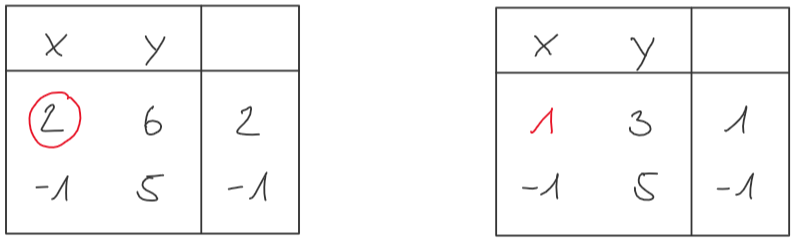
\includegraphics[width=0.45\linewidth]{Bilder/gauss1} \\
		   	

		    Anschliessend werden alle Spalten unterhalb des Pivots auf \textcolor{blue}0 gesetzt, indem man das x-Fache der neuen "Pivot- Zeile" von der entsprechenden Zeile subtrahiert / addiert. \\
		    \\
		    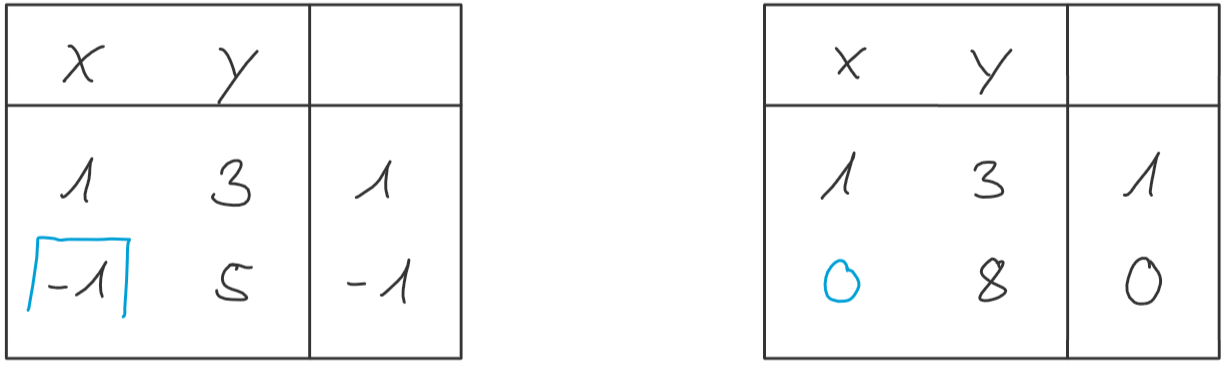
\includegraphics[width=0.45\linewidth]{Bilder/gauss2} \\
		    \\
		    Schritt 1 und Schritt 2 wiederholen, bis nur noch 1en auf der Diagonalen stehen. \\
		    \\
		    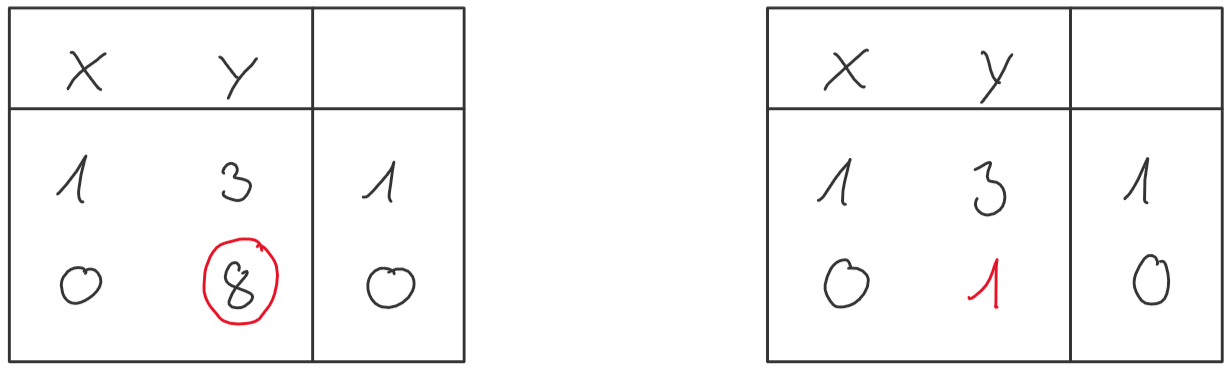
\includegraphics[width=0.45\linewidth]{Bilder/gauss3} \\
		    \\
		    Wenn nur noch 1en auf der Diagonale stehen muss nur doch die blaue Operation durchgeführt werden (Rückwärts-Einsetzen) \\
		    \\
		    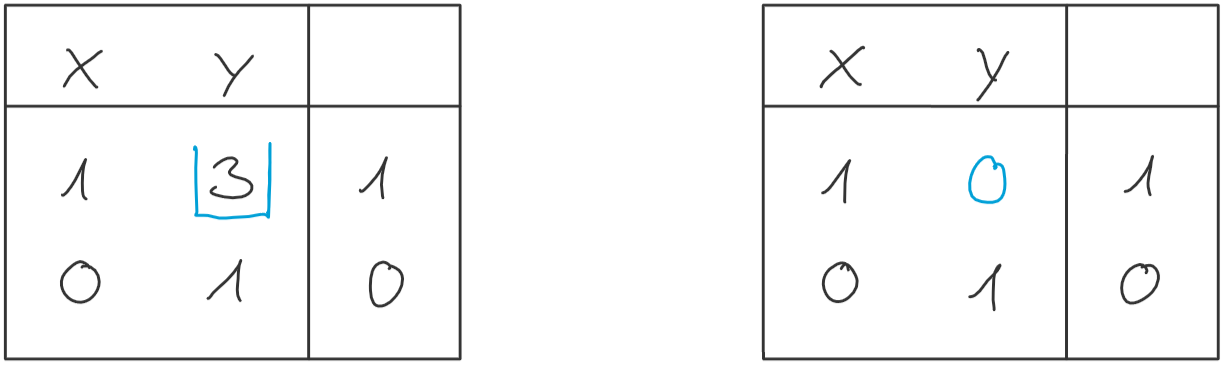
\includegraphics[width=0.45\linewidth]{Bilder/gauss4} \\
		    
		    
		    
			\subsubsection{Spezialfall RREF}
	
			\begin{minipage}[b]{.5\linewidth} 
  			\includegraphics[width=\linewidth]{Bilder/RREF-Tableau}
			\end{minipage}
			\hfill
			\begin{minipage}[b]{.45\linewidth} 
  			Wenn die nächste Spalte im Gauss-Algorithmus kein Pivot-Element enthält (0 ist), kann die Spalte 						übersprungen werden. Die Spalte repräsentiert eine 					\textcolor{green}{frei wählbare Variable} \\
			$\rightarrow$ Siehe Abschnitt zu Lösungsmenge\\	
			\end{minipage}			
   		
   			
   			
   			
   		
   		
   		
   		
		    \subsubsection{Simultane Lösung (mehrere Rechte Seiten)}
		    Wenn zwei Gleichungssysteme sich nur auf der rechten Seite \\
		    unterscheiden können sie in das gleiche Gauss-Tableau abgefüllt werden.\\
		    $\rightarrow$ normal mit Gauss-Algorithmus lösen \\
		    \\
		    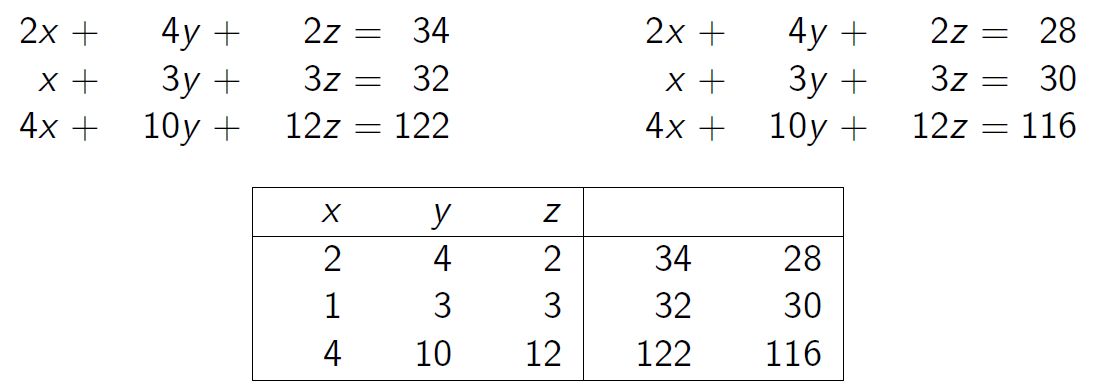
\includegraphics[width=0.6\linewidth]{Bilder/mehrere_rechte_seiten}
		    
		    
		    \subsection{Lösungsmenge}
		    	Falls mehr Unbekannte als Gleichungen vorhanden sind, können nicht alle Unbekannten bestimmt werden. \\
		    	

		 	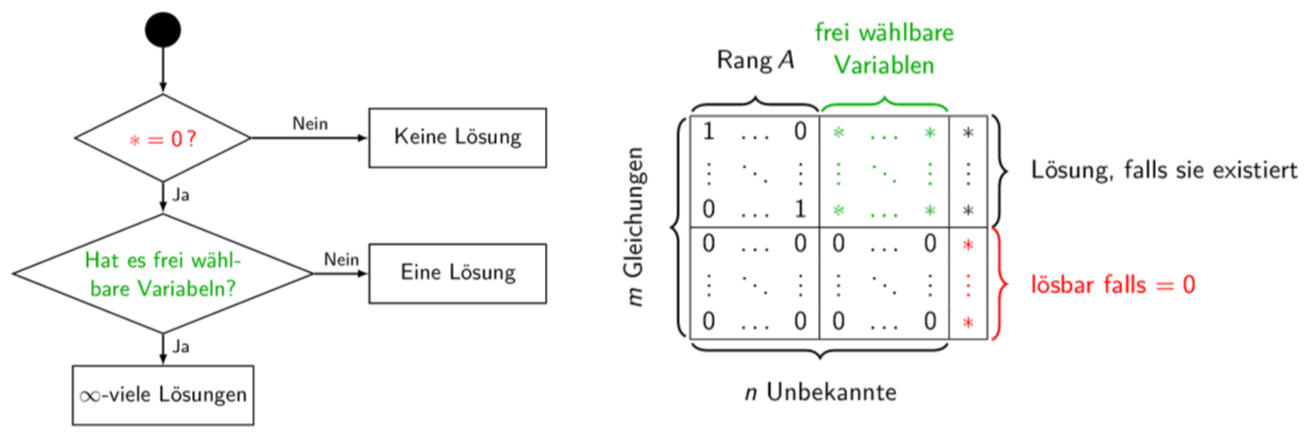
\includegraphics[width=0.9\linewidth]{Bilder/entscheidungsbaum} 	\\
			 \\
			 Wenn es unendlich viele Lösungen gibt kann die Lösungsmenge folgendermassen angegeben werden \\
			 \textbf{Vorzeichenwechsel bei frei wählbaren Variablen beachten!}\\
			 \\
			  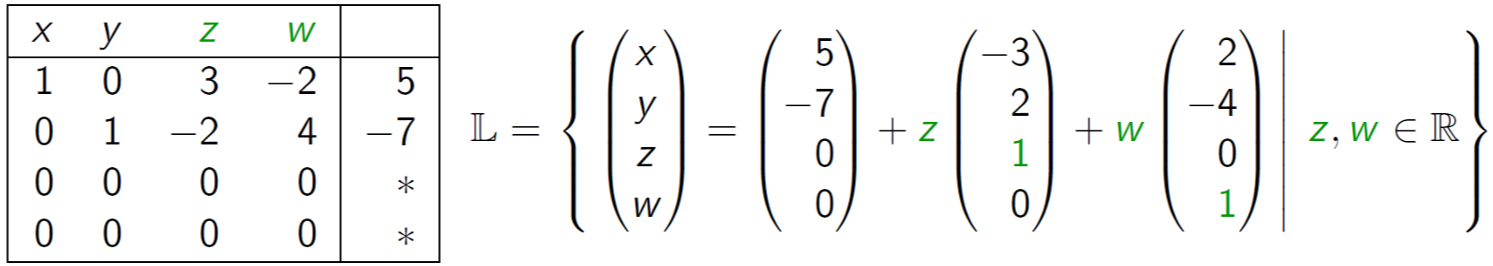
\includegraphics[width=0.9\linewidth]{Bilder/loesungsmenge-gauss-tableau} \\
				  
		    
		    \subsection{Rang einer Matrix}
			Anzahl linear unabhängiger Zeilen / Spalten \\		    
		    Entspricht der Anzahl eindeutig bestimmbarer Variablen \\
		    
		    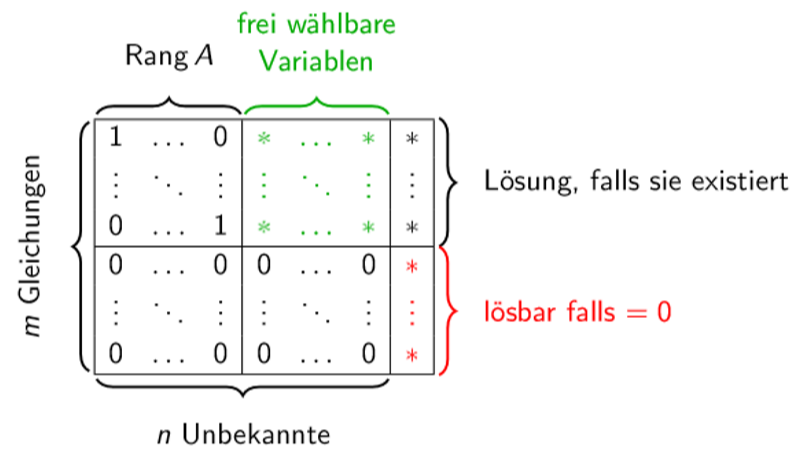
\includegraphics[width=0.7\linewidth]{Bilder/loesungsmenge-gauss}
		    
			
			
					    
		    
		    
		    
		    \subsection{Lineare Abhängigkeit}
		    Wenn eine Zeile ein Vielfaches einer anderen Zeile ist, sind die Zeilen linar abhängig. \\
		    Beim Gauss-Algorithmus entsteht eine Nullzeile. \\
		    \\
		    $\lambda_1 \cdot$ Zeile 1 + $\lambda_2 \cdot$ Zeile 2 + $\lambda_3 \cdot$ Zeile 3 = Nullzeile \\
		    \\
		    Um die Koeffizienten $\lambda_i$ zu finden wird dir ursprüngliche \\
		    Matrix A transponiert und auf Null gesetzt. \\
		    \\
		    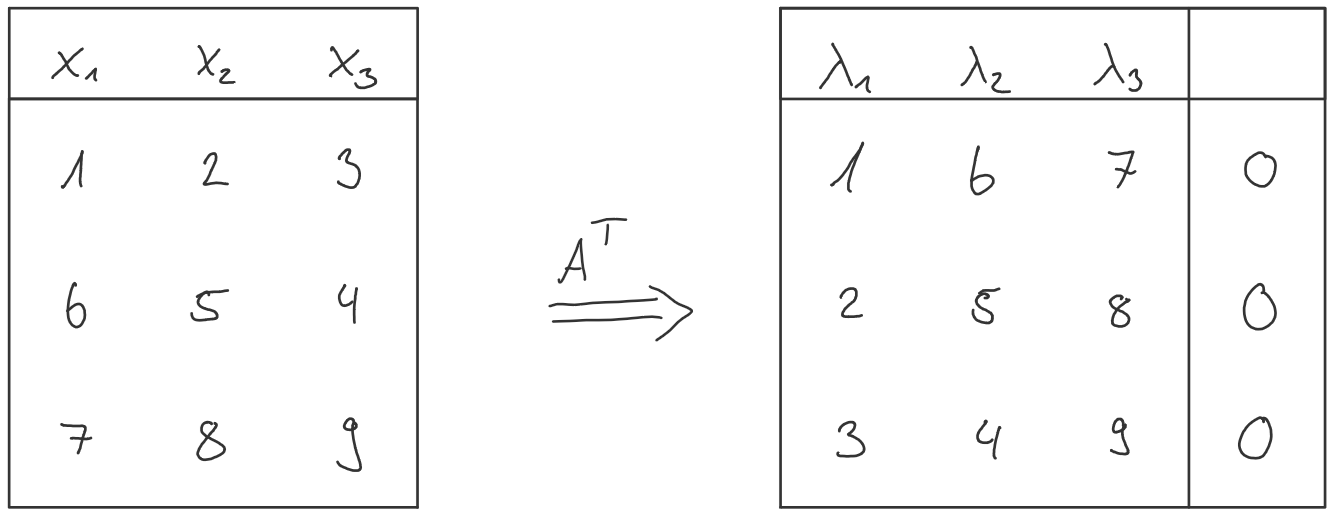
\includegraphics[width=0.5\linewidth]{Bilder/lineare-abhaengigkeit_1} \\
		    \\
		    Die neue Matrix wird mit dem Gauss-Verfahren gelöst\\
		    
		    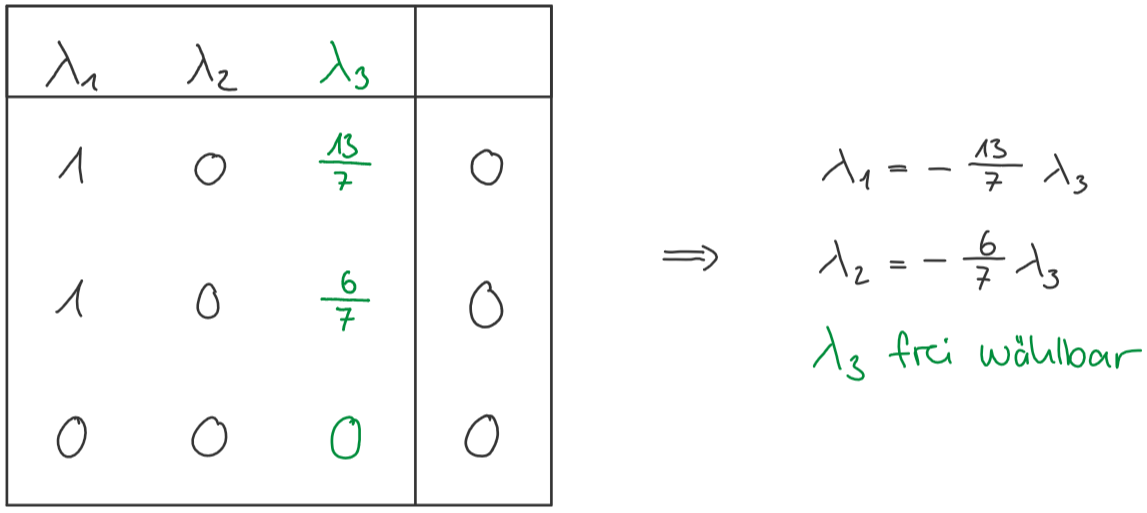
\includegraphics[width=0.5\linewidth]{Bilder/lineare-abhaengigkeit_2} \\
		    
		    
		    
			\subsection{Lineares Gleichungssystem $A \cdot x = b$}	
			Ein lineares Gleichungssystem entstspricht dem Produkt aus Matrix mal Vektor \\
			\\
			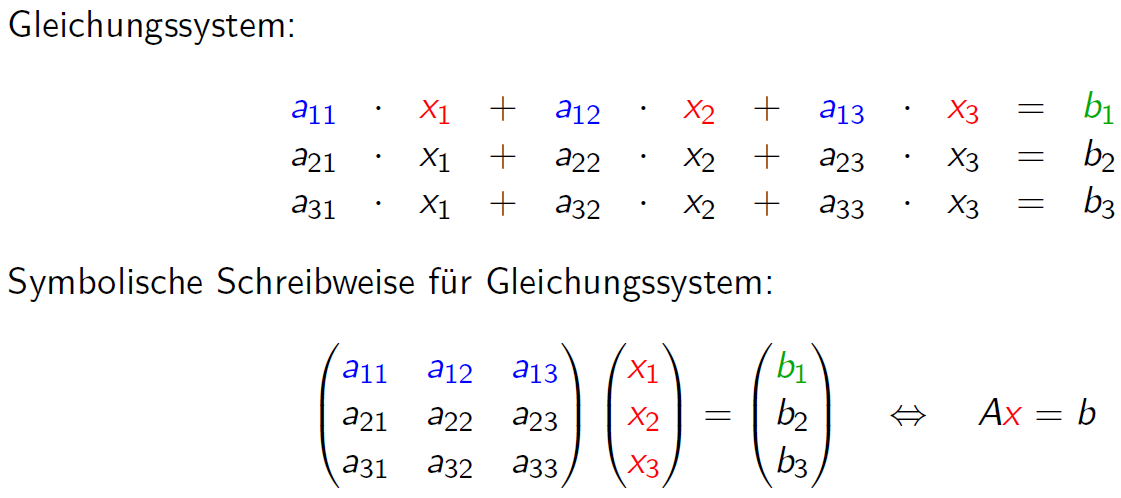
\includegraphics[width=0.8\linewidth]{Bilder/Ax_b} \\
			\\
			Dieses Gleichungssystem bestitz die Lösung $x = A^{-1} \cdot b$ \\	
				    
		    
		    
		    \subsection{Homogene / Inhomogene LGS}
		    \begin{tabular}{ll}
		    Inhomogen: & $Ax = b$ \\
		    Homogen: & $Ax = 0$ \\
		    \end{tabular}
		    
		    
		    
		    \subsection{Reguläre / Singuläre Matrix}
		    Die Begriffe sind nur für quadratische Matritzen definiert! \\
		    \begin{tabular}{lll}
		    regulär: & genau 1 Lösung & $\rightarrow$ det(A) $\neq$ 0 \\
		    singulär: & 0 oder $\infty$ Lösungen & $\rightarrow$ det(A) = 0 \\
		    \end{tabular}
		    
		    
		 \section{Determinante}
		 Die Determinante ist eine Kennzahl dafür, ob eine \textbf{quadratische} Matrix singulär oder regulär ist. \\
		 \\
		  \begin{tabular}{ll}
		    regulär: & $\det(A) \neq 0$ \\
		    singulär: & $ \det(A) = 0$ \\
		  \end{tabular}
		    
		    \subsection{Notation}
		     $A = \begin{bmatrix}
		    			a & b & c \\
		    			d & e & f \\
		    			g & h & i 
		    		\end{bmatrix}$  \qquad  $\det(A) = \begin{vmatrix}
		    			a & b & c \\
		    			d & e & f \\
		    			g & h & i 
		    			\end{vmatrix}$ \\
		    
		    
		    \subsection{Definierende Eigenschaften der Determinante}
		    \begin{tabular}{ll}
		    1. & Wenn eine Zeile mit einem Faktor $\lambda$ multipliziert wird, \\ 
		    & so wird auch $\det(A)$ mit $\lambda$ multipliziert \\
		    2. & $\det(A)$ ändert nicht bei blauen Operationen \\
		    3. & $\det(E)$ = 1 \\
		    4. & Wenn A singulär ist ($\det(A) = 0$) dann ist auch $A^t$ singulär\\
		    & $\det(A^t) = 0$ \\
		    \end{tabular}

			\subsection{Geometrische Interpretation der Determinante}
			\subsubsection{Fläche}
			Orientierter Flächeninhalt des Parallelogramms aufgespannt durch die Vektoren $\vec{a}$ und $\vec{b}$ \\
			\\
 			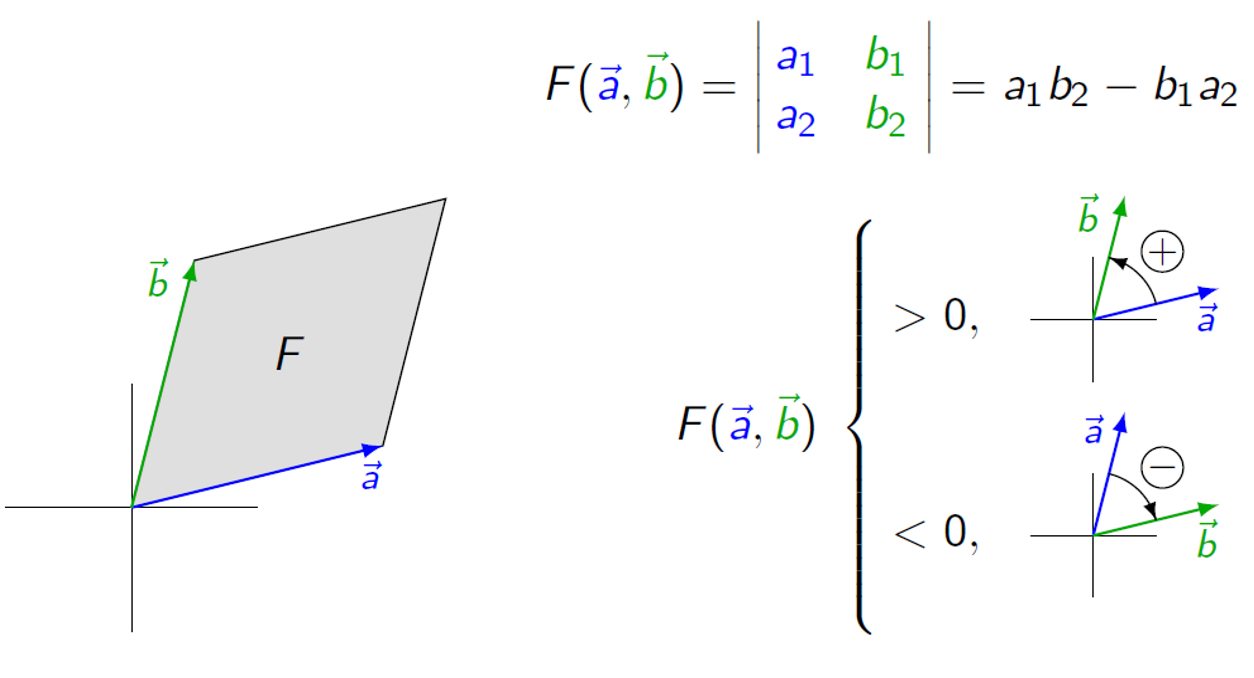
\includegraphics[width=0.7\linewidth]{Bilder/flaeche-det} \\
			
			
			\subsubsection{Volumen}				    
		    Orientiertes Volumen eines Parallelepipeds (Spat) aufgespannt durch die Vektoren $\vec{a}$, $\vec{b}$ und $\vec{c}$ \\
			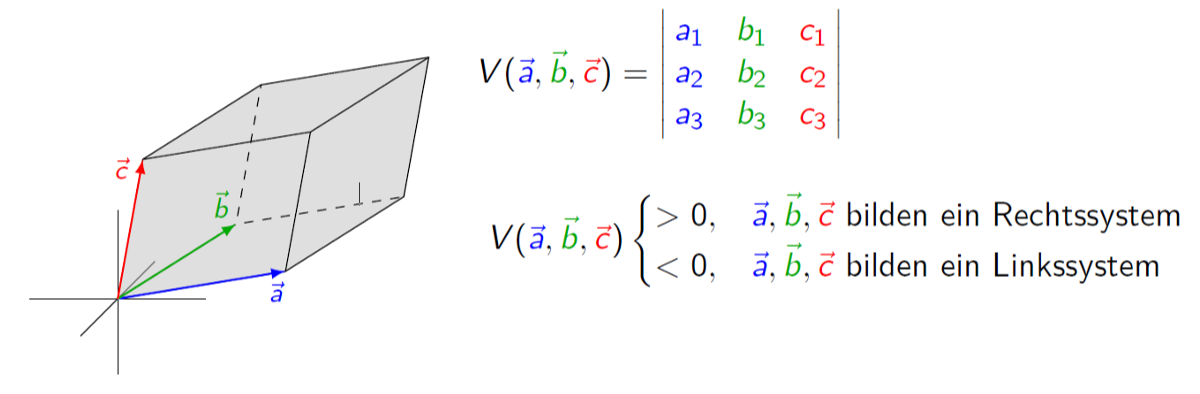
\includegraphics[width=0.9\linewidth]{Bilder/volumen-det} \\
				
				
				
			\hfill\null	
			\columnbreak	
			
			
							
								
			\subsection{Allgemeine Berechnung der Determinante}
			Die Determinante kann mithilfe des Gauss-Algorithmus berechnet werden. Die Determinante ist das \textbf{Produkt} aller Pivot-Elemente. \\
			(Rückwärts-Einsetzen beim Gauss-Verfahren nicht nötig) \\
			\\
			 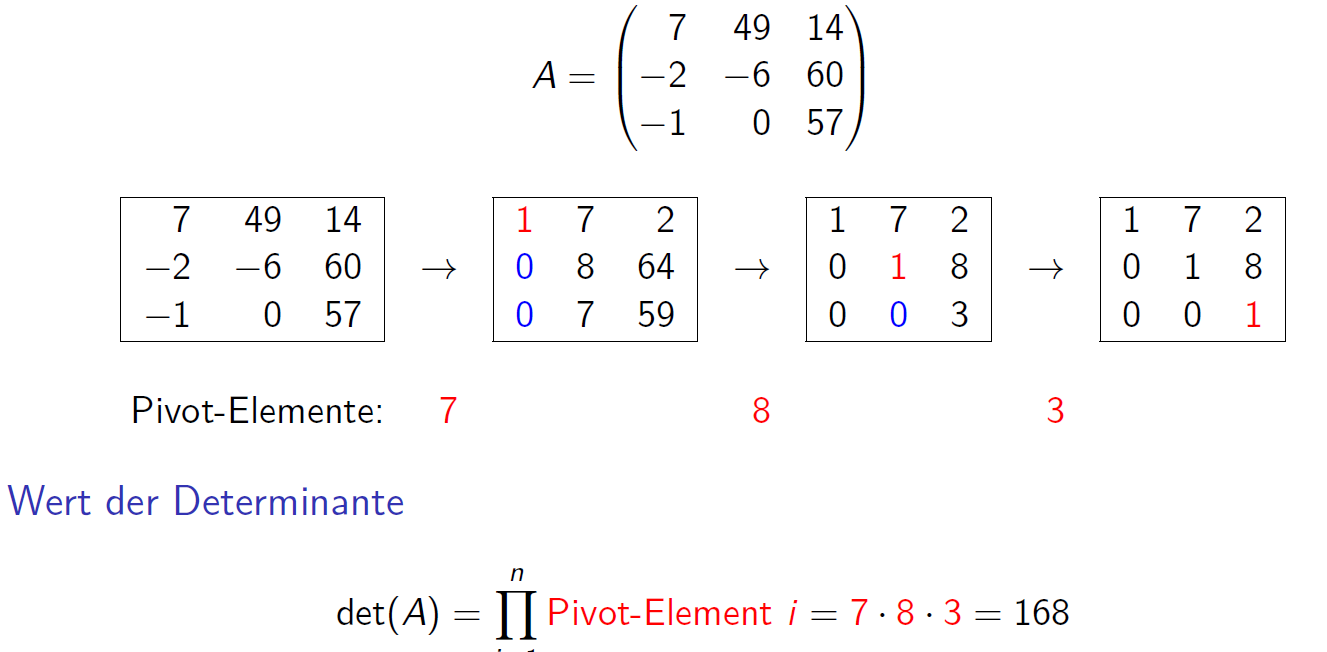
\includegraphics[width=0.8\linewidth]{Bilder/wert-determinante}
			 

		    \subsection{Sarrus}
		    \subsubsection{2 x 2 Matrix}
		    $\det(A) \quad= 	\begin{vmatrix}
		    				a & b \\
		    				c & d
		    				\end{vmatrix}$ =  $ad - bc$ \\
		    	
		    	\subsubsection{3 x 3 Matrix}
		    $\det(A) \quad= 	\begin{vmatrix}
		    					a & b &c \\
		    					d & e & f\\
		    					g & h & i
		    				\end{vmatrix}$ =  $aei + bfg + cdh - ceg - afh - bdi$ \\
		    				
		    				
		    \subsection{Rechenregeln für die Determinante}
			\begin{tabular}{ll}
			1. & Enthält A eine Nullzeile/Nullspalte, dann gilt $\det(A) = 0$ \\
		    2. & Sind zwei Zeilen/Spalten der Matrix A gleich, gilt $\det(A) = 0$ \\
		    3. &  Vertauscht man in der Matrix A zwei Zeilen/Spalten, \\
		    &  so ändert das Vorzeichen von $\det(A)$ \\
		    4. & $\det(E) = 1$ \\
		    5. & Die Determinante ist eine lineare Funktion der Zeilen/Spalten \\
		    \\
			\end{tabular}
		    
		    \begin{tabular}{ll}
		    Produktformel: &$\det(A \cdot B) = \det(A) \cdot \det(B)$ \\
		    \\
		    Determinante der Inversen: & $\det(A^{-1}) = \frac{1}{\det(A)}$ \\
		    \\
		    Transponierte Matrix: & $\det(A) = \det(A^T)$ \\
		    \end{tabular}
		    
		    
		    \subsection{Entwicklungssatz}
			
		    \begin{tabular}{ll}
			1. & Zeile oder Spalte mit meisten Nullen auswählen \\
			2. & Element herausschreiben \textbf{(Vorzeichenmatrix beachten!)} \\
			& herausgenommene Elemente, welche 0 sind fallen weg! \\
			3. & Zeile und Spalte von gewähltem Element wegdenken\\
			4. & Rest (Minor) als Determinante mit herausgenommenem \\
			& Element multiplizieren \\
			5. & Schritte 2-4 wiederholen, bis ganze Zeile/Spalte bearbeitet ist \\
			6. & Wenn noch keine 3x3 Determinanten; Schritte 1-5 wiederholen \\
			7. & Wenn 3x3 Determinanten erreicht sind, mit Sarrus-Formel \\
			& Minor-Determinanten konkret ausrechnen	\\	    		
		    \end{tabular}

			
		    \textbf{Vorzeichenmatrix} \\
		    
		    \begin{tabular}{| c | c | c | c |}
		    \hline
		    + & - & + & - \\
		    \hline
		    - & + & - & + \\
		    \hline
		    + & - & + & - \\
		    \hline
		    - & + & - & + \\
		    \hline
		    \end{tabular}
					    
		    \subsubsection{Beispiel Entwicklungssatz}
		    Berechnung der Determinante von Matrix $A$ \\
		    $A = \begin{pmatrix}
		    		4 & 0 & 7 & 0 \\
		    		5 & 8 & 5 & 1 \\
		    		4 & 7 & 4 & 1 \\
		    		8 & 8 & 10 & 1 \\
		    		\end{pmatrix}$ \\
		    		
		    	\vspace{0.3cm}
			
			$\begin{vmatrix}
		    	\color{blue}4 & \color{blue}0 & \color{blue}7 & \color{blue}0 \\
		    	5 & 8 & 5 & 1 \\
		    	4 & 7 & 4 & 1 \\
		    	8 & 8 & 10 & 1 
		    	\end{vmatrix}  =  4 	\begin{vmatrix}
		    						 8 & 5 & 1 \\ 7 & 4 & 1 \\ 8 									& 10 & 1 
								\end{vmatrix} + 7 												\begin{vmatrix}
								5 & 8 & 1 \\ 4 & 7 & 1 \\ 8 & 								8 & 1 
								\end{vmatrix}$ \quad $\rightarrow$ Sarrus \\						 		    
		    
			\subsubsection{Beispiel Inverse Matrix mittels Entwicklungssatz}
			
			$A = \begin{pmatrix}
		    		-1 & \color{blue}-3 & \color{orange}1 \\
		    		\color{green}3 & 3 & \color{red}-2  \\
		    		\color{teal}2 & \color{violet}1 & -3  \\
		    		\end{pmatrix}$  \quad  \begin{tabular}{ll}
		    		1. & det(A) berechnen \\
		    		2. & Minoren gemäss Entwicklungssatz \\
		    		& in $A^{-1}$ schreiben \\
		    		& \textbf{Farben beachten!} \\
		    		3.& Minoren mit Sarrus berechnen \\
		    		\\
					\end{tabular}						

			$A^{-1} = \frac{1}{\det(A)} \begin{pmatrix}
			\begin{vmatrix}	3 & -2 \\ 1 & -3 \end{vmatrix} & \textcolor{green}{- \begin{vmatrix}	-3 & 1 \\ 1 & -3 \end{vmatrix}} & \textcolor{teal}{\begin{vmatrix}	-3 & 1 \\ 3 & -2 \end{vmatrix}} \\
			\\
			\textcolor{blue}{- \begin{vmatrix}	3 & -2 \\ 2 & -3 \end{vmatrix}} & \begin{vmatrix}	-1 & 1 \\ 2 & -3 \end{vmatrix} & 	\textcolor{violet}{- \begin{vmatrix}	-1 & 1 \\ 3 & -2 \end{vmatrix}} \\
			\\
			\textcolor{orange}{\begin{vmatrix}	3 & 3 \\ 2 & 1 \end{vmatrix}} & \textcolor{red}{- \begin{vmatrix}	-1 & -3 \\ 2 & 1 \end{vmatrix}} & \begin{vmatrix}	-1 & -3 \\ 3 & 3 \end{vmatrix} 
									\end{pmatrix}$ \\ \\
				$\rightarrow$ Sarrus-Formel anwenden \\
										
		    
		    \subsection{Cramersche Regel}
			Mit der Cramerschen Regel können ebenfalls Gleichungssysteme von Typ $A \cdot x = b$ gelöst werden. \\
			Jede Unbekannte x wird durch Determinanten berechnet. \\
			\\
			$\rightarrow$ Es müssen n-1 Determinanten berechnet werden!	 \\
			
			\vfill\null
			\columnbreak
			
			
			
			
			\subsubsection{Beispiel Cramersche Regel}
			$A = \begin{pmatrix}
				-1 & -3 & 0 \\
				2 & 3 & -2 \\
				2 & 1 & -3
				\end{pmatrix}$ \qquad $b = \begin{pmatrix}											\color{blue}-7 \\ \color{blue}2 \\ \color{blue}-5	
											\end{pmatrix}$ \\
				\\		
				\\ $x_1 = \frac{\begin{vmatrix}
							\color{blue}-7 & -3 & 0 \\
							\color{blue}2 & 3 & -2 \\
							\color{blue}-5 & 1 & -3 \\
							\end{vmatrix}}{\det(A)} = 1$ \qquad  $x_2 = \frac{\begin{vmatrix}
							-1 & \color{blue}-7 & 0 \\
							2 & \color{blue}2 & -2 \\
							2 & \color{blue}-5 & -3 \\
							\end{vmatrix}}{\det(A)} = 2$ \\
							
							\vspace{0.2cm}
				$x_3 = \frac{\begin{vmatrix}
							-1 & -3 & \color{blue}-7 \\
							2 & 3 & \color{blue}2 \\
							2 & 1 & \color{blue}-5 \\
							\end{vmatrix}}{\det(A)} = 3$ \\			
		    
		    
			\subsection{Matritzengruppen}	
			 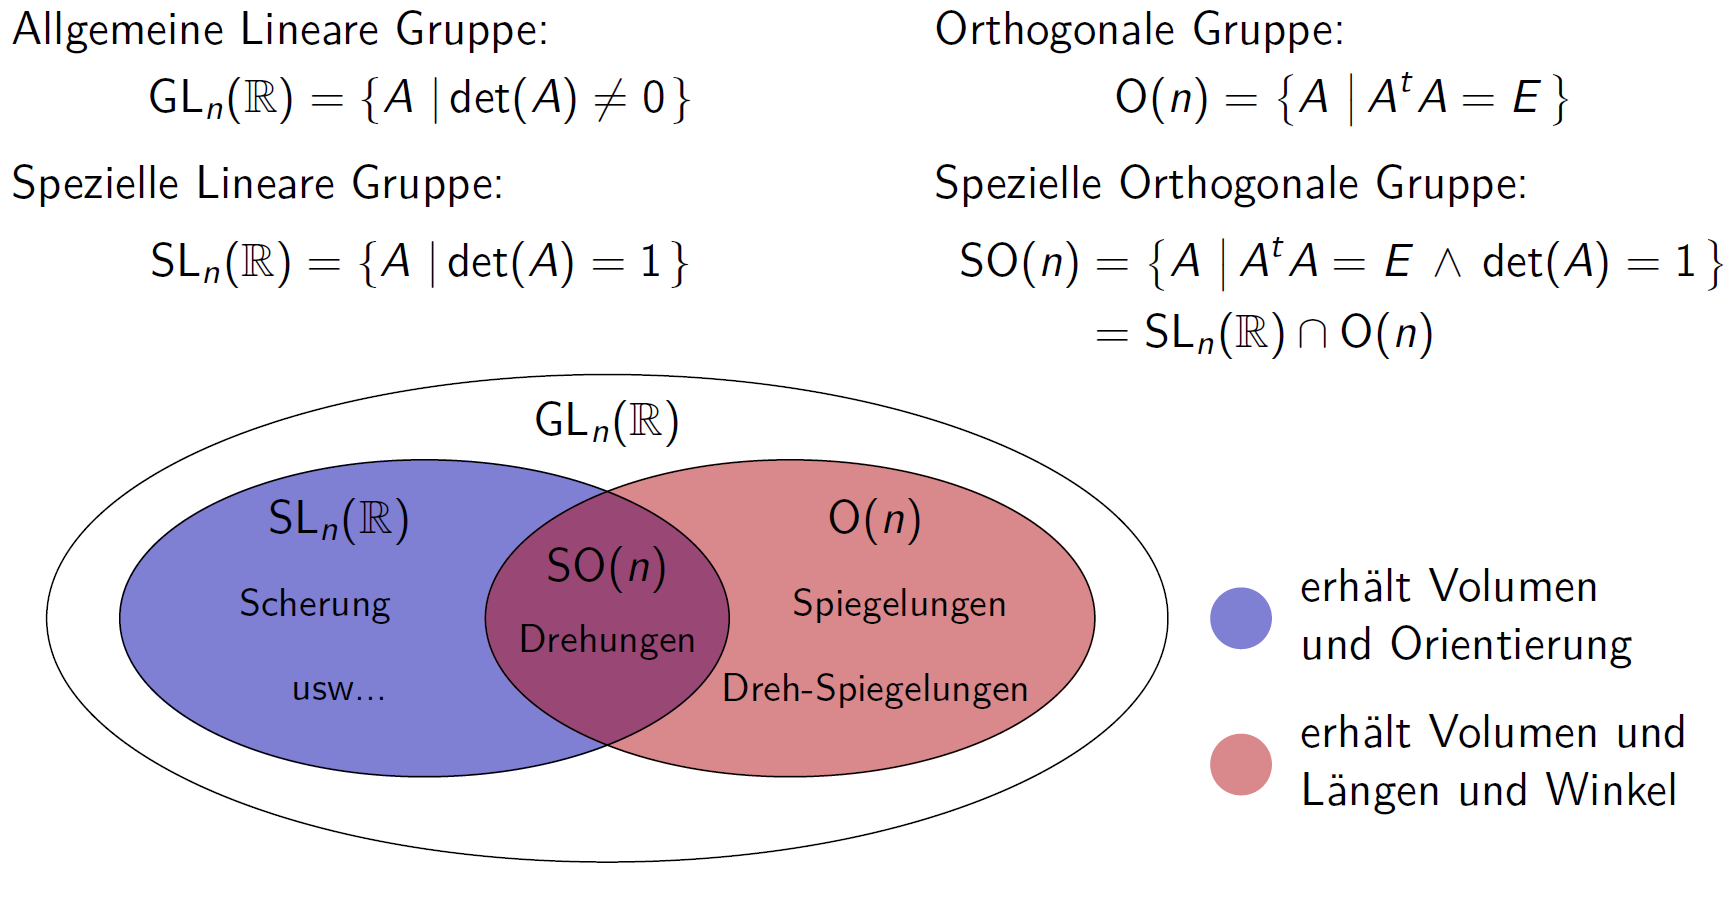
\includegraphics[width=0.8\linewidth]{Bilder/matritzengruppen} \\
		    
		 \section{Lineare Vektorräume} 
		  
		  	\subsection{Koordinatensystem}
		  	Ein Koordinatensystem ist festgelegt durch: \\
		  	\begin{tabular}{ll}
		  	$\bullet$ & Ursprung O \\
		  	$\bullet$ & Basis bestehend aus linear unabh. Basisvekoren \textcolor{blue}{$b_i$} \\
		  	\\
		  	\end{tabular}
		  	
		  	Ortsvektor: \quad Vektor $\vv{OP}$ = $\vec{p}$ = $x_1 \cdot \textcolor{blue}{\vec{b_1}} + x_2 \cdot \textcolor{blue}{\vec{b_2}}$ \\
		  	\\
		  	$x_1$ und $x_2$ sind Koordinaten des Punktes P bzw. \\
		  	Linearkombinationen der Basisvektoren \textcolor{blue}{$b_i$}
		  	
		  	
			\subsection{Vektorraum  $\langle A \rangle$}		  
			Menge aller Koordinaten (Linearkombinationen), welche durch die Vektoren $A = \vec{a_1}, ... , \vec{a_n}$ erreicht werden können. \\
			\\
			Durch bilden weiterer Linearkombinationen (Skalierungen) der \\			
			Vektoren $\vec{a_i}$ verlässt man den Vektorraum nicht.\\
			\\
			Auch Additionen / Subtaktionen von Vektoren des Vektorraums verlassen den Verktorraum nicht. \\

			\subsubsection{Dimension}
			Die Dimension $\dim \langle A \rangle$ des Vektorraums besteht aus der maximalen Anzahl linear unabhängiger Vektoren im Vektorraum. \\
			$\rightarrow$ Linear abhängige Vektoren ändern die Dimension nicht!	  	
		  	
	  	
		  	\subsection{Basis eines Vektorraums}
		  	Die Basis eines Vektorraus muss die folgenden Kriterien erfüllen: \\
		  	\begin{tabular}{ll}
		  	1. & Lineare Unabhängigkeit der Basisvektoren \textcolor{blue}{$b_i$}, damit \\  
		  	& Koordinaten \textcolor{orange}{$x_i$} eindeutig sind \\
		  	2. & Basisvektoren \textcolor{blue}{$\vec{b_i}$} müssen den ganzen Vektorraum aufspannen \\
		  	\\
		  	\end{tabular}
		  		
		  	$\vec{p} = \textcolor{orange}{x_1} \cdot \textcolor{blue}{\vec{b_1}} + \textcolor{orange}{x_2} \cdot \textcolor{blue}{\vec{b_2}} + \textcolor{orange}{x_3} \cdot \textcolor{blue}{\vec{b_3}}$  = \textcolor{blue}{B} \textcolor{orange}x = $\begin{pmatrix}
1 & 0 & 0 \\ 0 & 1 & 0 \\ 0 & 0 & 1 	\end{pmatrix} \begin{pmatrix}
x_1 \\ x_2 \\ x_3
\end{pmatrix}$ \\

\vspace{0.2cm}

$\vec{b_1}$, $\vec{b_2}$ und $\vec{b_3}$ sind im Beispiel die Standardbasisvektoren. Es können aber auch irgendwelche Vektoren einer anderen Basis sein.


		  	
			\subsection{Basistransformation}		  	
			Basismatrix B = $\lbrace \vec{b_1}, \vec{b_2}, \vec{b_3} \rbrace$ \qquad Basismatrix B' = $\lbrace \vec{b_1'}, \vec{b_2'}, \vec{b_3'} \rbrace$		\\
	
			Vektor $\vec{v}$ = $\xi B$ = $\xi' B'$ in Koordinatensystem $\xi$ und $\xi'$
 
			\subsubsection{Basistransformation allgemeiner Fall}
			Transformationsmatrix T mittels Gauss-Algorithmus finden: \\
			\begin{minipage}{0.6\linewidth}
			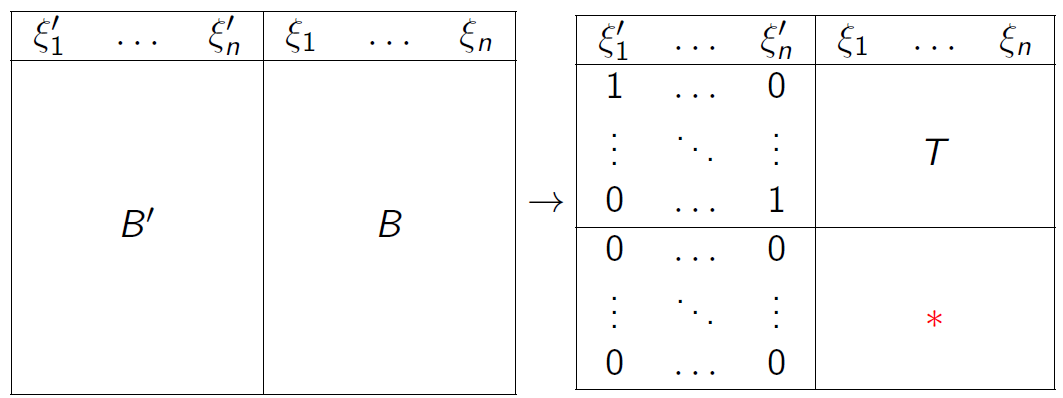
\includegraphics[width=\linewidth]{Bilder/transformationsmatrix} \\
			\end{minipage}
			\hfill
			\begin{minipage}{0.38\linewidth}
			$$ \text{Umrechnung:} \quad \xi' = T \xi$$
			\\
			\end{minipage}

			Die roten Sterne müssen Nullen sein, damit es eine Lösung gibt! 
			

			\subsubsection{Spezialfall Basistransformation (quadratische Matritzen)}		  
			\begin{tabular}{ll}
			Transfotmationsmatrix $T$ &  $T = (B')^{-1} B $	\\
			Koordinaten $\xi'$ in neuem Koordinatensystem: & $\xi = T \xi$ \\
			\end{tabular}				
				  	
		  	
		  	\subsection{Lineare Abbildungen (Bilder des Vektoraums)}
		  	\begin{tabular}{ll}
		  	Eine lineare Abbildung: & $\bullet$ bildet Geraden auf Geraden ab \\
		  	& $\bullet$ erhält Parallelität \\
		  	& $\bullet$ fixiert den Ursprung
		  	\end{tabular}
			
			Lineare Abbildungen werden mit der Abbildungsmatrix A \\
			beschrieben. \\		
			\textbf{Die Spalten von A sind Bilder der Basisvektoren} \\
			\\
			Eine Abbildung A kann durch ihre Inverse $A^{-1}$ rückgängig gemacht werden.
			
			
			
			
			\subsubsection{Beispiel Abbildungsmatrix A einer Scherung}
			Die Standardbasisvektoren $\vec{e_1}$ und $\vec{e_2}$ werden durch die Abbildungsmatrix $A$ auf die Vektoren $\vec{e_1'}$ und $\vec{e_2'}$ abgbildet. \\
			Die Spalten der Abbildungsmatrix A enthalten die Bilder $\vec{e_1'}$ und $\vec{e_2'}$ der Standardbasisvektoren 	$\vec{e_1}$ und $\vec{e_2}$ \\

			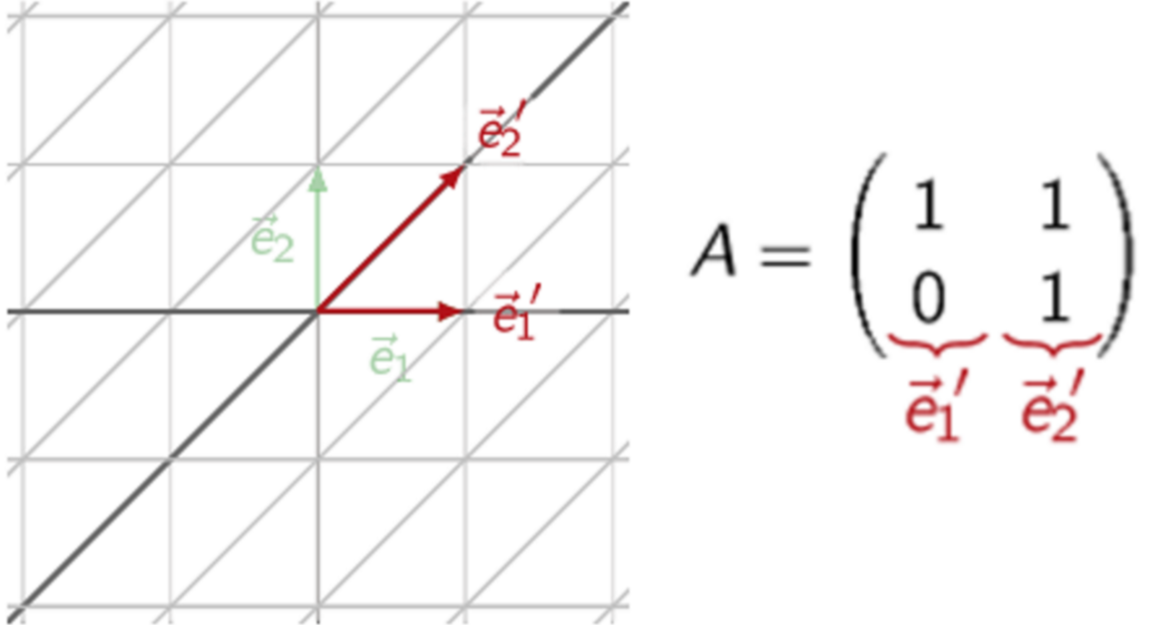
\includegraphics[width=0.5\linewidth]{Bilder/scherung}
			\subsubsection{Anwendung einer Abbildung auf einen Vektor}
			Der Vektor $\vec{v}$ wird mit der Abbildungsmatrix auf den Vektor $\vec{v'}$\\
			abgebildet: $A \cdot \vec{v} = \vec{v'}$ \\		
			\\		
			Die Abbildung kann mittels $A^{-1} \cdot \vec{v'} = \vec{v}$ rückgängig gemacht werden. \\
			\textbf{Das geht nur, wenn A eine quadratische Matrix ist!}

		  	\subsubsection{Zusammensetzung linearer Abbildungen}
		  	Wenn mehrere lineare Abbildungen "wirken", so werden die \\
		  	Abbildngsmatritzen multipliziert. \\
		  	\\
		  	\textbf{Die als erstes wirkende Abbildung steht dabei ganz rechts in der Multiplikation!}\\
		  	\\
		  	Abbildungsmatrix C = AB $\rightarrow$ Erst wirkt Abbildungsmatrix B,\\ 
		  	danach A
		  	
		  	
		  	\subsection{Kern einer Matrix}		
			Alle Abbildungen eines Vektors $\vec{v}$ , welche durch die \\
			Abbildungsmatrix $A$ auf den Nullvektor von $\vec{v'}$ abgebildet werden \\
			$A \cdot \vec{v} = 0 $ $\rightarrow$ Nullraum, Kern von $A$, ker($A$) 
			
			
			\subsection{Bild einer Matrix}		
			Menge der Vektoren, welche man aus den Spalten einer Matrix \\
			erzeugen kann.\\
			\\
			Das Bild besteht aus allen Vektoren, welche unter der Abbildung, die $B$ vermittelt, wentstehen können.
			
			
			
			
			\subsection{Kern, Bild und Gauss-Algorithmus}	
			Die Lösungsmenge entspricht dem Kern von $A$ bzw. dem Bild von $B$ \\	
			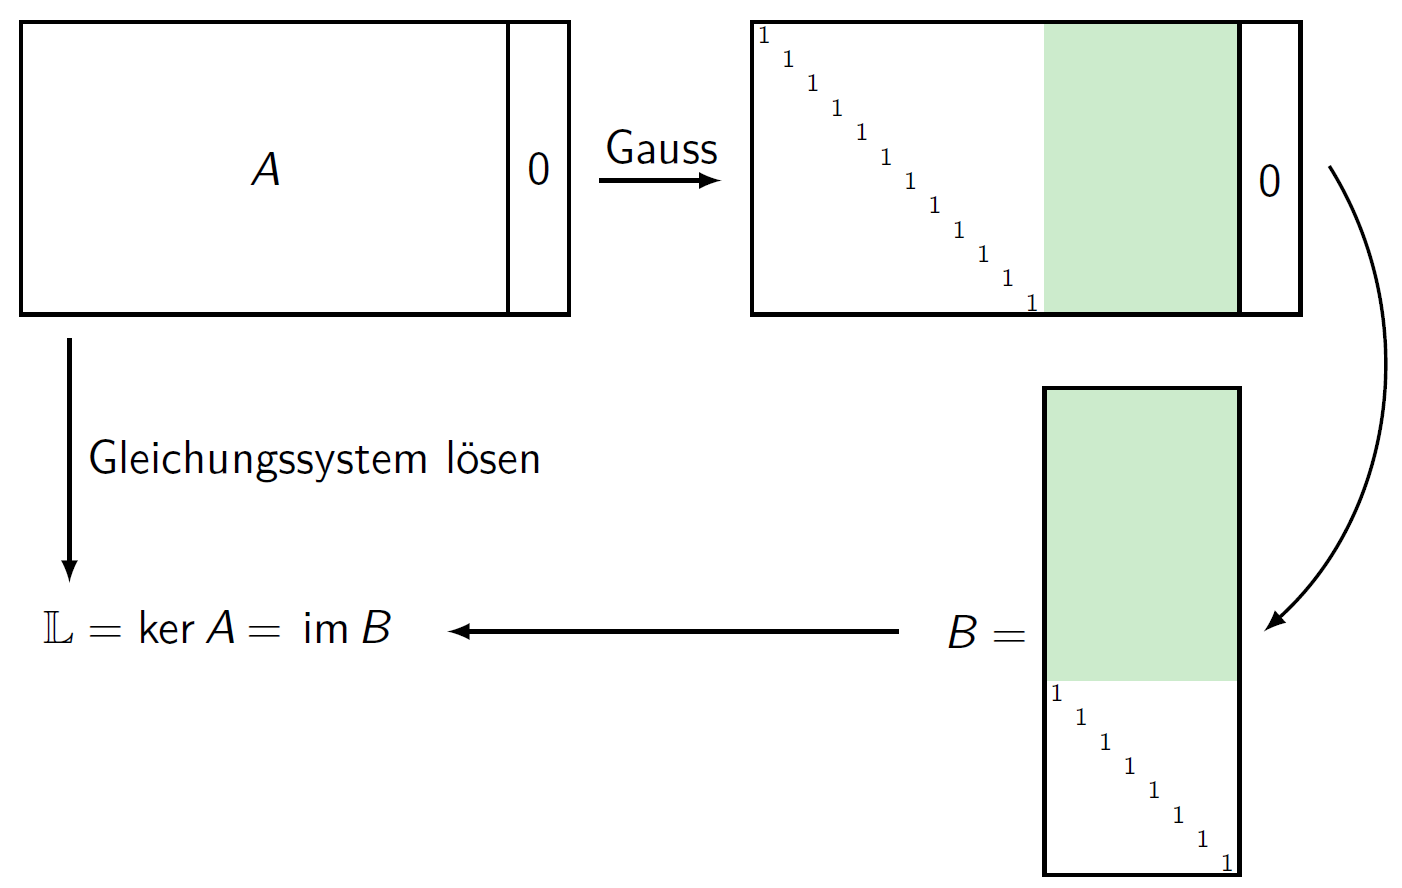
\includegraphics[width=0.55\linewidth]{Bilder/kern-bild-gauss} 	
			
			
			\subsection{Basiswechsel für lineare Abbildungen}
			Die lineare Abbildung, die in der Basis $B$ durch die Matrix $A$ beschrieben wird, wird in der Basis $C$ durch die Matrix $A'$ beschrieben.\\
			
			\begin{minipage}{0.6\linewidth}
			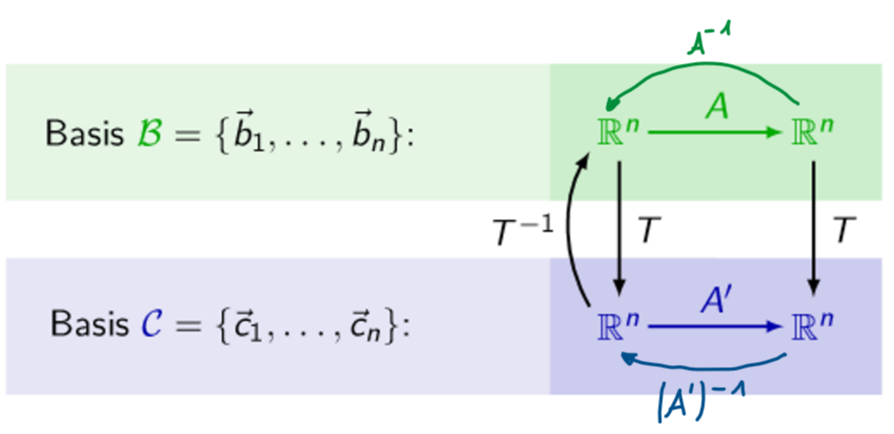
\includegraphics[width=0.9\linewidth]{Bilder/basiswechsel_abbildungen}
			\end{minipage}						
			\hfill
			\begin{minipage}{0.35\linewidth}
			$\textcolor{blue}{A'} = T \textcolor{green}A \,T^{-1}$ \\
			$\det(A') = \det(A)$ \\
			Spur($A'$) = Spur($A$)	
			\end{minipage}
	
		  	
		  	\subsection{Elementare Abbildungsmatritzten}
		  	\subsubsection{Drehmatrix D finden}
			Die Drehung wird beschrieben durch $D \cdot A = A'$		  	 \\
			Die Spalten der Matrix $A$ sind die Punkte vor der Drehung, $A'$ enthält die Punkte nach der Drehung (Bilder)\\
			$D = A' \cdot A^{-1}$ \\
			\textbf{Die Matritzten müssen quadratisch sein! Falls nötig Matritzen mit einem Punkt erweitern, damit sie quadratisch werden}
		  	
		  	
		  	\subsubsection{Spiegelungen (orthogonale Matrix)}
		  	$\det(A) = -1$ \\
		  	\\
		  	\textbf{2 Dimensionen} \\
		  	\\
		  	\begin{tabular}{lll}
		  	x-Achse & y-Achse & an 45° Geraden \\
		  	\\
		  	$\begin{pmatrix} 1 & 0 \\ 0 & -1 \end{pmatrix}$ & $\begin{pmatrix} -1 & 0 \\ 0 & 1 \end{pmatrix}$ & $\begin{pmatrix} 0 & 1 \\ 1 & 0 \end{pmatrix}$ \\
		  	\\
		  	\end{tabular}
		  	
			\textbf{3 Dimensionen} \\
		  	\\
		  	\begin{tabular}{lll}
		  	xy-Ebene & xz-Ebene & an yz-Ebene\\
		  	\\
		  	$\begin{pmatrix} 1 & 0 & 0 \\ 0 & 1 & 0 \\ 0 & 0 & -1 \end{pmatrix}$ & $\begin{pmatrix} 1 & 0 & 0 \\ 0 & -1 & 0 \\ 0 & 0 & 1 \end{pmatrix}$ & $\begin{pmatrix} -1 & 0 & 0 \\ 0 & 1 & 0 \\ 0 & 0 & 1 \end{pmatrix}$ \\
		  	\end{tabular}		  	
		  	
			\subsubsection{Projektionen}		
			Projektionen auf etwas (z.B. die Koordinatenachsen) liefern die "Länge des Schattens" des Vektors auf diese Achse. \qquad $P^2 = P$ \\
			\\
			\begin{tabular}{ll}
		  	x-Achse & y-Achse \\
		  	\\
		  	$\begin{pmatrix} 1 & 0  \\ 0 & 0  \end{pmatrix}$ & $\begin{pmatrix} 0 & 0  \\ 1 & 0  \end{pmatrix}$  \\
		  	\\
		  	\end{tabular}				
			
			\begin{tabular}{lll}
		  	xy-Ebene & xz-Ebene & an yz-Ebene\\
		  	\\
		  	$\begin{pmatrix} 1 & 0 & 0 \\ 0 & 1 & 0 \\ 0 & 0 & 0 \end{pmatrix}$ & $\begin{pmatrix} 1 & 0 & 0 \\ 0 & 0 & 0 \\ 0 & 0 & 1 \end{pmatrix}$ & $\begin{pmatrix} 0 & 0 & 0 \\ 0 & 1 & 0 \\ 0 & 0 & 1 \end{pmatrix}$ \\
		  	\end{tabular}		  	
		  	
		  	\subsubsection{Drehungen D (orthogonale Matrix)}
		  	Die Spalten von $D_{\alpha}$ sind Bilder der Basisvektoren \\
		  	Determinante: \quad $\det(D) = 1$\\	
		  	\\
		  	Die Drehung findet gegen den Uhrzeigersinn statt \\
		  	Für Drehung in Uhrzeigersinn: $D_{-\alpha} = D_{\alpha}^{-1}$ verwenden \\
		  	$D_{\alpha} D_{\beta} = D_{\alpha + \beta}$ \\
		  	
			\columnbreak
					  	
		  	\textbf{2 Dimensionen} \\
		  	\\
		  	$D_{\alpha} = \begin{pmatrix} \cos(\alpha) & -\sin(\alpha)  \\ \sin(\alpha) & \cos(\alpha)  \end{pmatrix}$ \\
		  	
			\textbf{3 Dimensionen} \\
			\\
			\begin{tabular}{ll}
			Drehung um x-Achse & Drehung um y-Achse \\
			\\
			$D_{x} = \begin{pmatrix} 1 & 0 & 0 \\\
			0 & \cos(\alpha) & -\sin(\alpha)  \\ 0 & \sin(\alpha) & \cos(\alpha)  \end{pmatrix}$ & $D_{y} = \begin{pmatrix} \cos(\alpha) & 0 & \sin(\alpha) \\
			0 & 1 & 0 \\ -\sin(\alpha) & 0 & \cos(\alpha)  \end{pmatrix}$\\
			\\
			Drehung um z-Achse & \\
			\\
			$D_{z} = \begin{pmatrix} \cos(\alpha) & -\sin(\alpha) & 0 \\ \sin(\alpha) & \cos(\alpha) & 0 \\ 0 & 0 & 1 \end{pmatrix}$
			\end{tabular}
		  	
		  	
			\subsection{Drehwinkel von Drehmatritzen D}		  	
			Der Drehwinkel einer Drehmatrix $D$ wird mithilfe der Spur der \\
			Drehmatrix berechnet (siehe nächster Abschnitt) \\ 	
			\\	  			
			\begin{tabular}{lll}
			\textbf{2 Dimensionen} & & \textbf{3 Dimensionen} \\
			\\
			$\cos(\alpha) = \frac{\mathrm{Spur}(D)}{2}$ & & $\cos(\alpha) = \frac{\mathrm{Spur}(D) -1}{2}$
			\end{tabular}		  	
		  	
		  	
			\subsection{Spur}		  	
			Die Spur einer Matrix ist die Summe der Elemente auf der Diagonalen \\
			
			$A =  \begin{pmatrix}	\textcolor{blue}{1} & 7 & 9 \\ 2 & \textcolor{blue}{9} & 6 \\ 8 & 3 & \textcolor{blue}{5}	\end{pmatrix}$	   \qquad 	$\mathrm{Spur}(A) = \textcolor{blue}{1} + \textcolor{blue}{9} + \textcolor{blue}{5} = 15$ 
		  	
		  	\subsubsection{Rechenregeln Spur}
		  	\begin{tabular}{ll}
		  	Vertauschung & Spur($BA$) = Spur($AB$) \\
		  	Zykl. Vertauschung: & Spur($ABC$) = Spur($CAB$) = Spur($BCA$)\\
		  	Anwendung: & Spur($TAT^{-1}$) = Spur($T^{-1}TA$)= Spur($A$)\\
		  	\end{tabular}
		  	
		\section{Vektorgeometrie}
		  Generell gilt auf dieser Zusammenfassung: \\
			
			\begin{tabular}{ll}
			$\vec{p}$ & Ortsvektor (Vektor vom Ursprung zu Punkt auf Geraden)\\
			$\vec{r}$ & Richtungsvektor \\
			$\vec{x}$ & Platzhalter für Punkt (auf Ebene / Geraden) $x_1, x_2, x_3$ \\
			$s, t, u, v$ & Variablen $\in \mathbb{R}$ \\
			\end{tabular}						
			
			
			\subsection{Normalenvektor}		    
		   	Der Normalenvektor einer Geraden / Ebene steht senkrecht auf der Geraden / Ebene.	\\
		   	Der Normalenvektor kann mit dem Vektorprodukt oder dem  \\
		   	Skalarprodukt berechnet werden\\
		   	\\
		   	\begin{tabular}{ll}
		   	Vektorprodukt: & $\vec{n} =  \vec{r_1} \times \vec{r_2}$ \\
		   	Skalarpodukt: & $\vec{n} \bullet \vec{r_1} = 0$ und $\vec{n} \bullet \vec{r_2} = 0$  \\
		   	& Skalarprodukte als Gleichung aufschreiben \\
		   	& $\rightarrow$ Gauss-Tableau  $\rightarrow$ Normalenvektor \\
		   	& (es gibt eine frei wählbare Variable) \\
			\end{tabular}		   			
			
			
		    \subsection{Darstellungsformen von Ebenen / Geraden}	
		    
			\subsubsection{Koordinatenform}	% unsicher ob korrekt
			\begin{tabular}{lll}
			Ebene: & $\textcolor{red}{n_x} \, x_1 + \textcolor{red}{n_y} \, x_2 + \textcolor{red}{n_z} \, x_3 = b$ & $\textcolor{red}{5} \, x_1 + \textcolor{red}{10} \, x_2 \textcolor{red}{- 2} \, x_3 = 6 $ \\
			\\
			Gerade: &  $\textcolor{red}{n_x} \, x_1 + \textcolor{red}{n_y} \, x_2  = b$ & $\textcolor{red}{5} \, x_1 + \textcolor{red}{10} \, x_2 = 6 $ \\
			\\
			\end{tabular}						    

		    Die roten Koeffizienten entsprechen den Koordinaten des \\
		    Normalenvektors. \\
		    $b$ entspricht dem Abstand der Ebene zum Nullpunkt des \\
		    Koordinatensystems.
	    
	    
	
		    
		    
			\subsubsection{Parameterform}
			Hinweis: in 2 Dimensionen ohne z-Koordinate, ansonsten analog \\			
			
			Gerade g: \quad $\vec{p} + s \cdot \vec{r} = \begin{pmatrix} p_x \\ p_y \\ p_z \end{pmatrix}	+ t \cdot \begin{pmatrix} r_x \\ r_y \\ r_z \end{pmatrix}$ \\
			\\

			Ebene E: \quad $\vec{p} + s \cdot \vec{r_1} + t \cdot \vec{r_2} = \begin{pmatrix} p_x \\ p_y \\ p_z \end{pmatrix}	+ s \cdot \begin{pmatrix} r1_x \\ r1_y \\ r1_z \end{pmatrix} + t \cdot \begin{pmatrix} r2_x \\ r2_y \\ r3_z \end{pmatrix}$ 
			
			
			\subsubsection{Normalenform}		   
			\begin{minipage}{0.48\linewidth}
			Gerade g: \quad $\vec{n} \bullet (\vec{x} - \vec{p}) = 0$ \\
			\end{minipage}	
			\hfill	
			\begin{minipage}{0.48\linewidth}
			Ebene E: \quad $\vec{n} \bullet (\vec{x} - \vec{p}) = 0$ \\
			\end{minipage}	 
		    
			Wenn $\neq 0$ liegt der Punkt x nicht auf der Geraden / Ebene 
			
			
		    \subsubsection{Umrechnungen der verschiedenen Formen}
		    \textbf{Koordinatenform in Parameterform}\\
		    \\
		    \begin{tabular}{ll}
		    1. & Normalenvektor aus Koordinatengleichung ablesen \\
		    & Koordinatengleichung einsetzen \\
		    2. & Richtungsvektoren aus den 3 Punkten bilden \\
		    3. & Parameterform aufstellen \\
		    \\
		    \end{tabular}
		    

		    	\textbf{Koordinatenform in Normalenform} \\
		    	\\
		    	\begin{tabular}{ll}
		    1. & 3 Punkte auf Ebene bestimmen  Spurpunkte in \\
		    & Koordinatengleichung einsetzen \\
		    2. & Punkt auf Ebene finden: Spurpunkt einsetzen \\
		    3. & Aus gefundenem Normalen- und Richtungsvektor \\
		    & Normalenform aufstellen \\
		    \\
		    \end{tabular}
		    
		    
			\textbf{Parameterform in Normalenform}\\
		    	\\
		    	\begin{tabular}{ll}
		    1. & aus Richtungsvektoren den Normalenvektor bilden \\
		    2. & Aus gefundenem Normalenvektor und bekanntem Stützvektor \\
		    &  die Normalenform aufstellen \\	   
		    \\
		    \end{tabular}		    
		    
		    
		    	\textbf{Parameterform in Koordinatenform}\\
			\\
		    	\begin{tabular}{ll}
		    1. &  Paramaterform Zeile für Zeile als einzelne Gleichungen \\
		    & aufschreiben \\
		    2. &  Variablen s und t schrittweise aus GlSys eliminieren  \\
		    & Vielfache einer Gleichung mit Vielfache von anderer Gleichung \\
		    & addieren/subtrahieren und somit neue Gleichungen finden \\
		    3. &  Wenn s und t eliminiert sind und die Schlussgleichung \\
		    & gefunden ist, entspricht dies der Koordinatengleichung  \\
		    \\
		    \end{tabular}		    	 
		    
		    	\textbf{Normalenform in Parameterform} \\
		    	\\
		    	\begin{tabular}{ll}
		    1. & Richtungsvektoren aus Normalenvektor finden:\\
		    & Eine Komponente des Normalenvektors 0 setzen \\
		    & $\rightarrow$ 0 in erstem Richtungsvektor \\
		    & verbleibenden Komponenten vertauscht in Richtungsvektor \\
		    & einsetzen und ein Vorzeichen tauschen \\
		    2. & Schritt 1 für zweiten Richtungsvektor wiederholen  \\
		    & Wichtig: Andere Komponente von Normalen 0 setzen! \\
		    3. & Aus Richtungsvektoren und bekannten Stützvektor \\
		    &  Parameterform aufstellen  \\	   
		    \end{tabular}	    
		    		    
		    	\vfill\null
		    	\columnbreak	    
		    		    
		    		    
		    		    
		    \subsection{Hesse'sche Normalform als Darstellungsform}
		    \textbf{In der Hesse'schen Normalform ist der Abstand d vom \\
		    Nullpunkt zur Ebene immer d = 1} 
		    
		    \subsubsection{Beispiel Umwandlung in Hessesche Normalform}
		    \begin{tabular}{ll}
		    Ebene E: & $3 x_1 + 8 x_2 - 5 x_3 = 3$ \\
		    \\
		    Hesse'sche Normalform: & $x_1 + \frac{8}{3} x_2 - \frac{5}{3} x_3 = 1$
		    \end{tabular}
		    
			
			\subsection{Orthonormalbasis}
			In einer Orthonormalbasis stehen die Basisvektoren $b_i$ senkrecht \\
			aufeinander und haben die Länge 1 \\
			\\
			Ausgedrückt mit dem Skalarprodukt bedeutet dies: \\
			\begin{tabular}{ll}
			Senkrecht aufeinander: & $\vec{b_1} \bullet \vec{b_2} = 0$ \\
			Länge 1: & $\vec{b_1} \bullet \vec{b_1} = 1$
			\end{tabular}
		  
		   
			\subsection{Skalarprodukt}
			
			\begin{minipage}{0.4\linewidth}
			\textbf{2 Dimensionen} \\
			\\
			$\vec{a} \bullet \vec{b} = \vert \vec{a} \vert \cdot \vert \vec{b} \vert \cdot \cos(\alpha)$ \\
			\\
			\\
			\\
			\\
			\end{minipage}
			\hfill
			\begin{minipage}{0.58\linewidth}
			\textbf{3 Dimensionen} \\
			\\
			$\vec{a} \bullet \vec{b} = \begin{pmatrix} a_x \\ a_y \\ a_z \end{pmatrix} \bullet \begin{pmatrix} b_x \\ b_y \\ b_z \end{pmatrix}$ \\
			\\
			wenn Basis = Orthonormalbasis!\\
			\end{minipage}
			
			

			\subsubsection{Eigenschaften des Skalarprodukts}
			
			\begin{tabular}{ll}
			Linearität & linear in $\vec{a}$ und $\vec{b}$ (bilinear) \\
			& $\rightarrow$ man kann ausmultiplizieren\\
			
			Orthagonalität: &  $\vec{a} \bullet \vec{b} = 0$ \\
			
			Länge im Quadrat: & $\vec{a} \bullet \vec{b} = \vert \vec{u} \vert ^2$ 	\\
						
			Länge: &$\sqrt{\vec{a} \bullet \vec{a}}$ \\
			
			Als Matrixprodukt: & $\vec{a}^t \vec{b} = \vec{b}^t \vec{a} = \vec{a} \bullet \vec{b}$ \\
			\\
			\end{tabular}
			
			\textbf{Winkel zwischen zwei Vektoren} \\
			\\
			$\cos(\alpha) = \frac{\vec{a} \bullet \vec{b}}{ \vert \vec{a} \vert \cdot \vert \vec{b} \vert}$ \\
			
			
			 
		    \subsection{Länge (Betrag) eines Vektors}
		    $\vert \vec{a} \vert = \sqrt{\vec{a} \bullet \vec{a}} = \sqrt{a_x^2 + a_y^2 + a_z^2}$
		    
		    \vfill\null
		    \columnbreak
		    
		    
			
			\subsection{Orthagonale Projektion mittels Skalarprodukt}
			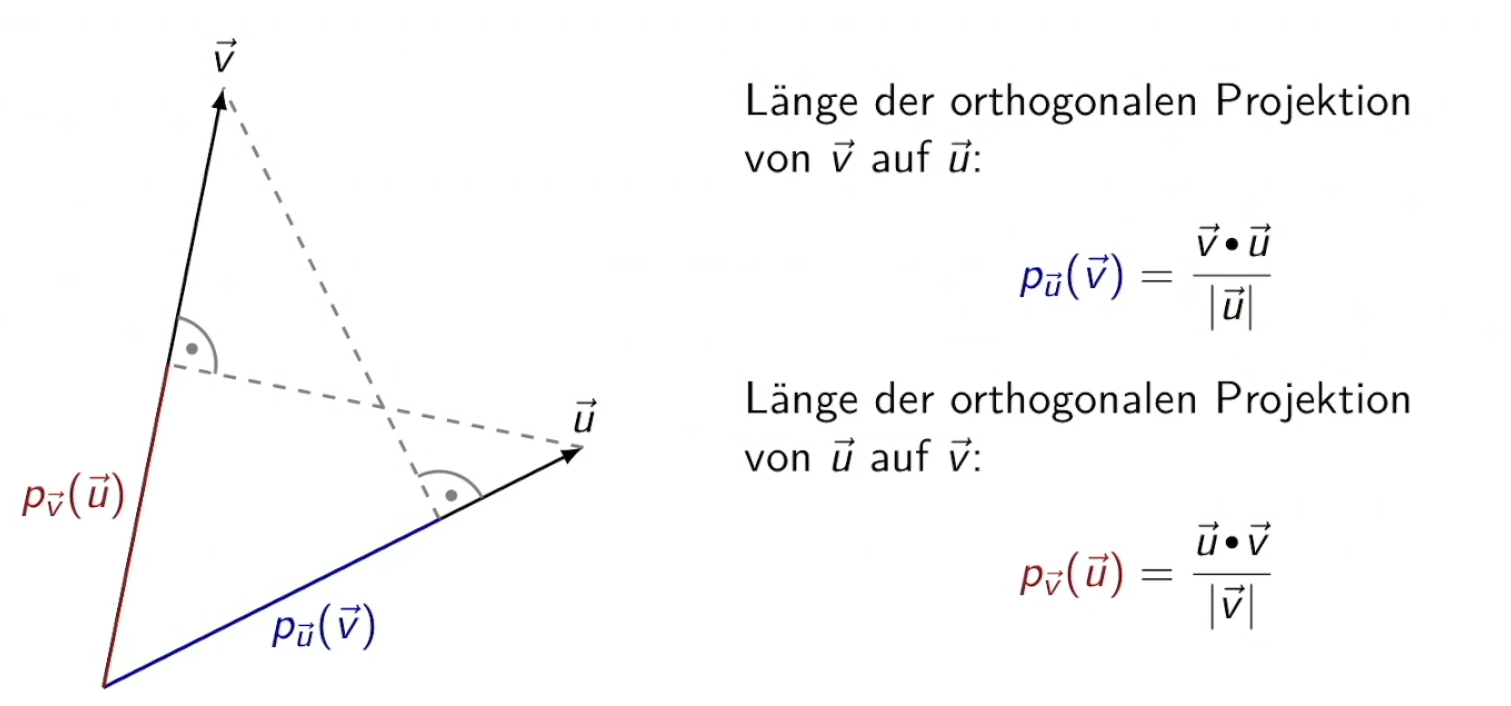
\includegraphics[width=0.65\linewidth]{Bilder/orthagonale-projektion}
			
			
			\subsection{Prallel- und Orthagonalkomponente}
			Ein Vektor kann in zwei orthagonale Komponenten aufgeteilt werden \\					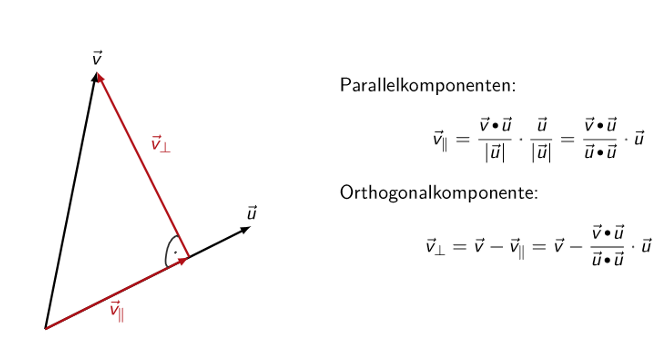
\includegraphics[width=0.65\linewidth]{Bilder/parallel-orthagonal}
			
			
			\subsection{Spiegelung}
			Der gespiegelte Vektor entspricht $\vec{v'} = \vec{v} - 2 \vec{v_{\parallel}} = \vec{v} - 2 \vec{n} \frac{\vec{n} \bullet \vec{v}}{\vert \vec{n} \vert ^2} $ \\
			\begin{minipage}[b]{.5\linewidth} 
  			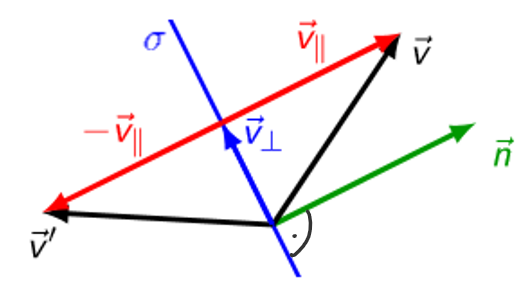
\includegraphics[width=\linewidth]{Bilder/spiegelung}
			\end{minipage}
			\hfill
			\begin{minipage}[b]{.45\linewidth} 
			Beschreibung der \\
			Spiegelnugsmatrix S: \\
			\\
			$S = E - 2 \frac{1}{\vert \vec{n} \vert ^2} \vec{n} \bullet \vec{n}^t$  	\\
			\\
			Wenn $\vec{n}$  Länge 1 hat: \\
			$S = E - 2 \vec{n}^0 \bullet \vec{n}^{0 t}$  	
			\end{minipage}						
			
			\subsection{Orthagonale Matrix / Orthagonalität}
			\textbf{Orthagonal heisst: $A^t A = E$}\\		
			Eine orthagonale Matrix ändert das Skalarprodukt nicht. \\
			\\
			Eigenschaften orthagonale Matritzten: \\
			\begin{tabular}{lll}
			$A^t A = E$ & $A^{-1} = A^t$ & $A^t$ auch orthagonal
			\end{tabular}
				
			
			\subsection{Hessesche Normalform}
			\textbf{Berechnung Abstand d von Punkt $\vec{x}$ zu Ebene}  \\
			Anwendung in Koordinatenform und Normalform möglich \\
			$\vec{q}$ entspricht dem Stützvektor der Ebene! 
			
			\subsubsection{Länge des Normalenvektors nicht 1}
			
			\begin{tabular}{lll}
			\textbf{Koordinatenform} & & \textbf{Parameterform} \\
			\\
			
			$d = \frac{n_x}{\vert \vec{n} \vert} x_1 + \frac{n_y}{\vert \vec{n} \vert} x_2 + \frac{n_z}{\vert \vec{n} \vert} x_3 - \frac{\vec{n} \bullet \vec{q}}{\vert \vec{n} \vert}$ & & $d = \frac{\vec{n} \bullet (\vec{x} - \vec{q})}{\vert \vec{n} \vert}$ \\
			\end{tabular}
			
			\vfill\null
			\columnbreak
			
			
			\subsubsection{Länge des Normalenvektors ist 1}
			
			\begin{tabular}{lll}
			\textbf{Koordinatenform} & & \textbf{Parameterform} \\
			\\
			
			$d = n_x x_1 + n_y x_2 + n_z x_3 - \vec{n} \bullet \vec{q}$ & & $d = \vec{n} \bullet (\vec{x} - \vec{q}) $
			\end{tabular}
				    
		    
		    
		    
			\subsection{Vektorprodukt (Kreuzprodukt)}		    
		    \textbf{Nur definiert in 3 Dimensionen!} \\
		    \\
		    \begin{minipage}{0.45\linewidth}
		    $\vec{a} \times \vec{b} = \begin{pmatrix} a_2 b_3 - a_3 b_2 \\ -(a_1 b_3 - a_3 b_1) \\ a_1 b_2 - a_2 b_2 \end{pmatrix}$ \\
		    \end{minipage}
		    \hfill
		    \begin{minipage}{0.5\linewidth}
		    $\vec{a} \times \vec{b} = -\vec{b} \times \vec{a}$ \\
		    $\vec{a} \times \vec{a} = 0$ \\
		    $\vec{a} \times (\vec{b} \times \vec{c}) = (\vec{a} \bullet \vec{c}) \vec{b} - (\vec{a} \bullet \vec{b}) \vec{b}$ \\
		    $(\vec{a} \times \vec{b}) \times \vec{c} = (\vec{a} \bullet \vec{c}) \vec{b} - (\vec{a} \bullet \vec{b}) \vec{b}$
		    \end{minipage}
		    
		    
		    \subsubsection{Eigenschaften des Vektorprodukts}
		    
		    \begin{tabular}{ll}
		    $\bullet$ & $\vec{a} \times \vec{b}$ ist senkrecht auf $\vec{a}$ und $\vec{b}$\\
		    & $( \vec{a} \times \vec{b}) \bullet \vec{a} = \det(\vec{a}, \vec{b}, \vec{a}) = 0$\\
		    & $( \vec{a} \times \vec{b}) \bullet \vec{b} = \det(\vec{a}, \vec{b}, \vec{b}) = 0$\\
		    $\bullet$ & $\vert \vec{a} \times \vec{b} \vert$ ist Fläche eines Parallelogramm \\ 
		    $\bullet$ & $\vec{a}, \, \vec{b}, \, \vec{a} \times \vec{b}$ bilden ein Rechtssystem \\
		    $\bullet$ & $\vert \vec{a} \times \vec{b} \vert ^2 = (\vec{b} \times \vec{a}) \cdot (\vec{a} \times \vec{b}) = \det(\vec{a}, \, \vec{b}, \, \vec{a} \times \vec{b})$  ist Volumen\\
		    &  eines Parallelepipeds \\
		    $\bullet$ & Höhe eines Parallelogramms: $\frac{\vert \vec{a} \times \vec{b} \vert}{\vec{a}}$ \\
		      $\bullet$ & Zwischenwinkel eines Parallelogramms: $\sin(\alpha) = \frac{h}{\vert \vec{b} \vert} = \frac{\vert \vec{a} \times \vec{b} \vert}{\vert \vec{a} \vert \bullet \vert \vec{b} \vert}$ \\
		    \end{tabular}
		    
		    \includegraphics[width= 0.3\linewidth]{Bilder/Zwischenwinkel}

		    
		    \subsection{Berechnung von Polygonen (Schuhbändelformel)}
		    Die Fläche eines Polygons kann aus Flächen von Dreiecken, als über Determinanten berechnet werden: \\
		    \\
		    \begin{minipage}{0.48\linewidth}
		    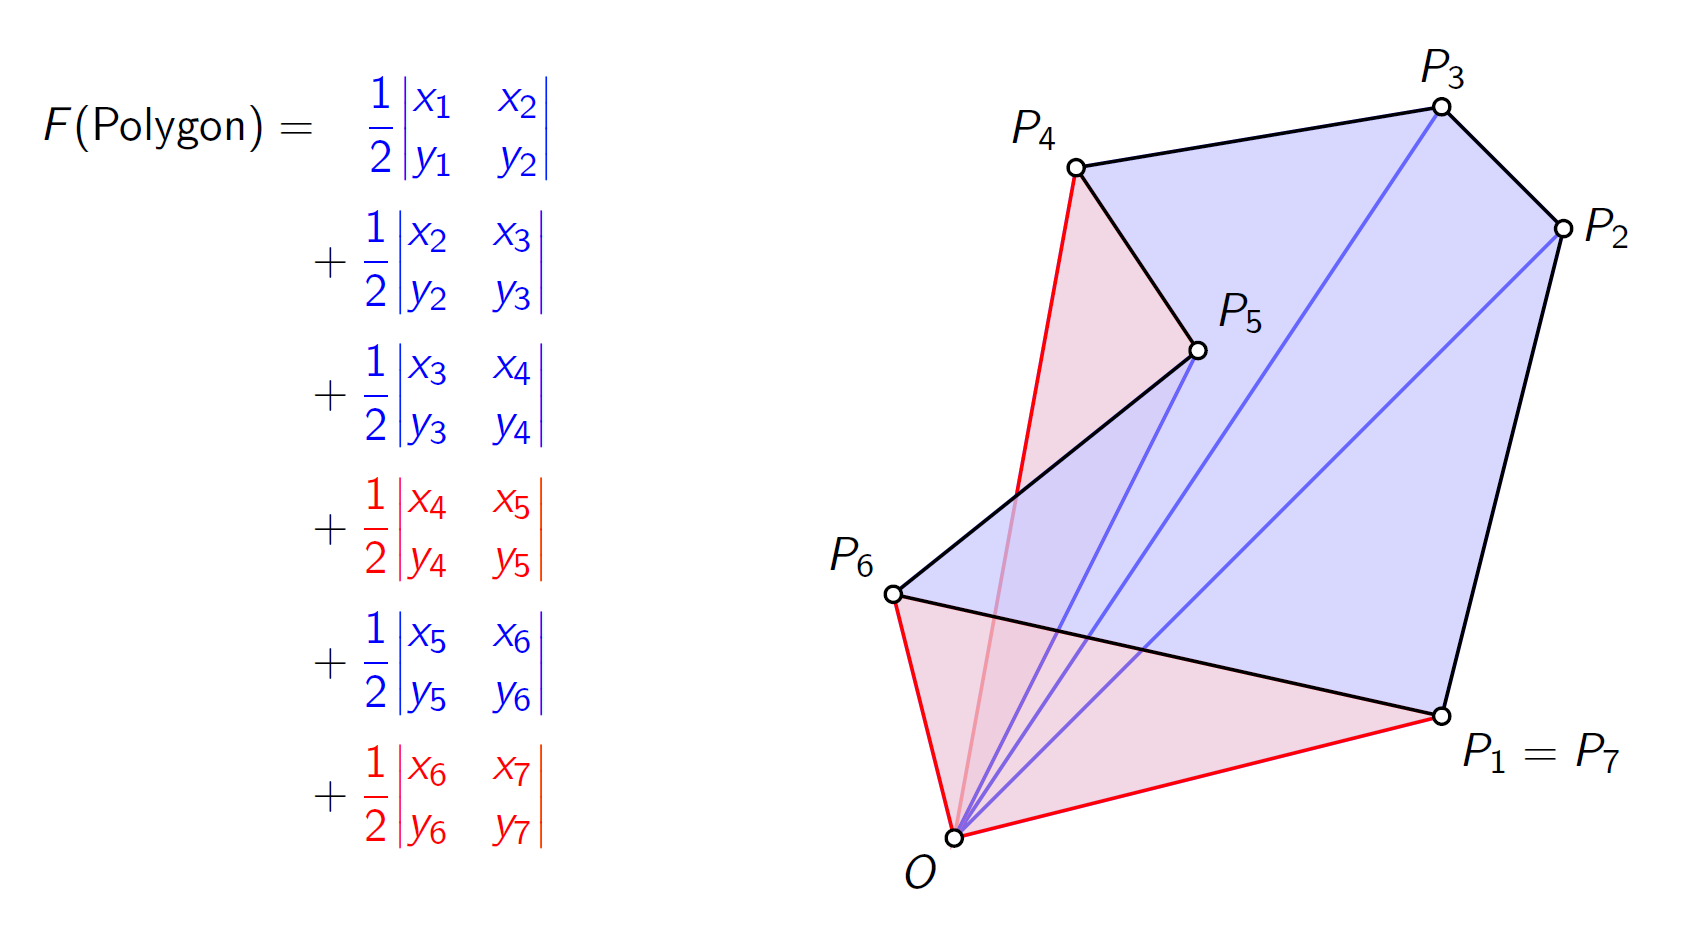
\includegraphics[width=\linewidth]{Bilder/flaeche-polygon} \\
		    \end{minipage}
		    \hfill
		    \begin{minipage}{0.48\linewidth}
		    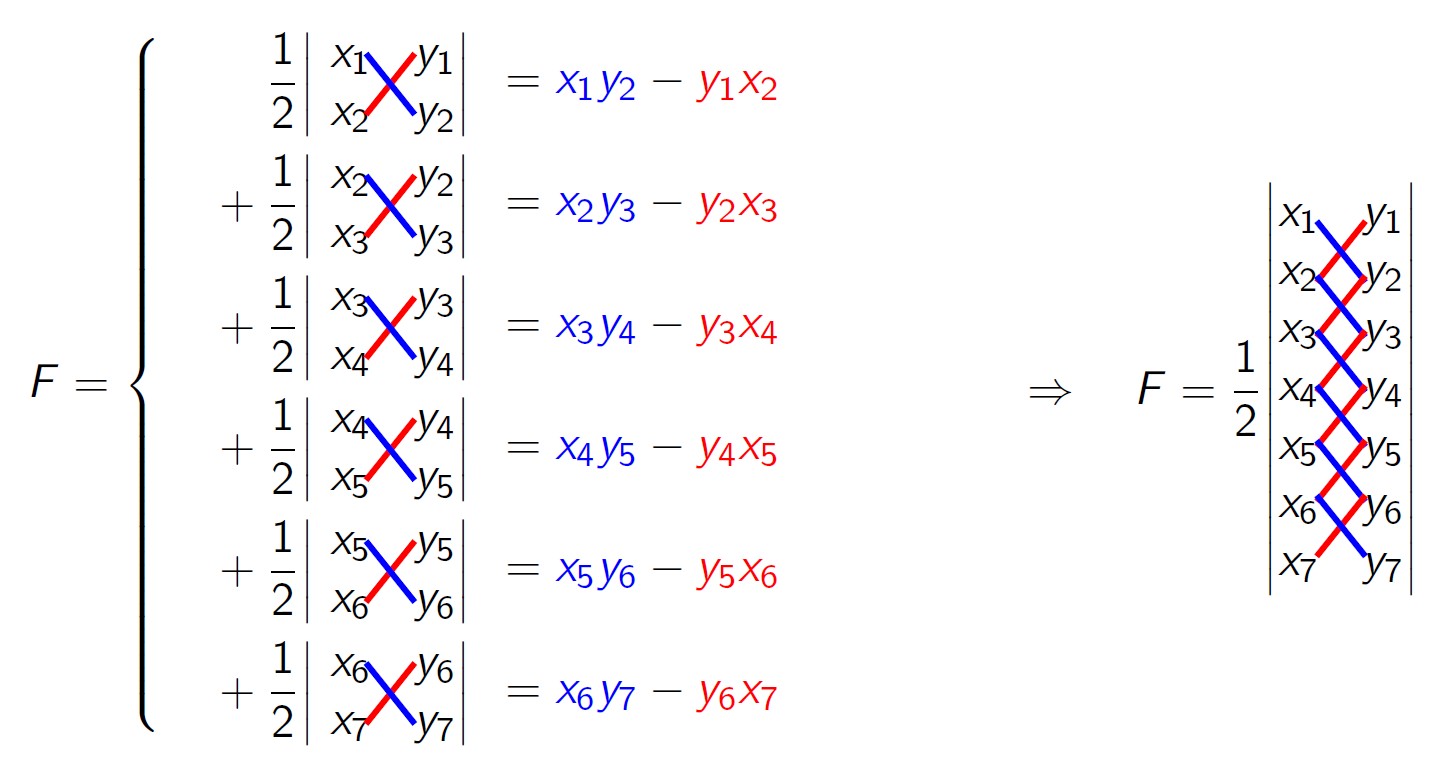
\includegraphics[width=\linewidth]{Bilder/schuhbaendel}
		    \end{minipage}

		    
		    \vfill\null
		    \columnbreak


		    

		    
			\subsection{Allgemeine Lösung für Schnittprobleme}	
			Um ein Schnittproblem zu lösen kann alles in ein Gauss-Tableau \\
			geschrieben werden, welches anschliessend gelöst werden kann. \\
			\\
			\begin{tabular}{ll}
			$E$ & Einheitsmatrix  \\ 
			$\vec{u}, \vec{v}$ & Richtungsvektoren \\
			$\vec{p_1}, \vec{p_1} $ & Stützvektoren \\
			\end{tabular}
			
			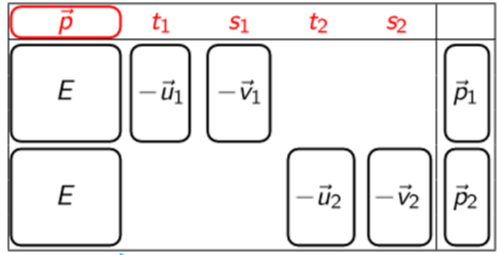
\includegraphics[width=0.7\linewidth]{Bilder/schnittpunkt-tableau} 
			
			
			\subsubsection{Beispiel: Schnittpunkt von zwei Geraden}
			
			
		$\textcolor{blue}{\begin{pmatrix} x_1 \\ x_2 \\ x_3 \end{pmatrix} = \begin{pmatrix} 18 \\ -7 \\ 0 \end{pmatrix} + s \cdot \begin{pmatrix} 7 \\ -2 \\ 1\end{pmatrix}}$ \qquad $\textcolor{orange}{\begin{pmatrix} x_1 \\ x_2 \\ x_3 \end{pmatrix} = \begin{pmatrix} -18 \\ 19 \\ 7 \end{pmatrix} + t \cdot \begin{pmatrix} -3 \\ 4 \\ 2\end{pmatrix}}$ \\
		
		\vspace{0.2cm}
		
		\begin{minipage}[b]{.5\linewidth} 
  		\begin{tabular}{| c c c c c | c |}
		\hline
		$x_1$ & $x_2$ & $x_3$ & $s$ & $t$ & \\
		\hline
		\textcolor{blue}1 & \textcolor{blue}0 & \textcolor{blue}0 & \textcolor{blue}{-7} & \textcolor{blue}0 & \textcolor{blue}{18} \\
		\textcolor{blue}0 & \textcolor{blue}1 & \textcolor{blue}0 & \textcolor{blue}2 & \textcolor{blue}0 & \textcolor{blue}{-7} \\
		\textcolor{blue}0 & \textcolor{blue}0 & \textcolor{blue}1 & \textcolor{blue}{-1} & \textcolor{blue}0 & \textcolor{blue}0 \\
		\textcolor{orange}1 & \textcolor{orange}0 & \textcolor{orange}0 & \textcolor{orange}0 & \textcolor{orange}3 & \textcolor{orange}{-18} \\
		\textcolor{orange}0 & \textcolor{orange}1 & \textcolor{orange}0 & \textcolor{orange}0 & \textcolor{orange}{-4} & \textcolor{orange}{19} \\
		\textcolor{orange}0 & \textcolor{orange}0 & \textcolor{orange}1 & \textcolor{orange}0 & \textcolor{orange}{-2} & \textcolor{orange}7 \\
	    \hline
		\end{tabular}		
  		\end{minipage}
		\hfill
		\begin{minipage}[b]{.45\linewidth} 
  		\begin{tabular}{| c c c c c | c |}
		\hline
		$x_1$ & $x_2$ & $x_3$ & $s$ & $t$ & \\
		\hline
		1 & 0 & 0 & 0 & 0 & -3 \\
		0 & 1 & 0 & 0 & 0 & -1 \\
		0 & 0 & 1 & 0 & 0 & -3 \\
		0 & 0 & 0 & 1 & 0 & -3 \\
		0 & 0 & 0 & 0 & 1 & -5 \\
		0 & 0 & 0 & 0 & 0 & 0 \\
	    \hline
		\end{tabular}		
		\end{minipage}		
		
		\vspace{0.2cm}
		
		Schnittpunkt: ($-3$ $\vert$ $-1$ $\vert$ $-3$) \quad $s = -3$ \quad $t = -5$	
		
		
		
		
		\subsubsection{Beispiel: Durchstosspunkt Gerade durch Ebene}
		    
		 $\textcolor{blue}{\begin{pmatrix} x_1 \\ x_2 \\ x_3 \end{pmatrix} = \begin{pmatrix} 0 \\ 0 \\ 1 \end{pmatrix} + s \cdot \begin{pmatrix} 1 \\ 1 \\ -1\end{pmatrix}}$ \quad $\textcolor{orange}{\begin{pmatrix} x_1 \\ x_2 \\ x_3 \end{pmatrix} = \begin{pmatrix} 0 \\ 0 \\ 0 \end{pmatrix} + u \cdot \begin{pmatrix} 1 \\ 0 \\ 1\end{pmatrix} + v \cdot \begin{pmatrix} 0 \\ 1 \\ 1\end{pmatrix}}$ \\
		\\

  		\begin{tabular}{| c c c c c c | c |}
		\hline
		$x_1$ & $x_2$ & $x_3$ & $s$ & $u$ & $v$ & \\
		\hline
		\textcolor{blue}1 & \textcolor{blue}0 & \textcolor{blue}0 & \textcolor{blue}{-1} & \textcolor{blue}0 & \textcolor{blue}0 &  \textcolor{blue}0 \\
		\textcolor{blue}0 & \textcolor{blue}1 & \textcolor{blue}0 & \textcolor{blue}{-1} & \textcolor{blue}0 & \textcolor{blue}0 &  \textcolor{blue}0 \\
		\textcolor{blue}0 & \textcolor{blue}0 & \textcolor{blue}1 & \textcolor{blue}1 & \textcolor{blue}0 & \textcolor{blue}0 &  \textcolor{blue}1 \\
		\textcolor{orange}1 & \textcolor{orange}0 & \textcolor{orange}0 & \textcolor{orange}0 & \textcolor{orange}{-1} & \textcolor{orange}0 & \textcolor{orange}0 \\
		\textcolor{orange}0 & \textcolor{orange}1 & \textcolor{orange}0 & \textcolor{orange}0 & \textcolor{orange}0 & \textcolor{orange}{-1} & \textcolor{orange}0 \\
		\textcolor{orange}0 & \textcolor{orange}0 & \textcolor{orange}1 & \textcolor{orange}0 & \textcolor{orange}{-1} & \textcolor{orange}{-1} & \textcolor{orange}0 \\
	    \hline
		\end{tabular}		


  		\begin{tabular}{| c c c c c c | c |}
		\hline
		$x_1$ & $x_2$ & $x_3$ & $s$ & $u$ & $v$ & \\
		\hline
		1 & 0 & 0 & 0 & 0 & 0 & $\frac{1}{3}$ \\
		0 & 1 & 0 & 0 & 0 & 0 & $\frac{1}{3}$ \\
		0 & 0 & 1 & 0 & 0 & 0 & $\frac{2}{3}$ \\
		0 & 0 & 0 & 1 & 0 & 0 & $\frac{1}{3}$ \\
		0 & 0 & 0 & 0 & 1 & 0 & $\frac{1}{3}$ \\
		0 & 0 & 0 & 0 & 0 & 1 & $\frac{1}{3}$\\
	    \hline
		\end{tabular}		
	
	\vspace{0.2cm}
	
		Durchstosspunkt: ($\frac{1}{3} \vert \frac{1}{3} \vert \frac{2}{3}$) \quad $s = \frac{1}{3}$ \quad $u = \frac{1}{3}$ \quad $v =  \frac{1}{3}$	
						
	
	
	
			\subsubsection{Beispiel: Schnittgerade von 2 Ebenen}		    					$\textcolor{blue}{\begin{pmatrix} x_1 \\ x_2 \\ x_3 \end{pmatrix} = \begin{pmatrix} 6 \\ 4 \\ 7 \end{pmatrix} + s \cdot \begin{pmatrix} 3 \\ -2 \\ 2\end{pmatrix} + t \cdot \begin{pmatrix} -5 \\ 3 \\ -7\end{pmatrix}}$ \\
			
			\vspace{0.2cm}
			
			 $\textcolor{orange}{\begin{pmatrix} x_1 \\ x_2 \\ x_3 \end{pmatrix} = \begin{pmatrix} 2 \\ 2 \\ 4 \end{pmatrix} + u \cdot \begin{pmatrix} 4 \\ 11 \\ 0\end{pmatrix} + v \cdot \begin{pmatrix} -1 \\ 1 \\ 3\end{pmatrix}}$ \\
		\\

  		\begin{tabular}{| c c c c c c c | c |}
		\hline
		$x_1$ & $x_2$ & $x_3$ & $s$ & $t$ & $u$ & $v$ &  \\
		\hline
		\textcolor{blue}1 & \textcolor{blue}0 & \textcolor{blue}0 & \textcolor{blue}{-3} & \textcolor{blue}5 & \textcolor{blue}0 & \textcolor{blue}0 & \textcolor{blue}6\\
		\textcolor{blue}0 & \textcolor{blue}1 & \textcolor{blue}0 & \textcolor{blue}2 & \textcolor{blue}{-3} & \textcolor{blue}{0} & \textcolor{blue}0 & \textcolor{blue}4\\
		\textcolor{blue}0 & \textcolor{blue}0 & \textcolor{blue}1 & \textcolor{blue}{-2} & \textcolor{blue}7 & \textcolor{blue}0 & \textcolor{blue}0 & \textcolor{blue}7 \\
		\textcolor{orange}1 & \textcolor{orange}0 & \textcolor{orange}0 & \textcolor{orange}0 & \textcolor{orange}0 & \textcolor{orange}{-4} & \textcolor{orange}1 & \textcolor{orange}2 \\
		\textcolor{orange}0 & \textcolor{orange}1 & \textcolor{orange}0 & \textcolor{orange}0 & \textcolor{orange}0 & \textcolor{orange}{-11} & \textcolor{orange}{-1} & \textcolor{orange}2 \\
		\textcolor{orange}0 & \textcolor{orange}0 & \textcolor{orange}1 & \textcolor{orange}0 & \textcolor{orange}0 & \textcolor{orange}0 & \textcolor{orange}{-3} & \textcolor{orange}4 \\
		\hline
		\end{tabular}		
 
  		\begin{tabular}{| c c c c c c c | c |}
		\hline
		$x_1$ & $x_2$ & $x_3$ & $s$ & $t$ & $u$ & $v$ & \\
		\hline
		1 & 0 & 0 & 0 & 0 & 0 & 1 & $\frac{10}{3}$\\
		0 & 1 & 0 & 0 & 0 & 0 & -1 & $\frac{17}{3}$\\
		0 & 0 & 1 & 0 & 0 & 0 & -3 & 4\\
		0 & 0 & 0 & 1 & 0 & 0 & 2 & $-\frac{1}{3}$\\
		0 & 0 & 0 & 0 & 1 & 0 & 1 & $\frac{1}{3}$\\
		0 & 0 & 0 & 0 & 0 & 1 & 0 & $\frac{1}{3}$\\
		\hline
		\end{tabular}		
		
		\vspace{0.2cm}

		Schnittgerade: $\begin{pmatrix} x_1 \\ x_2 \\ x_3 \end{pmatrix} = \begin{pmatrix} \frac{10}{3} \\ \frac{17}{3} \\ 4 \end{pmatrix} + v \cdot \begin{pmatrix} -1 \\ 1 \\ 3 \end{pmatrix} $
		
		 
			
			\subsection{Orthonormalisierung}
			Beschreibt, wie man von einer beliebigen Basis zu einer \\			
			Orthonormalbasis kommt \\		
			Orthonormalbasis: siehe Abschnitt 4.4 \\
			
			
			\subsubsection{Gram-Schmidtsches Orthonormalisierungsverfahren}
			Basisvektoren $\vec{a_1}$, $\vec{a_2}$ und $\vec{a_3}$ sind nicht orthagonal. Sie sollen \\
			orthagonalisiert werden und durch die Vektoren $\vec{b_1}$, $\vec{b_2}$ und $\vec{b_3}$ \\
			ausgedrückt werden: \\
			
			\begin{tabular}{ll}
			$\vec{b_1}$ = $\frac{\vec{a_1}}{\vert \vec{a_1} \vert}$ & $\vec{b_2}$  = $\frac{\vec{a_2} - ( \vec{a_2} \bullet \vec{b_1} ) \vec{b_1}}{\vert \vec{a_2} - ( \vec{a_2} \bullet \vec{b_1} ) \vec{b_1} \vert}$\\
		 \\
			$\vec{b_3}$ = $\frac{\vec{a_3} - ( \vec{a_3} \bullet \vec{b_1} ) \vec{b_1} - ( \vec{a_3} \bullet \vec{b_2} ) \vec{b_2}}  {\vec{a_3} - ( \vec{a_3} \bullet \vec{b_1} ) \vec{b_1} - ( \vec{a_3} \bullet \vec{b_2} ) \vec{b_2}}$  &  kann beliebig weitergeführt werden \\
			\\
			\end{tabular}
					
					
			\vfill\null
			\columnbreak			
			
			
			\subsection{Least Squares Überbestimmtes Gleichungssystem}
			Ein Gleichungssystem mit mehr Gleichungen als Unbekannten ist im allgemeinen nicht lösbar \\	
			Wir suchen also eine Lösung, welche am ''wenigsten falsch'' ist bzw. $\vert A \cdot \vec{x} - \vec{b} \vert$ möglichst klein 
				
			\subsubsection{Beispiel Least Squares}
			Die Unbekannten sind \textcolor{red}{rot} eingefärbt \\
			\\
			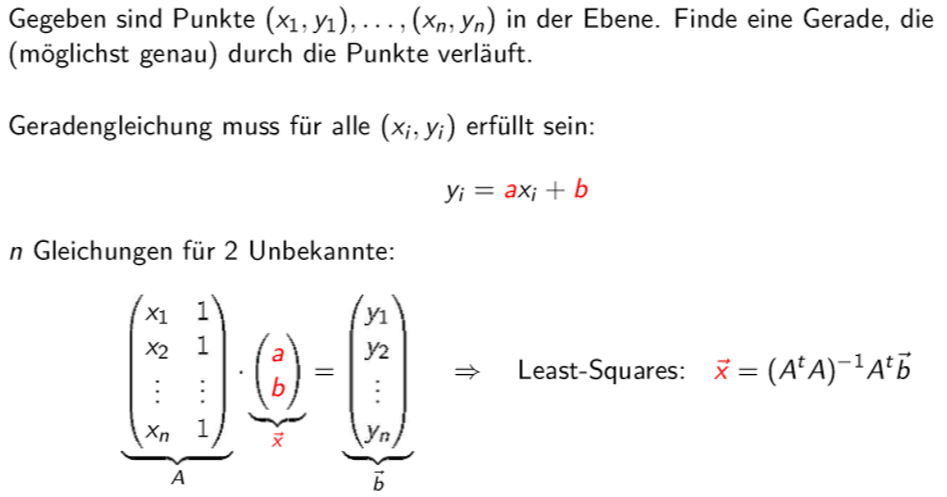
\includegraphics[width=0.8\linewidth]{Bilder/least-squares}\\
			\\
			\textbf{nichtlineare Teile (z.B. $d^2$) können einfach neu benannt weden ($d^2 = m$) und in das Verfahren eingesetzt werden.} \\
			Sobald eine lineare Lösung gefunden ist kann der nichtlineare Teil berechnet werden.
			
			
			\subsection{Kreis und Kugel}		
			
			\subsubsection{Kreis}
			\begin{tabular}{ll}
			Vektorgleichung: & $(\vec{p} - \vec{m})^2 = r^2$\\
			Koordinatengleichung: & $(x- m_x)^2 + (y-m_y)^2 = r^2$\\
			\\
			\end{tabular}
			
			Die Koeffizienten von $x$ und $y$ entsprechen Koordinatenmittelpunkt: \\
			$x^2 - 2 \textcolor{red}{m_x} x + m_x^2 + y^2 - 2 \textcolor{red}{m_y} y + m_y^2 = r^2 $		\\
			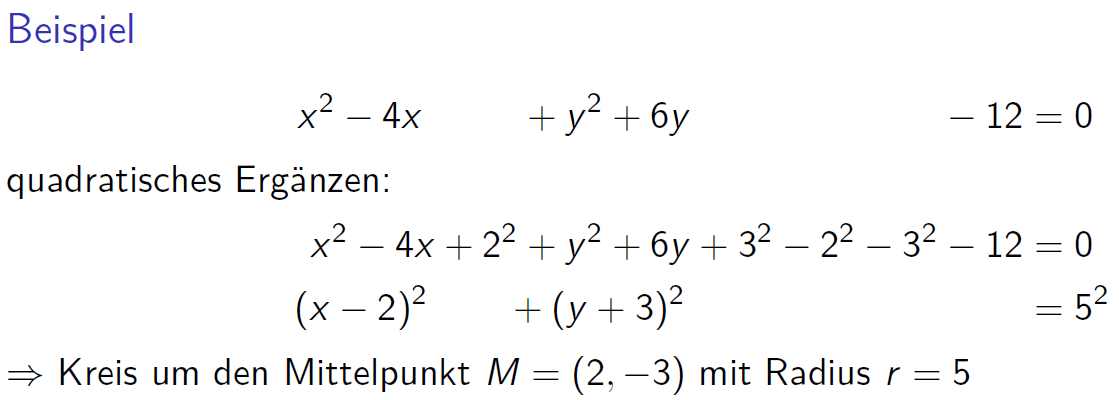
\includegraphics[width=0.8\linewidth]{Bilder/kreisgleichung}	\\
			
			\subsubsection{Thales-Kreis}
			\begin{minipage}[b]{.45\linewidth} 
  			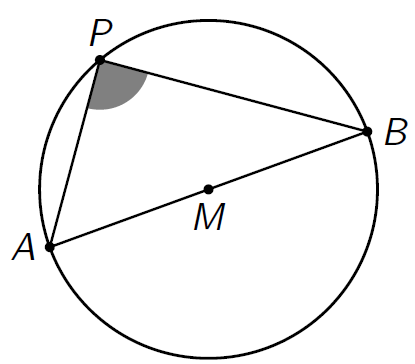
\includegraphics[width=0.7\linewidth]{Bilder/thales-kreis}
			\end{minipage}
			\hfill
			\begin{minipage}[b]{.5\linewidth} 
  			Thales-Kreis: \\
  			\\
  			$\left( \vec{p} - \frac{\vec{a} + \vec{b}}{2} \right) ^2 = \left( \frac{\vec{a} - \vec{b}}{2} \right) ^2 = r^2$	\\
  			\\
  			\\
			\end{minipage}		
			
			\vfill\null
			\columnbreak			
			
			
			\subsubsection{Durchstosspunkt Gerade-Kreis}
				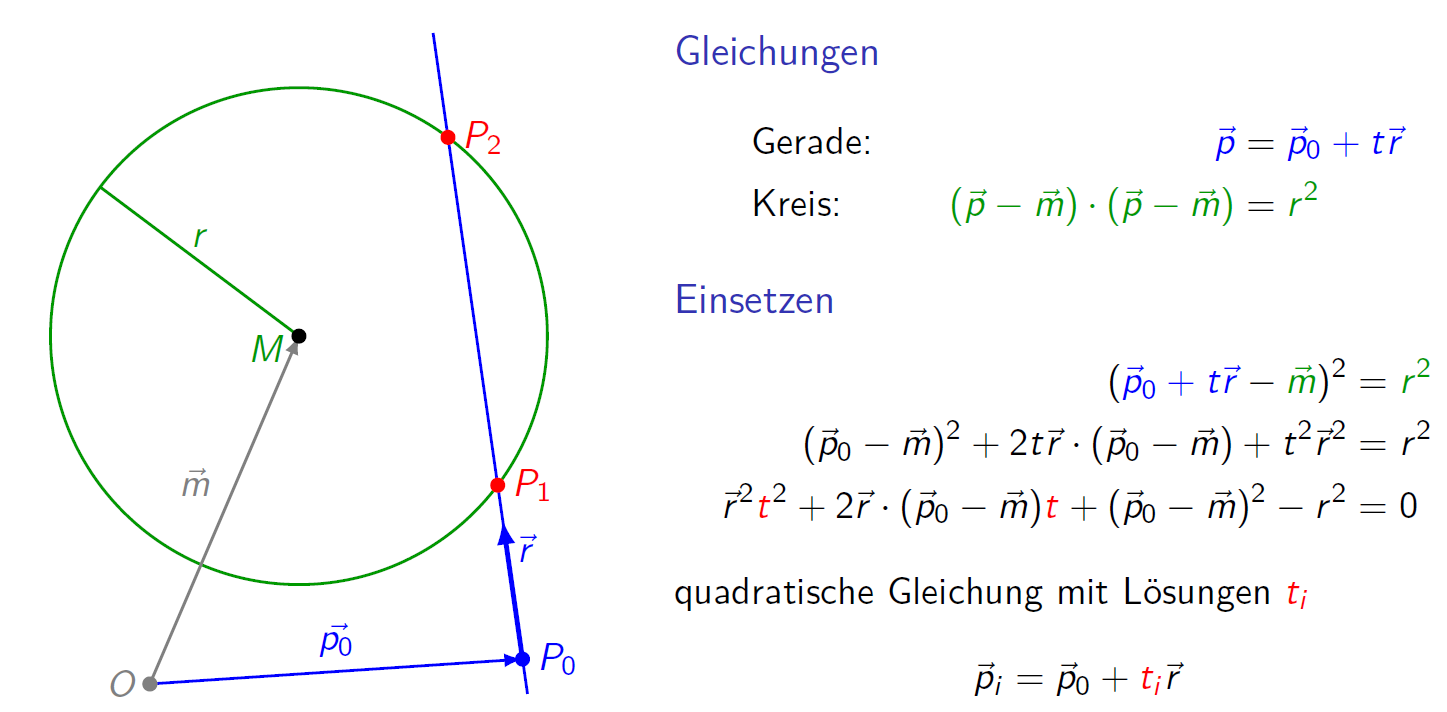
\includegraphics[width=0.8\linewidth]{Bilder/durchstosspunkt-gerade-kreis}	
			
			\subsubsection{Tangente an Kreis}
			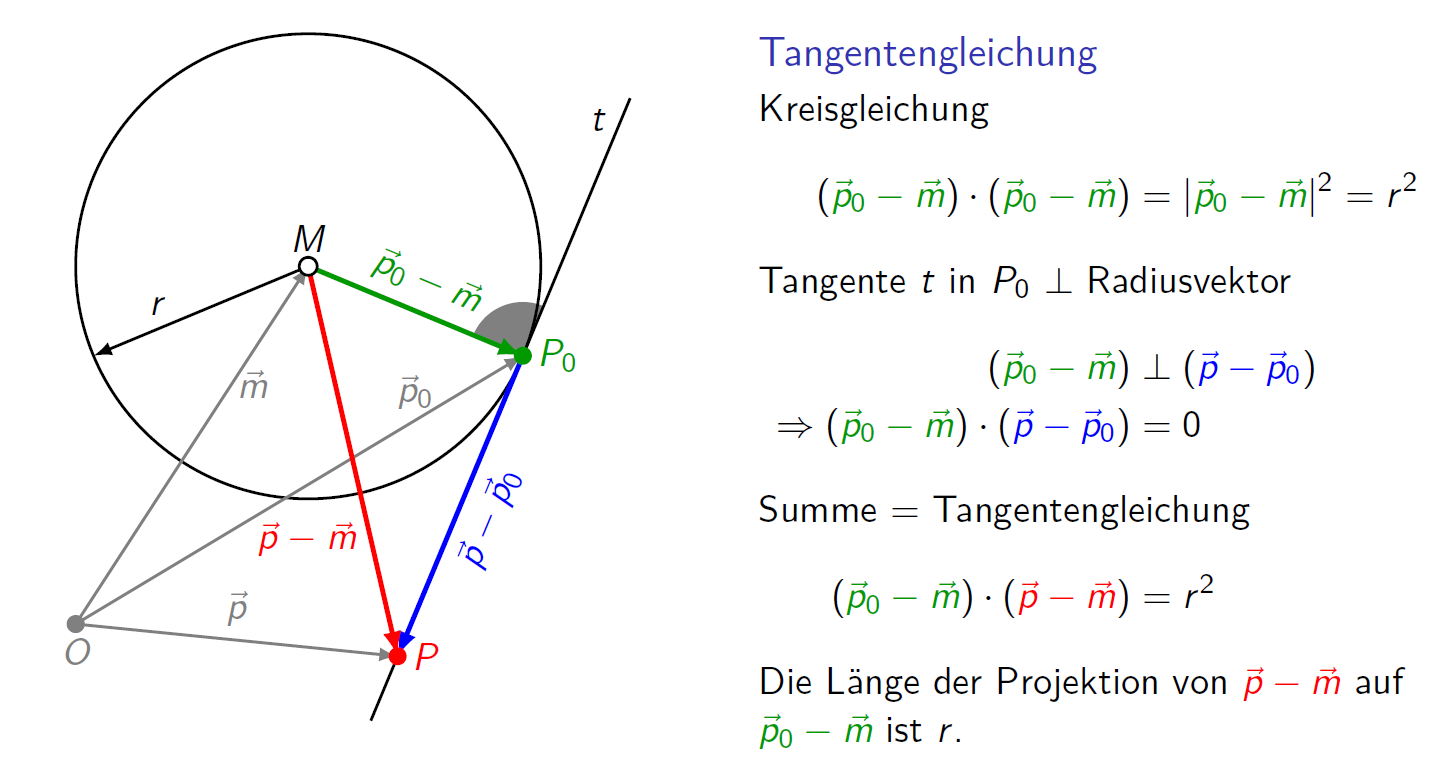
\includegraphics[width=0.8\linewidth]{Bilder/kreis-tangente}	
			
			
			\subsubsection{Kugel}
			\begin{tabular}{ll}
			Vektorgleichung: & $(\vec{p} - \vec{m})^2 = r^2$\\
			Koordinatengleichung: & $(x - m_x)^2 + (y - m_y)^2 + (z - m_z)^2 = r^2$\\
			\end{tabular}
			
			\subsubsection{Zusammenfassung Kugel}
			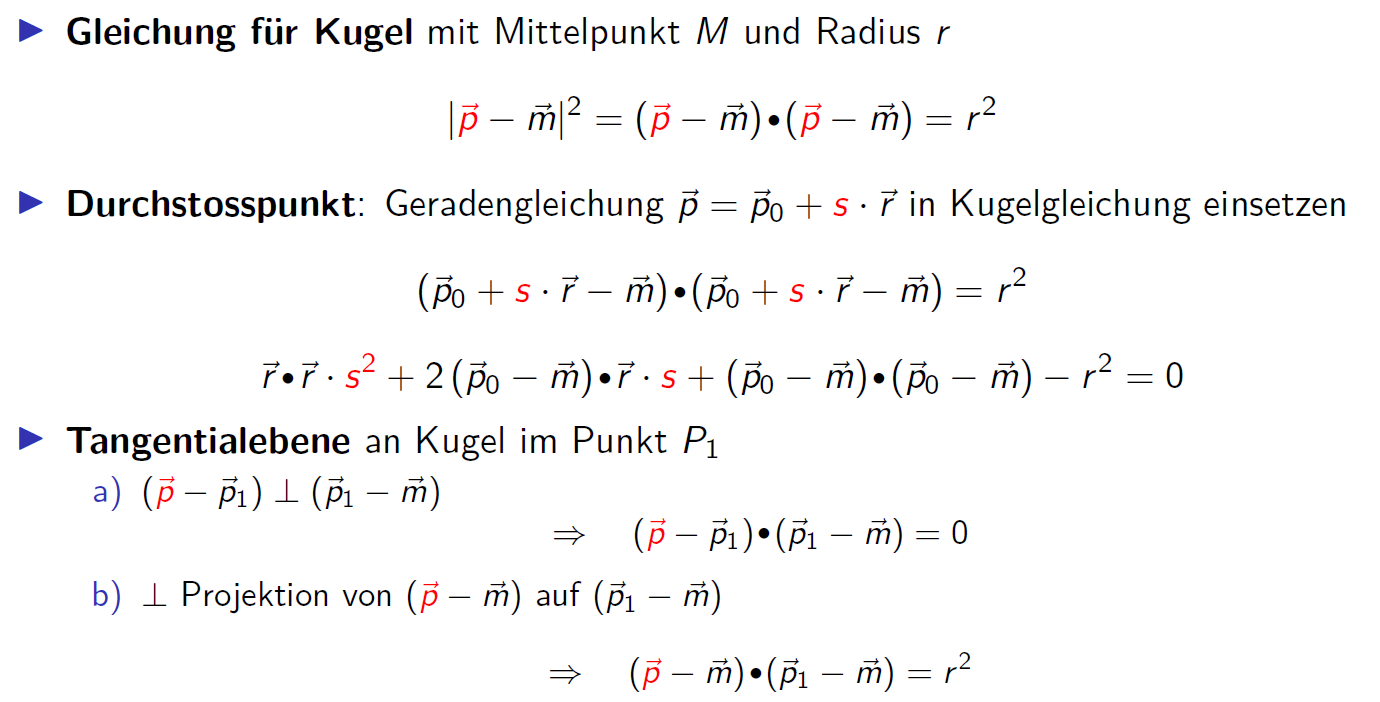
\includegraphics[width=0.8\linewidth]{Bilder/kugel}	
			
			
			\vfill\null
			\columnbreak	
			
			
			
			\subsection{Abstandsprobleme}
		
		\subsubsection{Abstand Punkt-Ebene}
		Berechnung mittels Hessescher Normalform 
		
		
		\subsubsection{Abstand Punkt-Gerade}
		Der Abstand $h$ zwischen der Geraden $g$ und dem Punkt $Q$ entspricht dem Lot zur Geraden $g$ durch $Q$ \\
		Gerade in Paramterdarstellung: $\vec{p} = \vec{p_0} + t \vec{r}$ \\
		 
		 \begin{minipage}{0.45\linewidth}
		 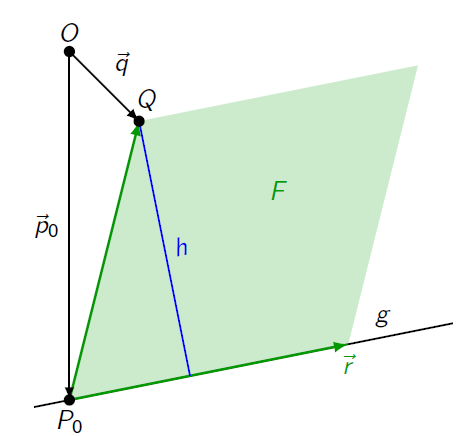
\includegraphics[width=0.6\linewidth]{Bilder/punkt-gerade}
		 \end{minipage}
		\hfill
		\begin{minipage}{0.45\linewidth}
		 $$h = \frac{F}{\vline \vec{r} \vline} =  \frac{r \times ( \vline \vec{q} - \vec{p_0} \vline )}{\vline \vec{r} \vline} $$
		 \end{minipage}

			\subsubsection{Abstand windschiefer Geraden in 3D} 
			Zwei Geraden in Parameterdarstellung:\\					$\vec{p} = \vec{p_0} + t \vec{r_1}$ und $\vec{q} = \vec{q_0} + 2 \vec{r_2}$ \\
			die sich nicht schneiden und nicht parallel sind \\
			
		Abstand $d = (\vec{q_0} -\vec{p_0}) \bullet \frac{\vec{r_1} \times \vec{r_2}}{\vert \vec{r_1} \times \vec{r_2} \vert} $
		
		
		\subsubsection{Minimaler Abstand}
			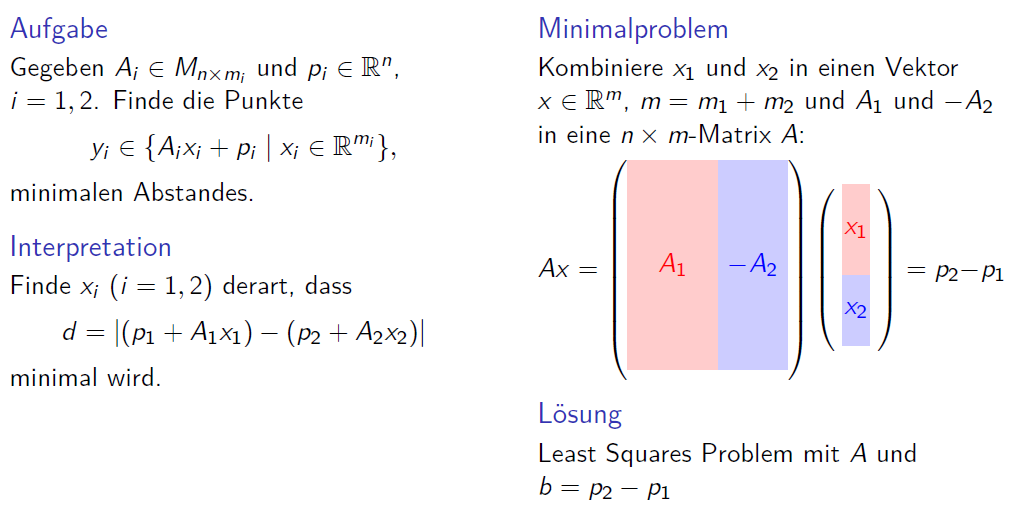
\includegraphics[width=0.9\linewidth]{Bilder/minimaler-abstand}	
		
		
		\vfill\null
		\columnbreak	
		
		
		 \section{Eigenwerte / Eigenvektoren}   
		 Ein Vektor $\vec{v}$ heisst Eigenvektor der $n \times n$ Matrix A zum \\
		 Eigenwert $\lambda$, wenn 
		$$A \vec{v} = \lambda \vec{v} \quad \text{und} \quad \vec{v \neq 0}$$
		\\
		\textbf{Eigenschaften}\\
		\begin{tabular}{ll}
		$\bullet$ & Ein Eigenvektor $\vec{v}$ wird durch die Matrix A nur gestreckt \\
		& (Streckungsfaktor $\lambda$) \\
		$\bullet$ & Es gibt maximal n verschiedene Eigenwerte $\lambda$ \\
		$\bullet$ & Zu jedem Eigenwert gibt es unendlich viele Eigenvektoren \\
		\end{tabular}		 
		 
	 
	 
		 \textbf{Eigenwerte und Eigenvektoren finden} \\
		 \begin{tabular}{ll}
		1. & Eigenwertproblem: $A \textcolor{red}{\vec{v}} = \textcolor{red}{\lambda \vec{v}}$ $\Rightarrow$  $(A - \lambda E) \vec{v} = 0$  \\
		2. & Charakteristische Gleichung: $\det(A -  \textcolor{red}{\lambda} E) = 0$ \\
		3. & Berechnung der Eigenwerte \textcolor{red}{$\lambda_i$} als Lösungen der \\
		& charakteristischen Gleichung \\
		4. & Berechnung der Eigenvektoren \textcolor{red}{$\vec{v_i}$} mittels Gauss-Algorithmus: \\
		& $(A - \lambda_i E) \vec{v_i} = 0$ \\
		5. & Resultat kontrollieren: $A \vec{v_i} = \lambda_i \vec{v_i}$ \\
		\\
		\end{tabular}		 
		
		
		Hinweis: Wenn $AA^t$ oder $A^tA$	eine Zeile und Spalte mit nur\\
		einem Zahleneintrag enthalten, so ist die Zahl ein Eigenwert zum \\
		zugehörigen Standardbasisvektor. \\
		Die weiteren EW und EV können ohne diese Zeile/Spalte berechnet werden!	   
			
			
			\subsection{Eigenschaften der Matrix A bzgl. Eigenwerte}
			\begin{tabular}{ll}
			$\bullet$ & Spur($A$) = Spur($A'$) = Summe der Eigenwerte von $A$ \\
			$\bullet$ & $\det(A) = \det(A')$ = Produkt aller Eigenwerte von $A$\\
			\\
			\end{tabular}
			
			\begin{minipage}{0.35\linewidth}
			$AA^t = \begin{pmatrix} 2 & 0 & -2 \\ 0 & 9 & 0 \\ -2 & 0 & 2 \end{pmatrix}$ \\
			\\
			$A_0 = \begin{pmatrix}2 & -2 \\ -2 & 2 \end{pmatrix}$						
			
			\end{minipage}	
			\hfill
			\begin{minipage}{0.55\linewidth}
			
			Aus $AA^t$ kann man $\lambda = 9$ direkt ablesen. \\
			
			Daraus folgt: $\vec{v_{\lambda}} = \begin{pmatrix} 0 \\ 1 \\ 0 \end{pmatrix}$	
			\end{minipage}					   
		   
		   
		   
		   
		   
				\subsubsection{Beispiel Eigenwerte und Eigenvektoren berechnen}
		 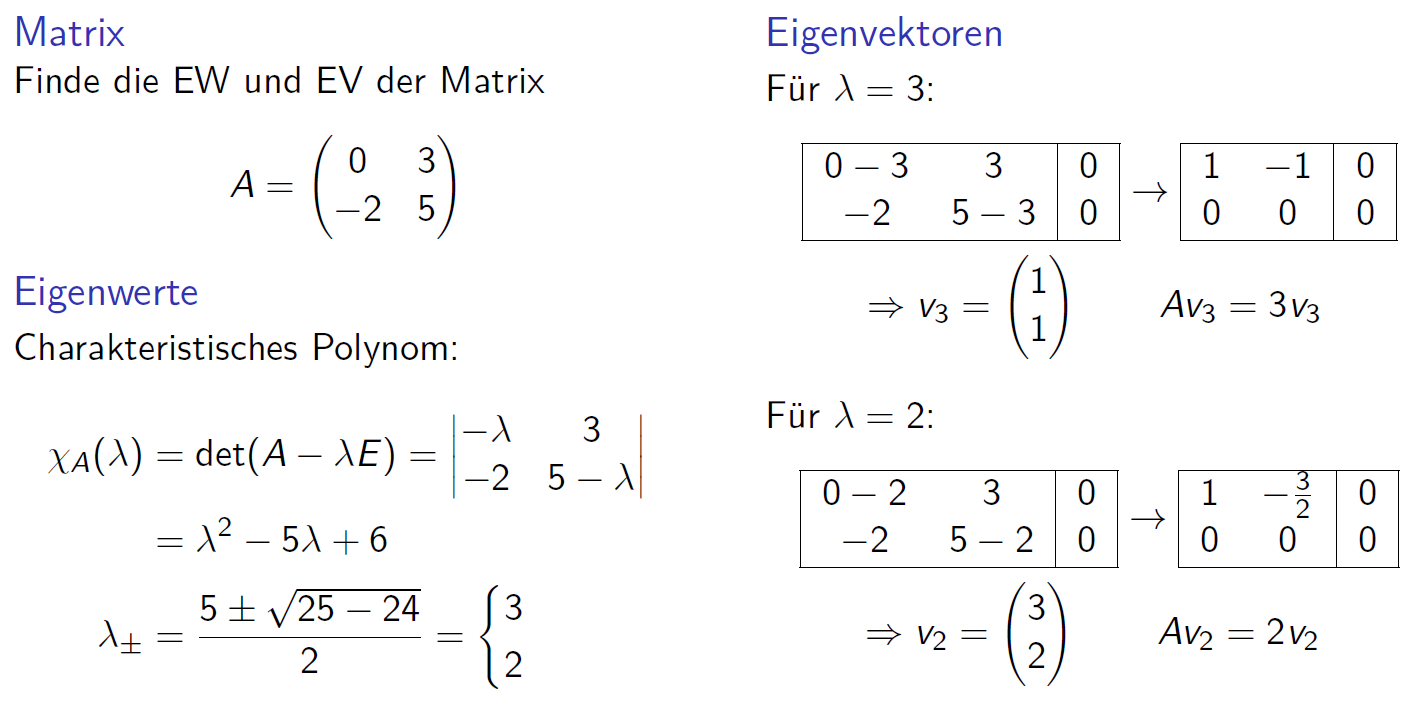
\includegraphics[width=0.85\linewidth]{Bilder/eigenwerte-eigenvektoren} \\
		 
			\textbf{Rechenregeln für Eigenwerte}
			$\frac{1}{\lambda} = \lambda - 1$ \\		 
		 
		 
		 \vfill\null
		 \columnbreak
		 
		 
		 
		 
		 
		 
		   \subsection{Diagonalisierung einer Matrix}
			Mit Diagonalmatritzen kann man einfach rechnen \\	
			\\
			\textbf{Eine Matrix ist diagonalisierbar, wenn:} \\
			\begin{tabular}{ll}
			$\bullet$ & Die Matrix symmetrisch ist , also $A = A^t$\\
			$\bullet$ & \textbf{Eine Basis aus Eigenvektoren existiert} \\
			\end{tabular}				    
			
			\subsubsection{Vorgehen Matrix diagonalisieren} 
		 \begin{tabular}{ll}
		1. & Eigenbasis $C$ aus n linear unabh. Eigenvektoren finden  \\
		& Spalten von $C$ sind Eigenvektoren\\
		2. & Basis-Transformationsmatrix $T$ berechnen \\
		& $T = C^{-1}$ $\rightarrow$ Matrix aus Eigenvektoren invertieren \\
		3. & Diagonalisierte Matrix $A'$ berechnen \\
		& $A' = T A T^{-1}$ $\rightarrow$ $A$' enhält Eigenwerte auf Diagonalen \\
		\end{tabular}		 
		 
		  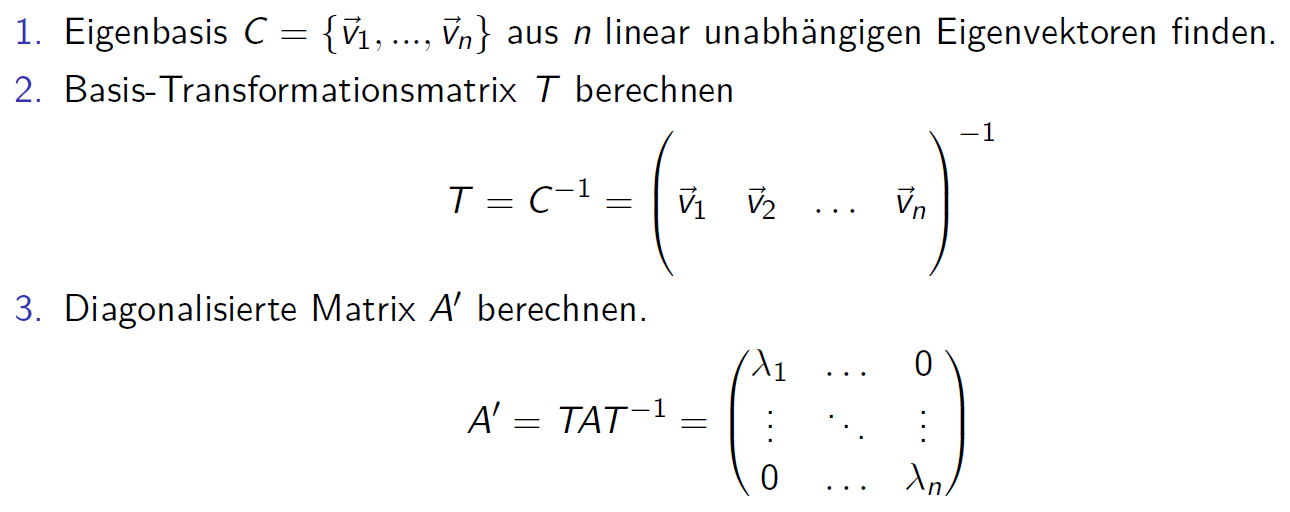
\includegraphics[width=0.7\linewidth]{Bilder/matrix-diagonalisieren} \\ 
			
			
			

			\subsubsection{Transofotmationsmatrix $T$; Eigenbasis $C$}
			\begin{tabular}{ll}
			$\bullet$ & Die Eigenbasisis-Matrix $C$ enthält in ihren Spalten die \\
			& Eigenvektoren der Matrix $A$ (Anfangsmatrix) \\
			$\bullet$ & Die Transformationsmatrix $T$ ist die Inverse von $C$ \\
			\end{tabular}
			
			\subsubsection{Spezialfall Symmetrische Matrix diagonalisieren}
		    
			Die Eigenvektoren einer symmetischen Matrix sind orthagonal \\
		   
		   
		   \subsection{Singulärwertzerlegung (SVD)}
			Eine $m \times n$ Matrix $A$ wird zerlegt in zwei orthagonale Matritzen und eine Diagonalmatrix \\
			$A = U \, \Sigma \, V^t$	 \\	  
			\\
			\begin{tabular}{ll}
			$U$ & orthagonale $m \times m$ Matrix  ($U$ diagonalisiert $AA^t$)\\
			$V$ & orthagonale $n \times n$ Matrix ($V$ diagonalisiert $A^tA$)\\
			$V^t$ & Transponierte von $U$ \\
			$\Sigma$ & Diagnonalmatrix mit $r$ Singulärwerten $\sigma_0$ bis $\sigma_r$ \\
			\end{tabular}			 
		   
		   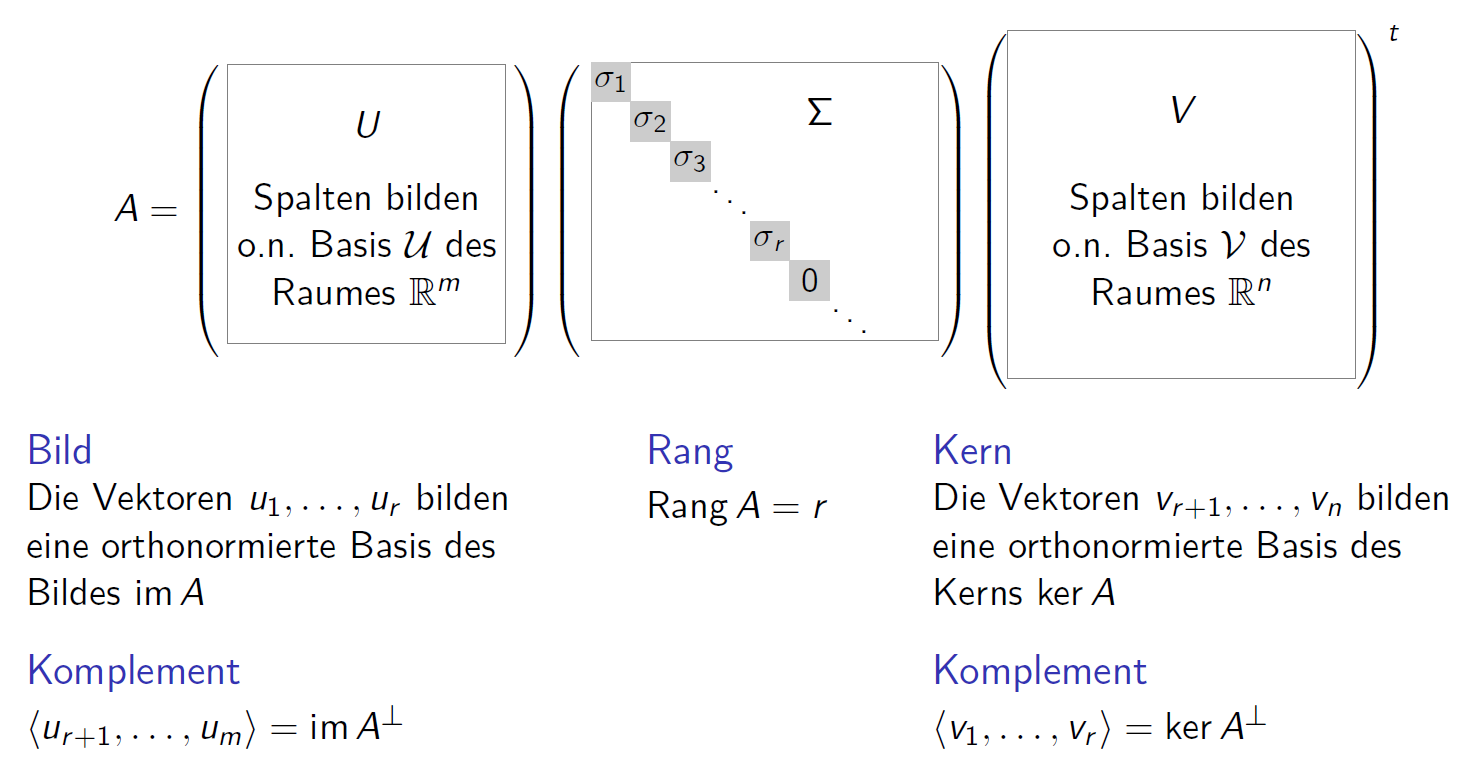
\includegraphics[width=0.65\linewidth]{Bilder/SVD} \\
		   
		   \vfill\null
			\columnbreak
		   
		   \subsubsection{Vorgehen Singulärwertzerlegung}
		   \begin{tabular}{ll}
		   1. & $AA^t$ und $A^tA$ berechnen \\
		   2. & Eigenwerte von $AA^t$ oder $A^tA$ berechnen (EW identisch) \\
		   3. & Eigenwerte der Grösse nach sortieren: $\sigma_1 \geq \sigma_2 \geq ... \geq \sigma_r \geq 0$\\
		   4. & $V$ = auf Länge 1 normierte Eigenvektoren von $A^tA$ \\
		   5. & $U$ = Spalten $u_i$ mit $u_i = \frac{A v_i}{\vert A v_i \vert}$ \\
		   6. & Singulärwerte bestimmen: $\sigma_i = \sqrt{\lambda_i}$ und Matrix $\Sigma$ füllen \\
		   7. & Kontrolle mit $A = U \, \Sigma \, V^t$ \\
		   \end{tabular}
		   
		   
			
	
			
			
		   \subsection{Pseudoinverse}
			\textbf{Die Pseudoinverse löst  Gleichungssysteme mit der Lösung minimaler Länge}		\\   
			$\vert x \vert$ ist minimal \\
		   
		     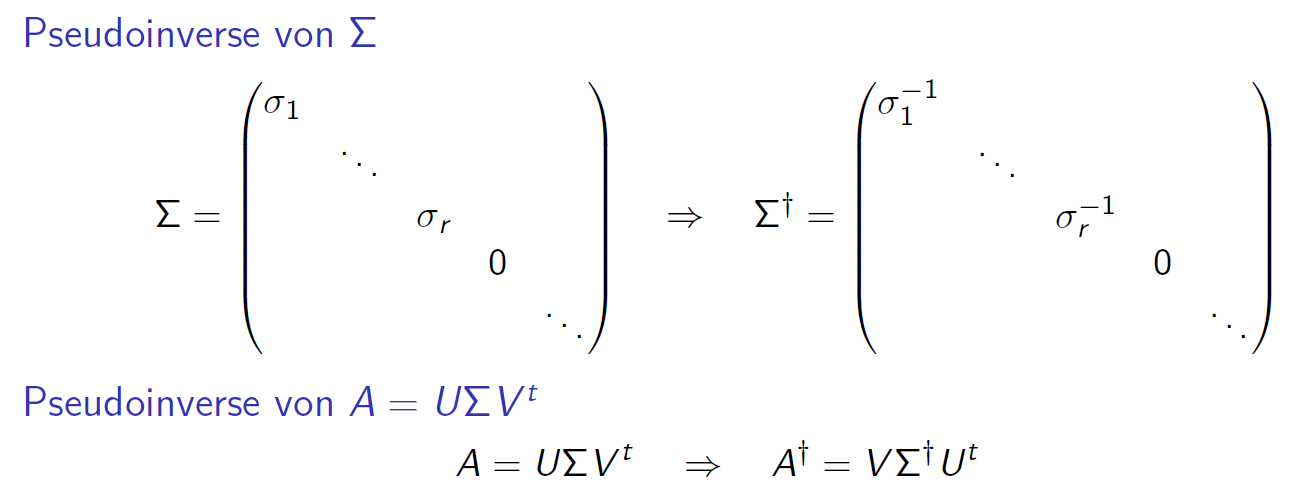
\includegraphics[width=0.8\linewidth]{Bilder/pseudoinverse} \\
		     
		    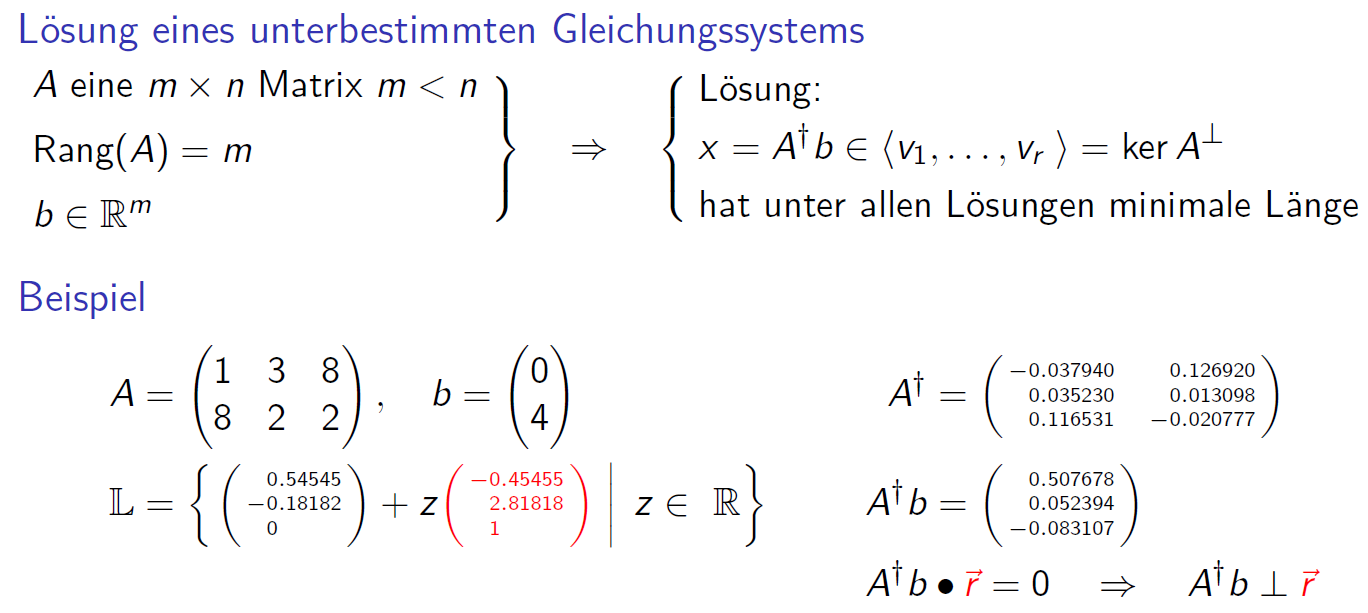
\includegraphics[width=0.8\linewidth]{Bilder/pseudoinverse2} \\
		    
		    
		    
		    
		 \section{Matritzenzerlegung}
		 Matritzen werden aus den folgenden Gründen zerlegt: \\
		 \begin{tabular}{ll}
		 $\bullet$ &  schwierige Matrix in einfachere Matritzen aufteilen \\
		 $\bullet$ & Vereinfachung schwieriger Berechnungen \\
		 & z.B. Eigenwertzerlegung $A = T^{-1} A' T$ \\
		 $\bullet$ & Verienfachte Berechnung der Determinanten 
		 \end{tabular}
		 
		 \vfill\null
		 \columnbreak
		 
		 
		    \subsection{LU-Zerlegung $(A = L \cdot U)$}
			Rechnung: \quad  $\det(A) =  \det(L) \cdot \det(U)$ \\ 
			$L$ = Matrix bestehnd aus Pivot-Spalten (oben rechts Nullen) \\
			$U$ = Diagonale mit 1en, oben rechts Elemente von Gauss ohne Rückwärts-Einsetzen, unten rechts Nullen \\	
			
			\subsubsection{Beispiel LU-Zerlegung}
			
			$A = \begin{pmatrix}	3 & 3 & -3 \\ -6 & -4 & 2 \\ 3 & 13 & -18 \end{pmatrix}$ \qquad $\rightarrow$ Gauss-Algorithmus durchführen \\
			\vspace{0.3cm}
			
			\begin{minipage}{0.25\linewidth}
			\begin{tabular}{|c c c|}
			\hline
			\textcolor{blue}3 & 3 & -3 \\
			\textcolor{blue}{-6} & -4 & 2 \\
			\textcolor{blue}3 & 13 & -18 \\
			\hline
			\end{tabular}
			\end{minipage}	
			\hfill
			\begin{minipage}{0.25\linewidth}
			\begin{tabular}{|c c c|}
			\hline
			1 & 1 & -1 \\
			0 & \textcolor{orange}2 & -4 \\
			0 & \textcolor{orange}{10} & -15 \\
			\hline
			\end{tabular}
			\end{minipage}		
			\hfill
			\begin{minipage}{0.25\linewidth}
			\begin{tabular}{|c c c|}
			\hline
			1 & 1 & -1 \\
			0 & 1 & -2 \\
			0 & 0 & \textcolor{green}5 \\
			\hline
			\end{tabular}
			\end{minipage}	
			
			\vspace{0.3cm}
			
			\begin{minipage}{0.25\linewidth}
			\begin{tabular}{|c c c|}
			\hline
			\textcolor{violet}1 & \textcolor{violet}1 & \textcolor{violet}{-1} \\
			0 & \textcolor{violet}1 & \textcolor{violet}{-2} \\
			0 & 0 & \textcolor{violet}1 \\
			\hline
			\end{tabular}
			\end{minipage}	
			\hfill
			\begin{minipage}{0.65\linewidth}
			$L = \begin{pmatrix} \textcolor{blue}3 & 0 & 0 \\ \textcolor{blue}{-6} & \textcolor{orange}2 & 0 \\ \textcolor{blue}3 & \textcolor{orange}{10} & \textcolor{green}5   \end{pmatrix}$ \quad $U = \begin{pmatrix} \textcolor{violet}1 & \textcolor{violet}1 & \textcolor{violet}{-1} \\ 0 & \textcolor{violet}1 & \textcolor{violet}{-2} \\ 0 & 0 & \textcolor{violet}1  
			 \end{pmatrix}$
			\end{minipage}				    
		    
		    
		    
		    
		    \subsection{LR-Zerlegung $(A = L' \cdot R)$}
		    Die LR-Zerlegung (bzw. L'R-Zerlegung)  entsteht aus der \\
		    LU-Zerlegung \\
		    
		    Rechnung: \quad  $\det(A) =  \det(L') \cdot \det(R)$ \\ 
			$L' = L D^{-1} $ \\
			$R = DU$ \\
			$D$ = Diagonalmatrix mit den Pivot-Elementen 
			
			
			\subsubsection{Beispiel LR-Zerlegung}
			Fortsetzung des Beispiels der LU-Zerlegung! \\
			\\
			$D = \begin{pmatrix} 3 & 0 & 0 \\ 0 & 2 & 0 \\ 0 & 0 & 5  \end{pmatrix}$ \quad $D^{-1} = \begin{pmatrix} \frac{1}{3} & 0 & 0 \\ 0 & \frac{1}{2} & 0 \\ 0 & 0 & \frac{1}{5}  \end{pmatrix}$ \\
			
			\vspace{0.3cm}
			
			$L' = L D^{-1} = \begin{pmatrix} 3 & 0 & 0 \\ -6 & 2 & 5 \\ 3 & 10 & 5   \end{pmatrix}  \begin{pmatrix} \frac{1}{3} & 0 & 0 \\ 0 & \frac{1}{2} & 0 \\ 0 & 0 & \frac{1}{5}  \end{pmatrix} = \begin{pmatrix} 1 & 0 & 0 \\ -2 & 1 & 0 \\ 1 & 5 & 1   \end{pmatrix}$ \\
			
			\vspace{0.3cm}
			
			$R = DU = \begin{pmatrix} 3 & 0 & 0 \\ 0 & 2 & 0 \\ 0 & 0 & 5  \end{pmatrix}  \begin{pmatrix} 1 & 1 & -1 \\ 0 & 1 & -2 \\ 0 & 0 & 1  \end{pmatrix}$
			
			
			\vfill\null
			\columnbreak
			
			
			
			\subsection{Cholesky-Zerlegung $(A = L L^t)$}
			\begin{tabular}{ll}
			$\bullet$ & Cholesky-Zerlegung existiert nur für \textbf{positiv} \\
			& \textbf{definite, quadratische} Matritzten! \\
			$\bullet$ & Matritzen mit negativer Determinante haben keine\\ 
			& Cholesky-Zerlegung \\
			$\bullet$ & Matritzen mit Cholesky-Zerlegung haben Eigenwerte $\lambda_i > 0$ \\
			$\bullet$ & Cholesky-Zerlegung entspricht ''Wurzel ziehen'' \\
			\end{tabular}
			
			$$\det(L L^t) = \det(L)^2 > 0 $$ 
			
			\subsubsection{Beispiel Cholesky-Zerlegung}
			Die Matritzen $L$ und $L^t$ werden durch ausprobieren gefunden \\
			Als Vorbereitung überall wo Nullen stehen müssen, die Nullen einfüllen!\\
			Anschliessend Schritt für Schritt die benötigten Werte berechnen\\
			\\
			$A = L L^t = \begin{pmatrix} 4 & 6 & -4 \\ 6 & 10 & -7 \\ -4 & -7 & 6  \end{pmatrix} = \begin{pmatrix} \textcolor{blue}{2} & 0 & 0 \\ \textcolor{red}{3} & \textcolor{orange}{1} & 0 \\ \textcolor{green}{-2} & \textcolor{violet}{-1} & \textcolor{teal}{1}  \end{pmatrix} \begin{pmatrix} \textcolor{blue}{2} & \textcolor{red}{3} & \textcolor{green}{-2} \\ 0 & \textcolor{orange}{1} & \textcolor{violet}{-1} \\ 0 & 0 & \textcolor{teal}{1}  \end{pmatrix} $\\
			
			\vspace{0.2cm}
			
			\textbf{Berechnung der Werte (Dokumentation Lösungsweg)} \\
			
			
			\begin{tabular}{lll}
			$L_{11} = L_{11}^t$ &  $? \cdot ? = ?^2 = 4$ & $? = \sqrt{4} = \textcolor{blue}{2}$ \\ 
			\\
			$L_{21} = L_{12}^t$ & $\textcolor{blue}{2} \cdot ? = 6$ & $? = 6 / \textcolor{blue}{2} = \textcolor{red}{3} $ \\
			\\
			$L_{31} = L_{13}^t$ & $\textcolor{blue}{2} \cdot ? = -4$ & $? = -4 / \textcolor{blue}{2} = \textcolor{green}{-2} $ \\
			\\
			$L_{22} = L_{22}^t$ & $\textcolor{red}{3}^2 + ?^2 = 10$ & $? = \sqrt{10 - \textcolor{red}{3}^2 } = \textcolor{orange}{1}$ \\	
			\\
			$L_{32} = L_{23}^t$ & $ \textcolor{green}{-2} \cdot \textcolor{red}{3} + \textcolor{orange}{1} \cdot ? = -7 $ & $? = \frac{-7 - (\textcolor{green}{-2}) \cdot \textcolor{red}{3}}{\textcolor{orange}{1}} = \textcolor{violet}{-1} $ \\	
			\\
			$L_{33} = L_{33}^t$ &$\textcolor{green}{-2}^2 + \textcolor{violet}{-1}^2 + ?^2 = 6 $ & $ ? = \sqrt{6 - (\textcolor{green}{-2})^2 - (\textcolor{violet}{-1})^2} = \textcolor{teal}{1}$ \\			
			\end{tabular}

				
				
				
				
		    \subsection{QR-Zerlegung $A = Q \cdot R$}
		    \begin{tabular}{ll}
		    $Q$ = & orthagonale Matrix; Spalten sind mit Gram-Schmidt\\
		          & orthagonalisierte Spalten der Matrix $A$ \\
		    $R$ = & obere Dreiecksmatrix mit Koeffizienten der  \\
		    		  & Linearkombination von Spalten von $Q$ \\   
		    \end{tabular}
		    
			$$R = Q^{-1} A = Q^t A$$    
			
			
			\subsubsection{Beispiel QR-Zerlegung}
		  	$A = \begin{pmatrix} 3 & 5 \\ 4 & 7 \end{pmatrix}$ \quad $\vec{a_1} = \begin{pmatrix}
		  	3 \\ 4 \end{pmatrix}$ \quad $\vec{a_2} = \begin{pmatrix} 5 \\ 7 \end{pmatrix}$ \\
		  	
		  	\vspace{0.2cm}
		  	
		  	
		  	$\vec{b_1} = \frac{\vec{a1}}{\vert \vec{a_1} \vert} = \frac{1}{5} \begin{pmatrix} 3 \\ 4 \end{pmatrix} $ \quad $\vec{b_2} = \frac{\vec{a2} - (\vec{b_1} \bullet \vec{a_2}) \cdot \vec{b_1}}{\vert \vec{a2} - (\vec{b_1} \bullet \vec{a_2}) \cdot \vec{b_1} \vert} = \frac{1}{5} \begin{pmatrix} -4 \\ 3 \end{pmatrix} $ \\
		  	
		  	\vspace{0.2cm}
		  	
		  	$Q = \frac{1}{5} \begin{pmatrix} 3 & -4 \\ 4 & 3 \end{pmatrix} 	 $ \\
		  	
		  	\vspace{0.2cm}
		  	
		  	$R = Q^{-1} A = Q^t A = \frac{1}{5}\begin{pmatrix} 3 & 4 \\ -4 & 3 \end{pmatrix}  \begin{pmatrix} 3 & 5 \\ 4 & 7 \end{pmatrix} =  \begin{pmatrix} 5 & \frac{43}{5} \\ 0 & \frac{1}{5}  \end{pmatrix} $
		  	
		    
		    
		    \vfill\null
		    \columnbreak
		    
		 \section{TI nspire CX CAS}
		 \begin{tabular}{ll}
		 \textbf{Zweck} & \textbf{Befehl} \\
		 Matrix erstellen & menu - 7 - 1 \\ 
		 Skalarprodukt & dotP([Vektor], [Vektor])\\
		 Kreuzprodukt  & crossP([Vektor], [Vektor])\\
		 Gauss-Algorithmus RREF & menu - 7 - 5\\
		 Zeilenoperationen & menu - 7 - 9 - X \\
		 Determinante & menu - 7- 3\\
		 Matrix transponieren &  menu - 7- 2\\
		 Matrix invertieren & $[\text{Matrix}]^{-1}$ \\
		 Spur & menu - 7 - B - 1 \\
		 LR-Zerlegung & menu - 7 - B - 2 \\
		 QR-Zerlegung & menu - 7 - B - 3 \\
		 Eigenwerte & menu - 7 - B - 4 \\
		 Eigenvektoren & menu - 7 - B - 5 \\
		 Char. Polynom & menu - 7 - B - 6 \quad charPoly(Matrix, x) 
		 \end{tabular}
		    
		    
		    
		    
		    
		 \section{Anwendungsbeispiele aus der Vorlesung}
		 %hier sind bewusst nur die Folien aus den Vorlesungen eingefügt, damit auf der ausgedrucken Form der Zusammenfassung individuelle Notizen gemacht werden können
		 
		 \subsection{Matrixoptik}
		 
		 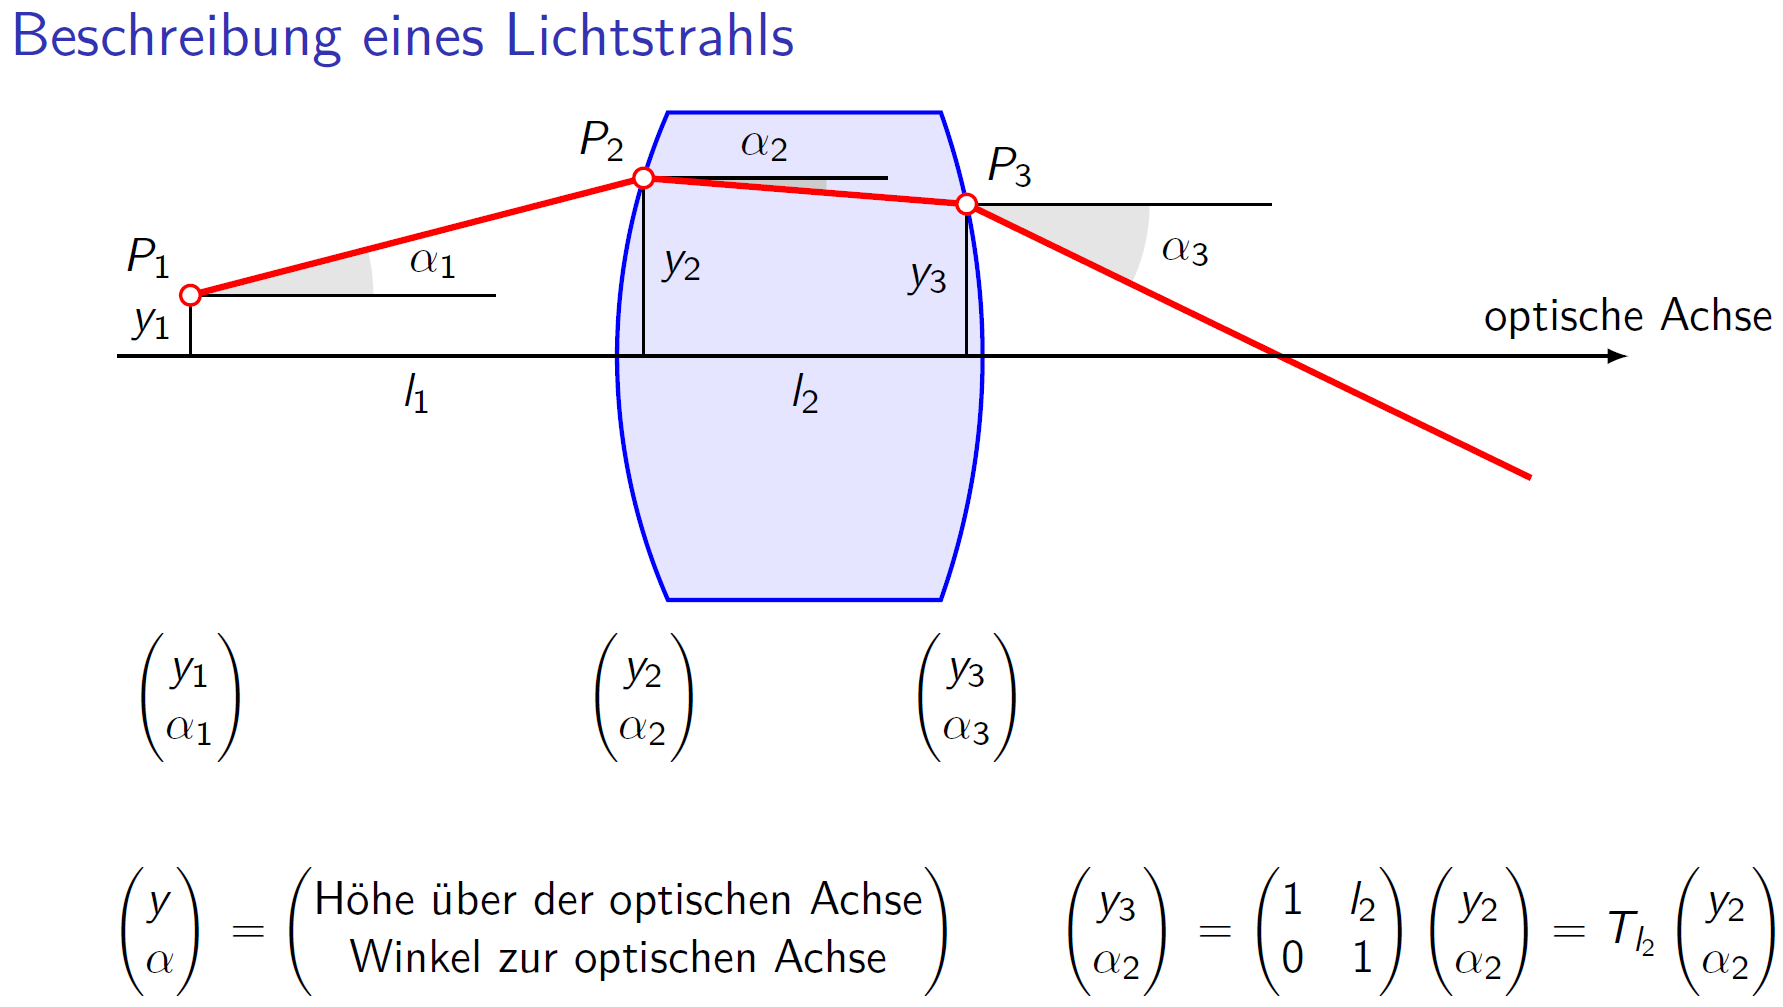
\includegraphics[width=0.85\linewidth]{Bilder/matrixoptik1} \\
		 
		 \vspace{0.5cm}
		 
		 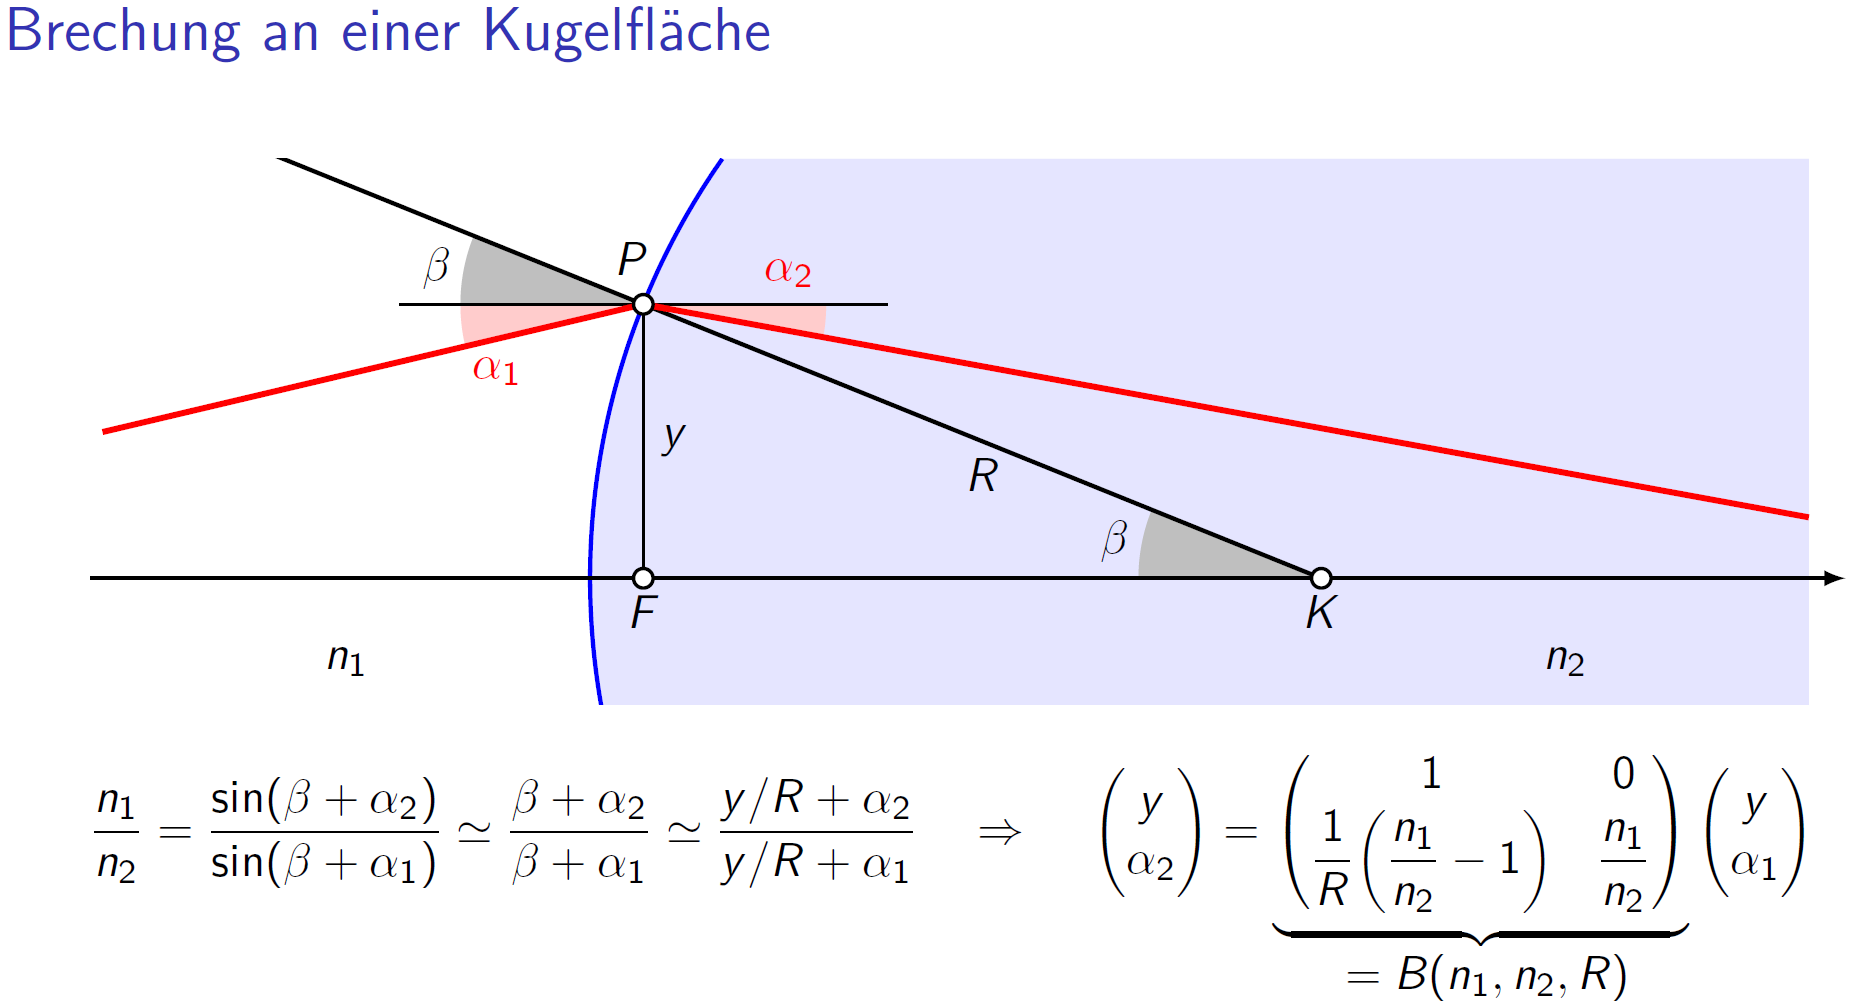
\includegraphics[width=0.85\linewidth]{Bilder/matrixoptik2} \\
		 
		 \vfill\null
		 \columnbreak
		 
		 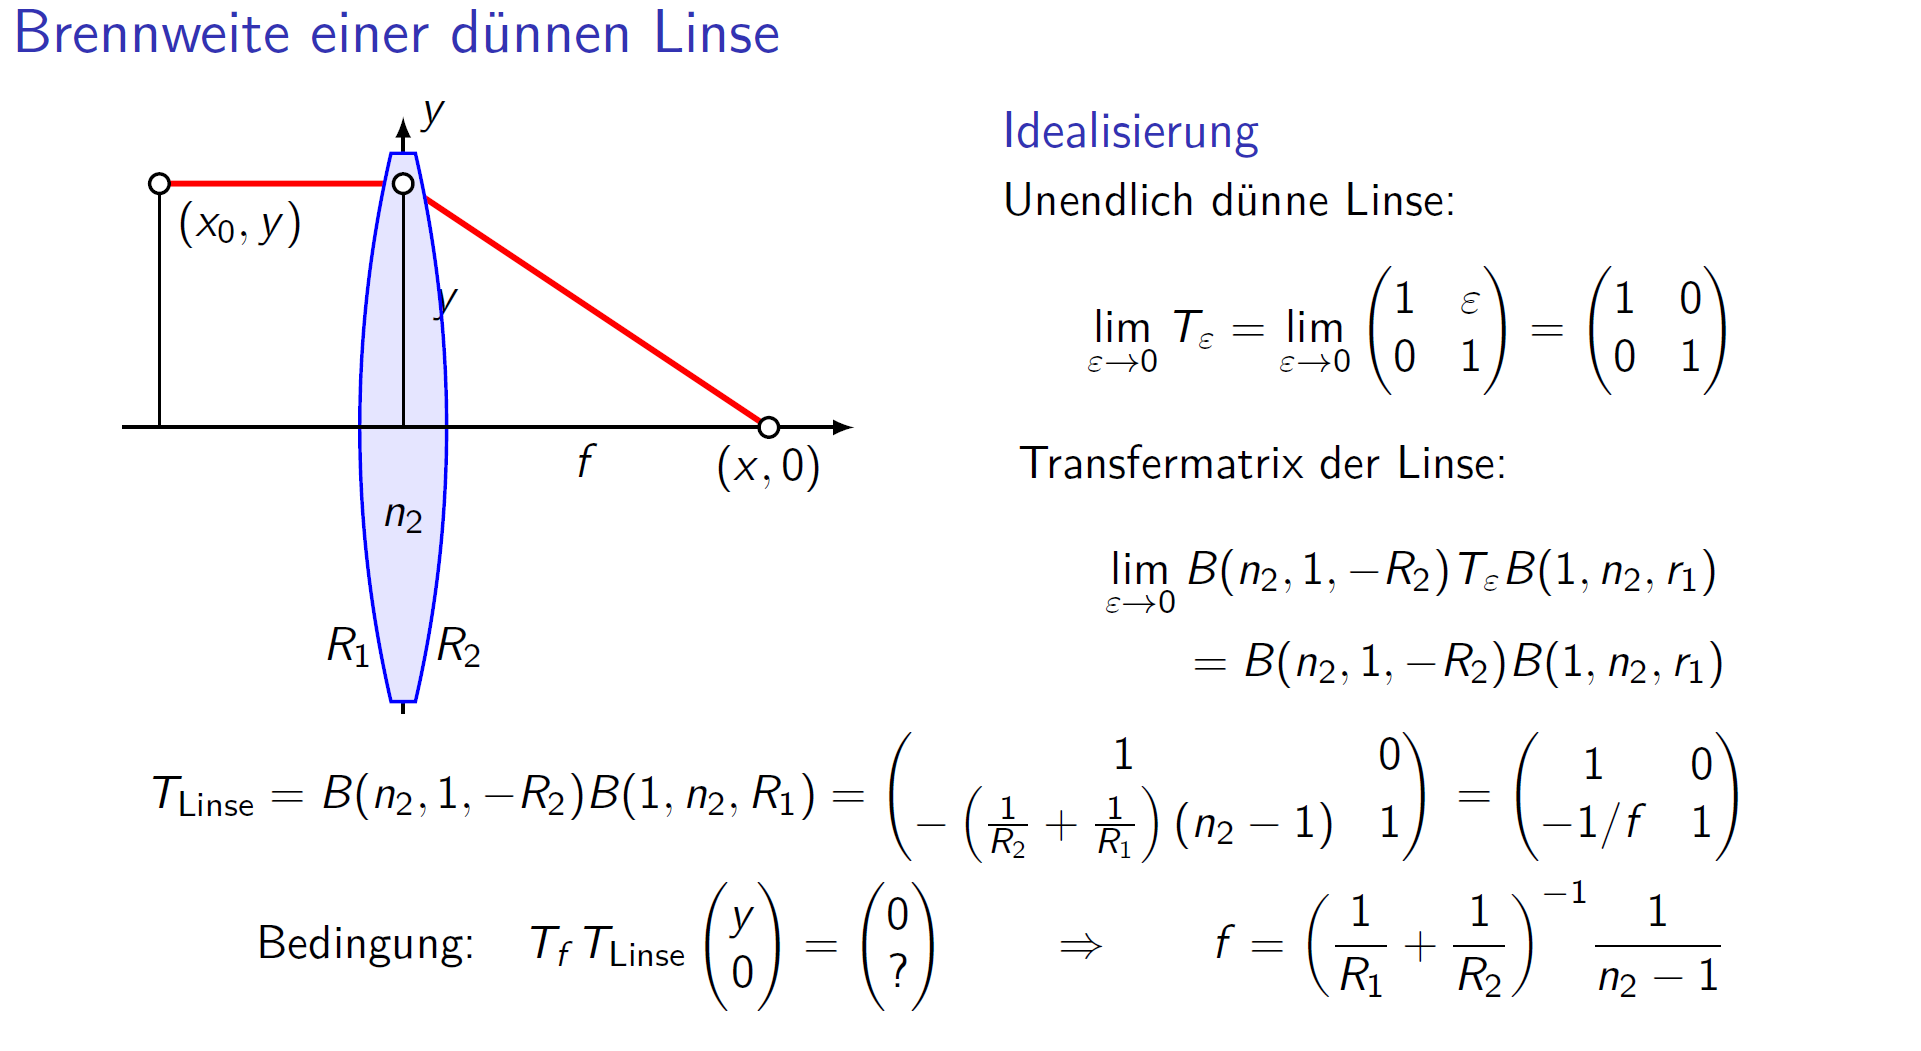
\includegraphics[width=0.8\linewidth]{Bilder/matrixoptik3} \\
		 
		 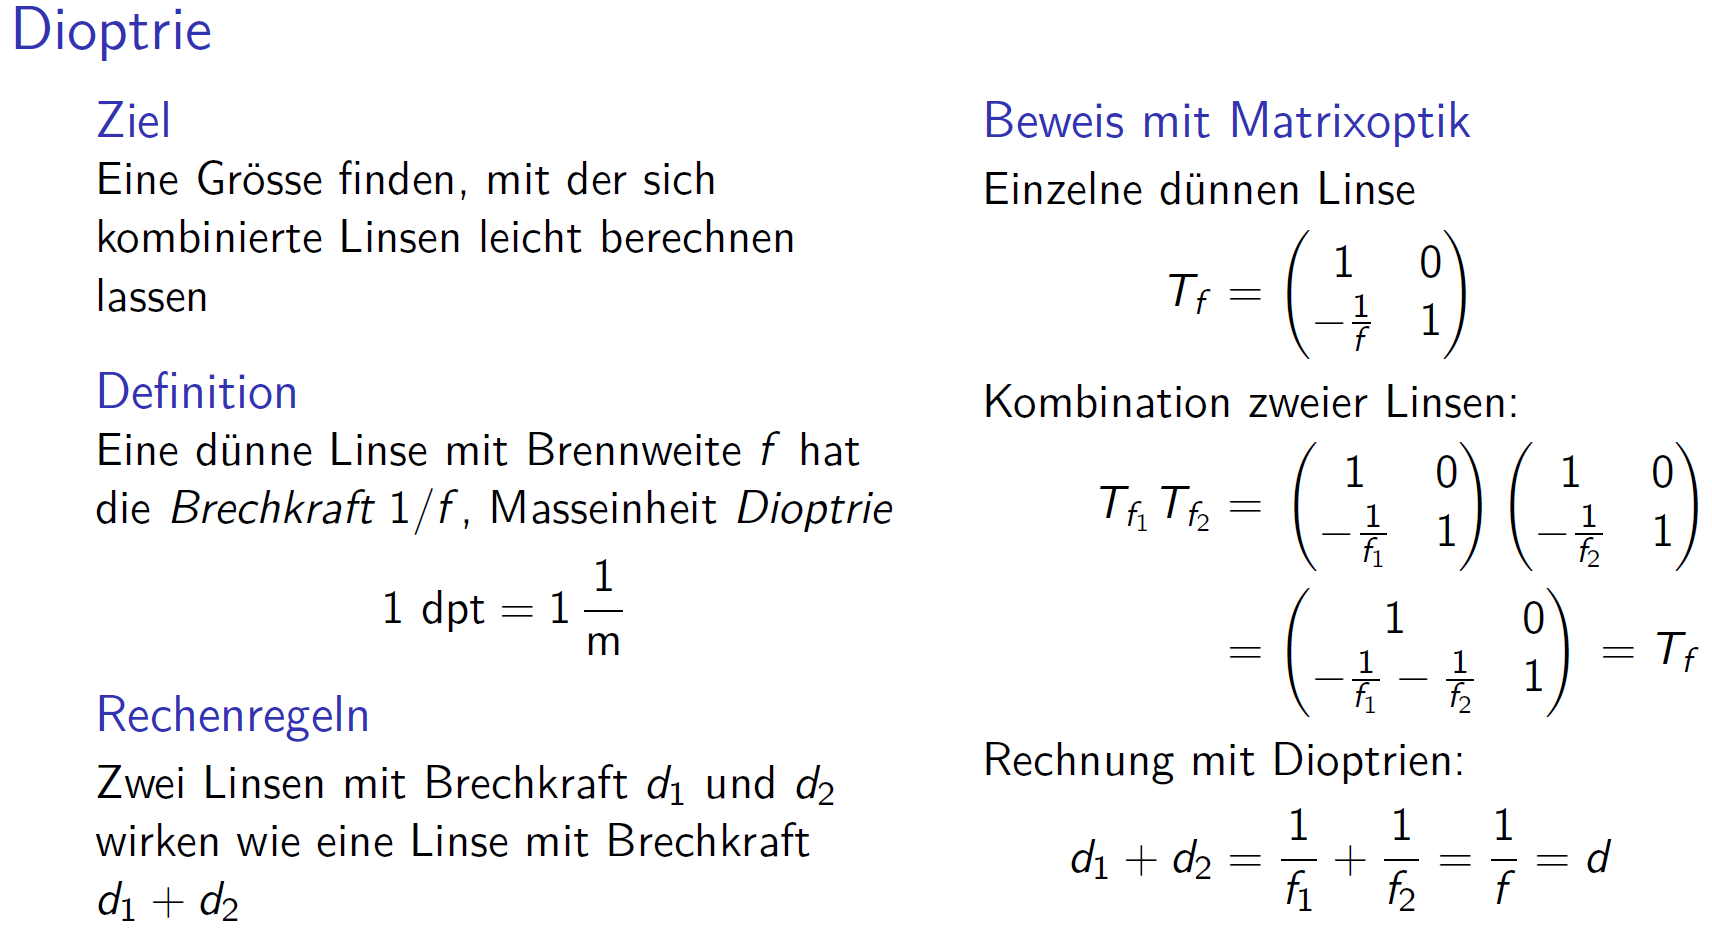
\includegraphics[width=0.8\linewidth]{Bilder/matrixoptik4} \\
		 
		 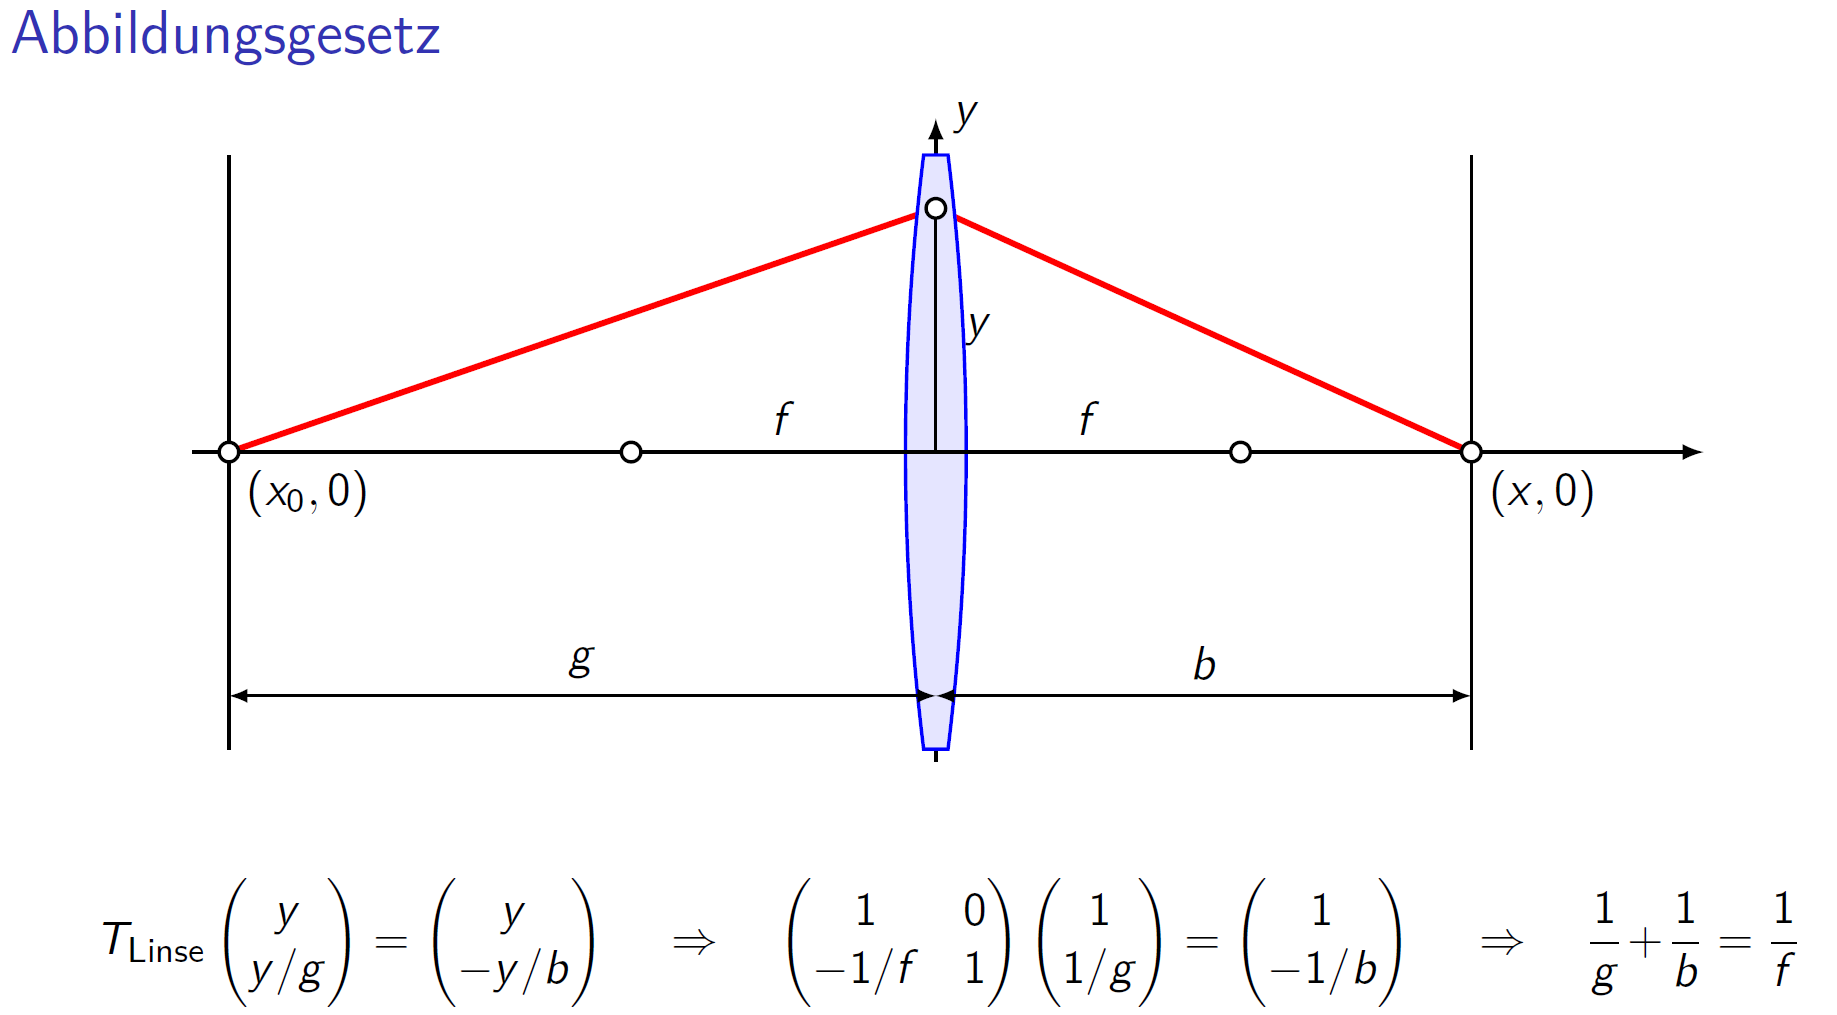
\includegraphics[width=0.8\linewidth]{Bilder/matrixoptik5}\\
		 
		 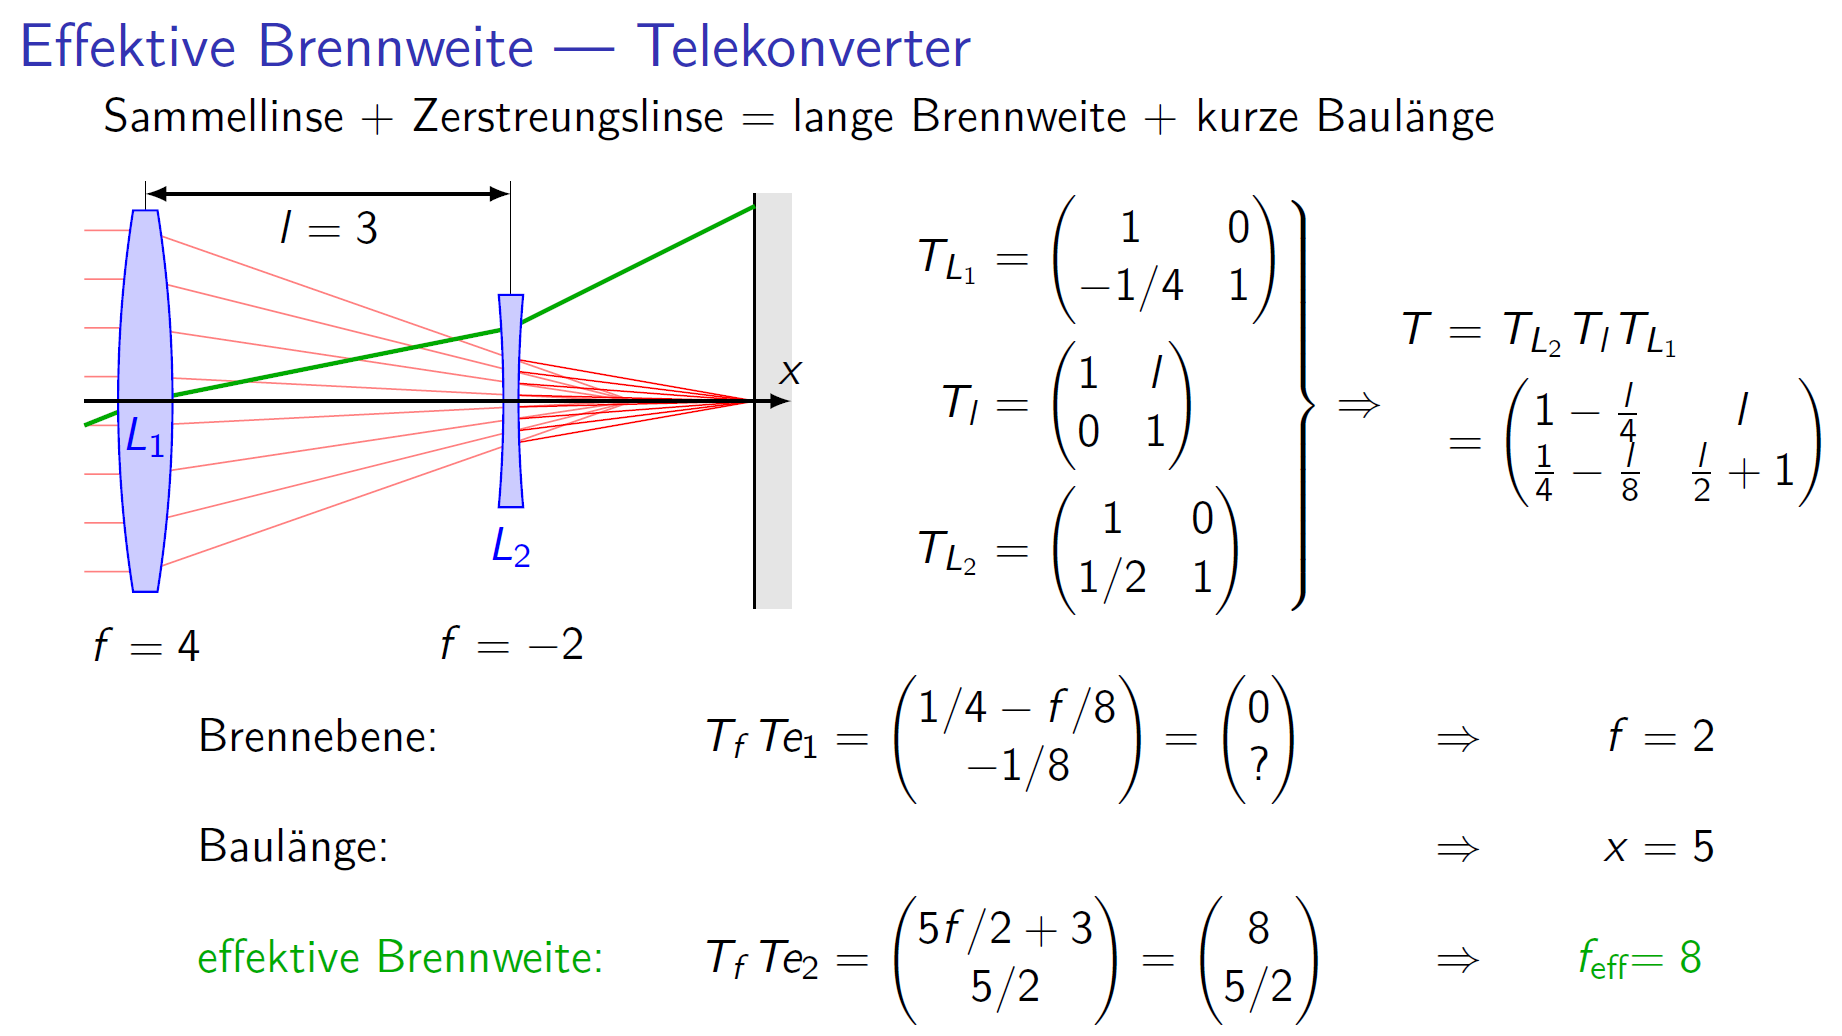
\includegraphics[width=0.8\linewidth]{Bilder/matrixoptik6} \\
		
		 
		 
		 \subsection{Kettenbrüche}
		 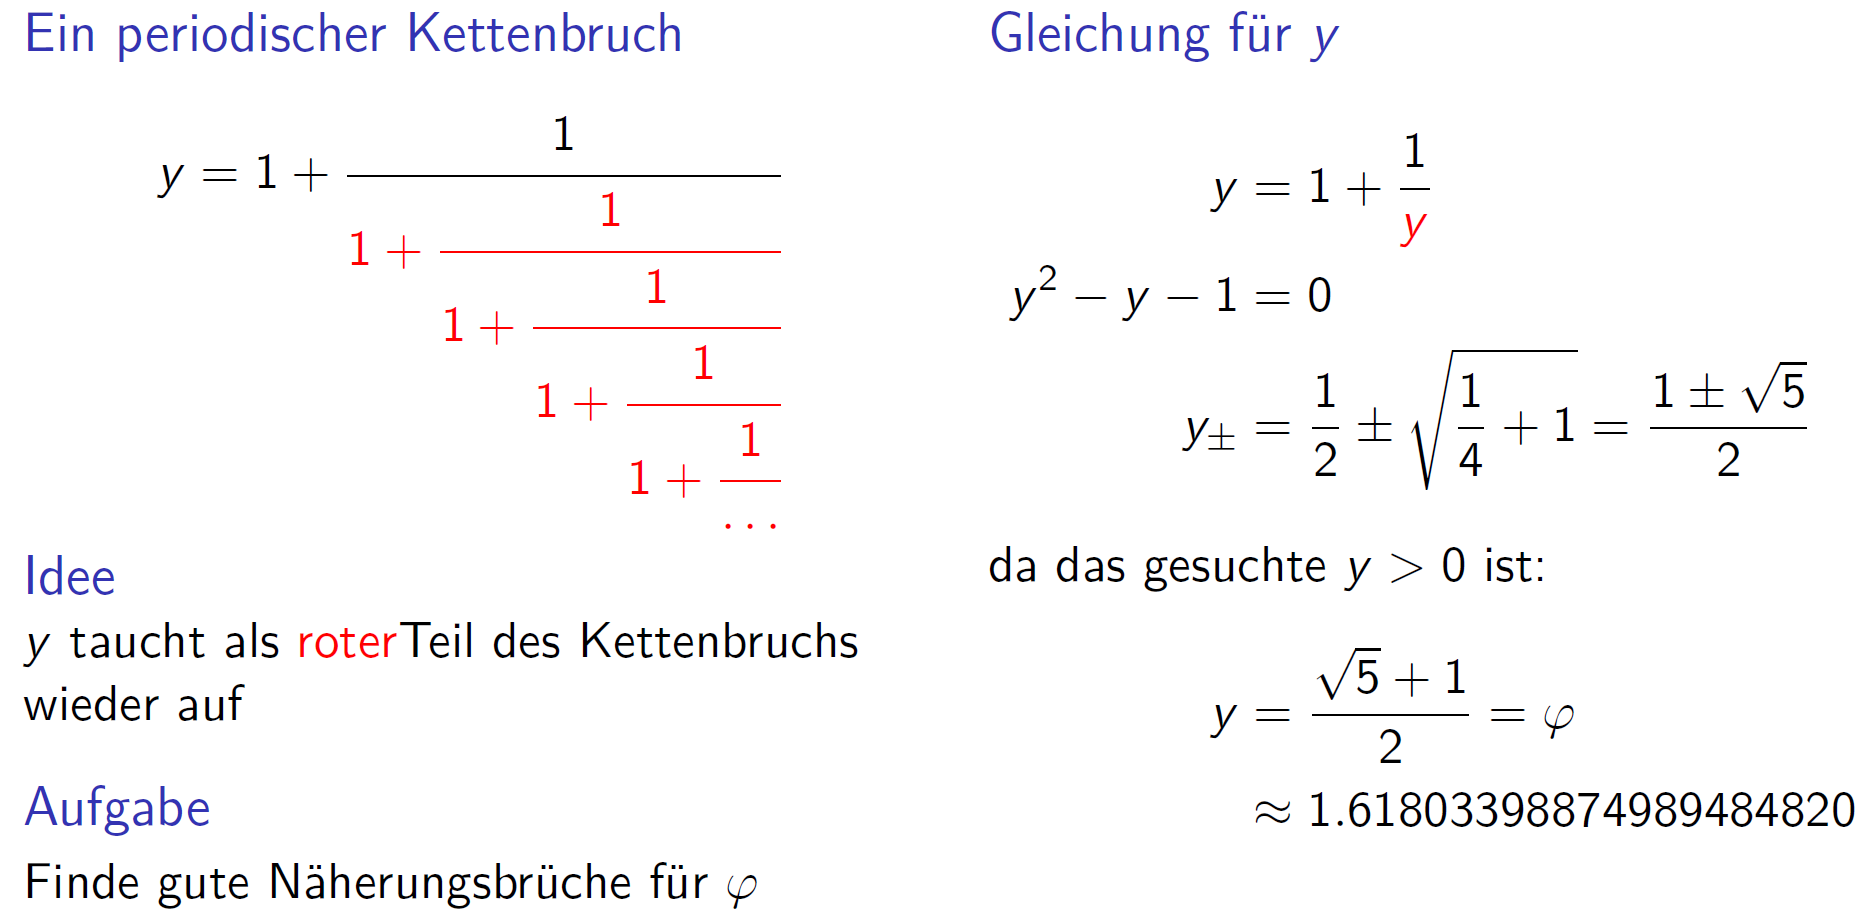
\includegraphics[width=0.8\linewidth]{Bilder/kettenbruch1} \\
		 
		 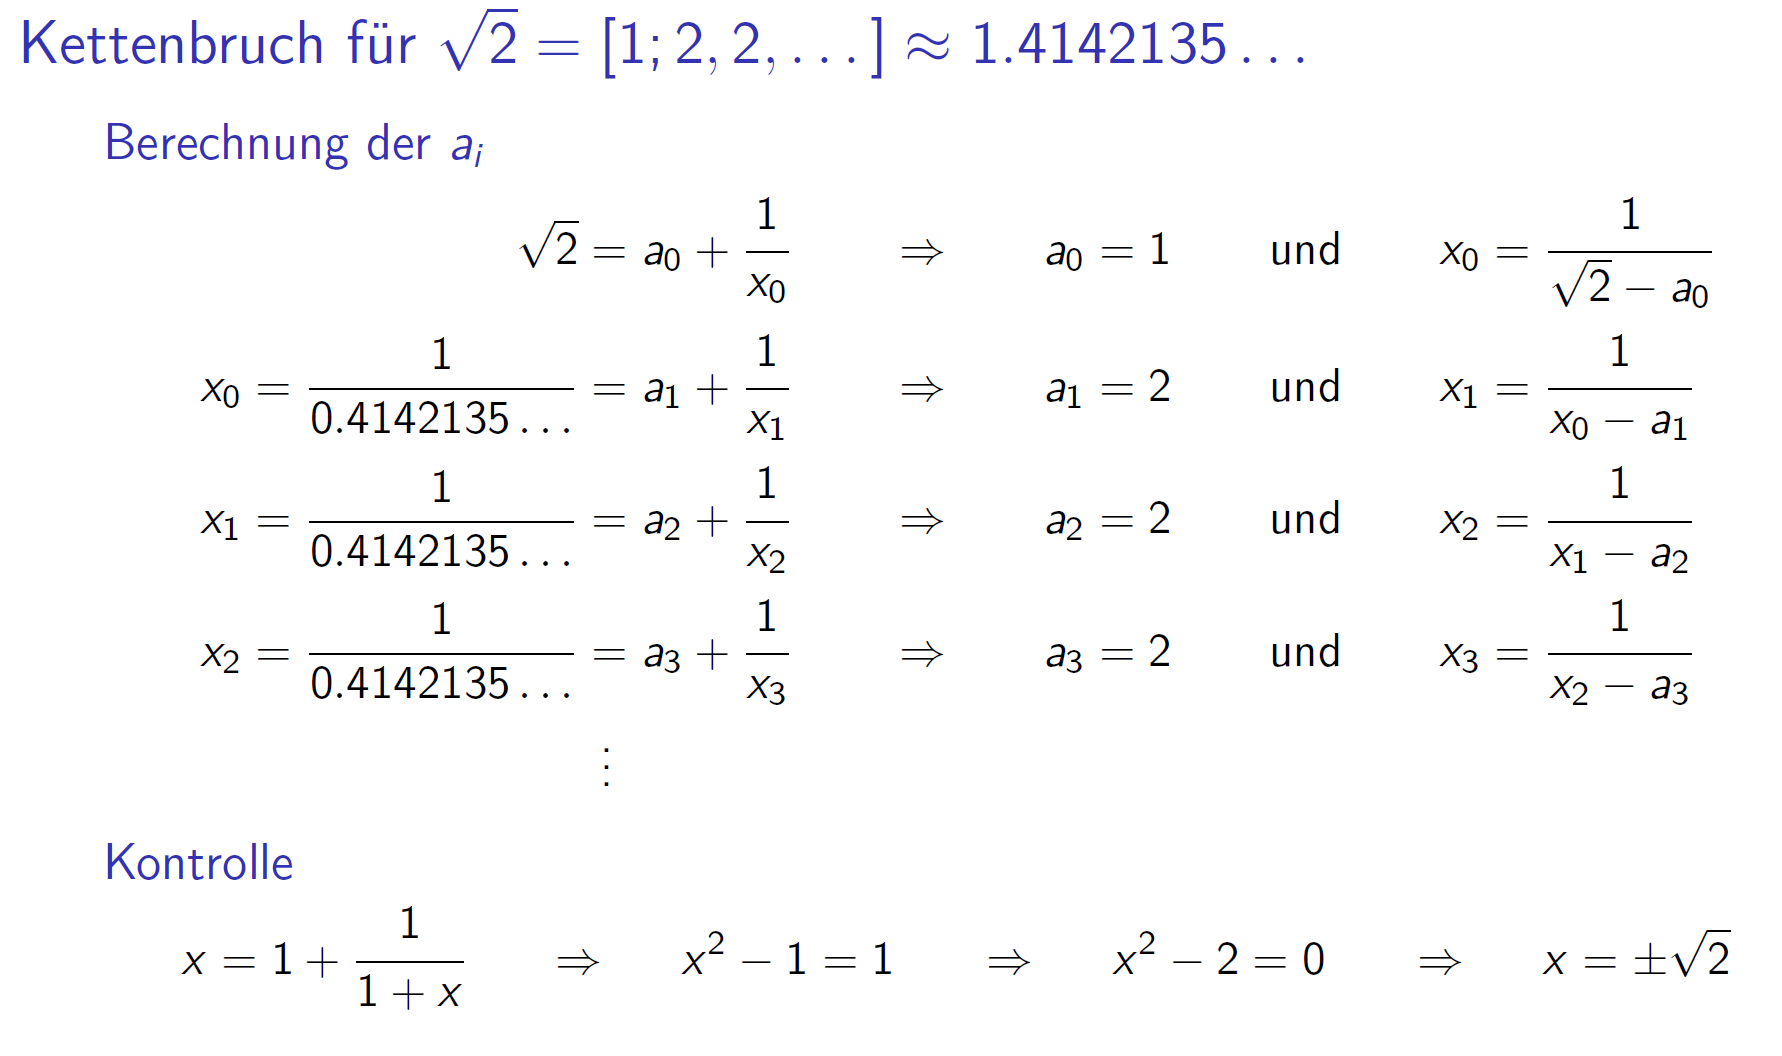
\includegraphics[width=0.8\linewidth]{Bilder/kettenbruch2} \\
		 
		 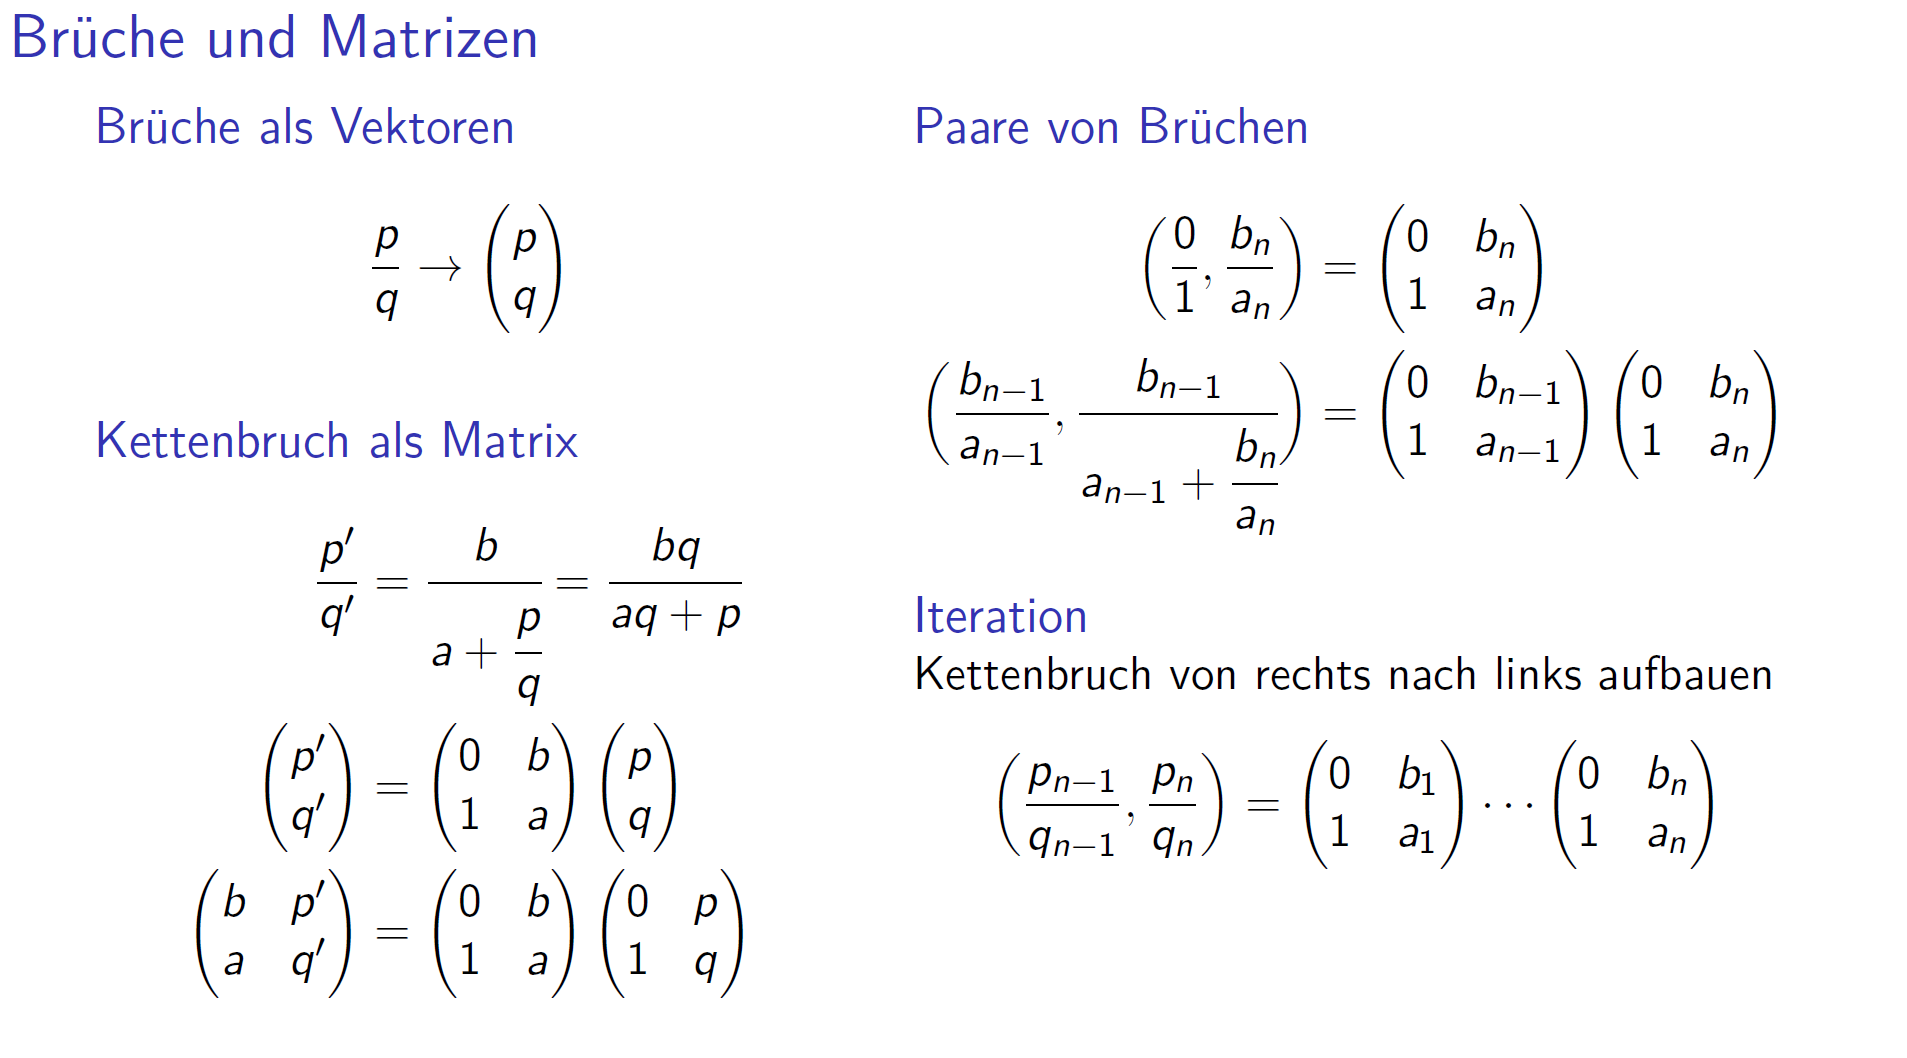
\includegraphics[width=0.8\linewidth]{Bilder/kettenbruch3} \\
		 
		 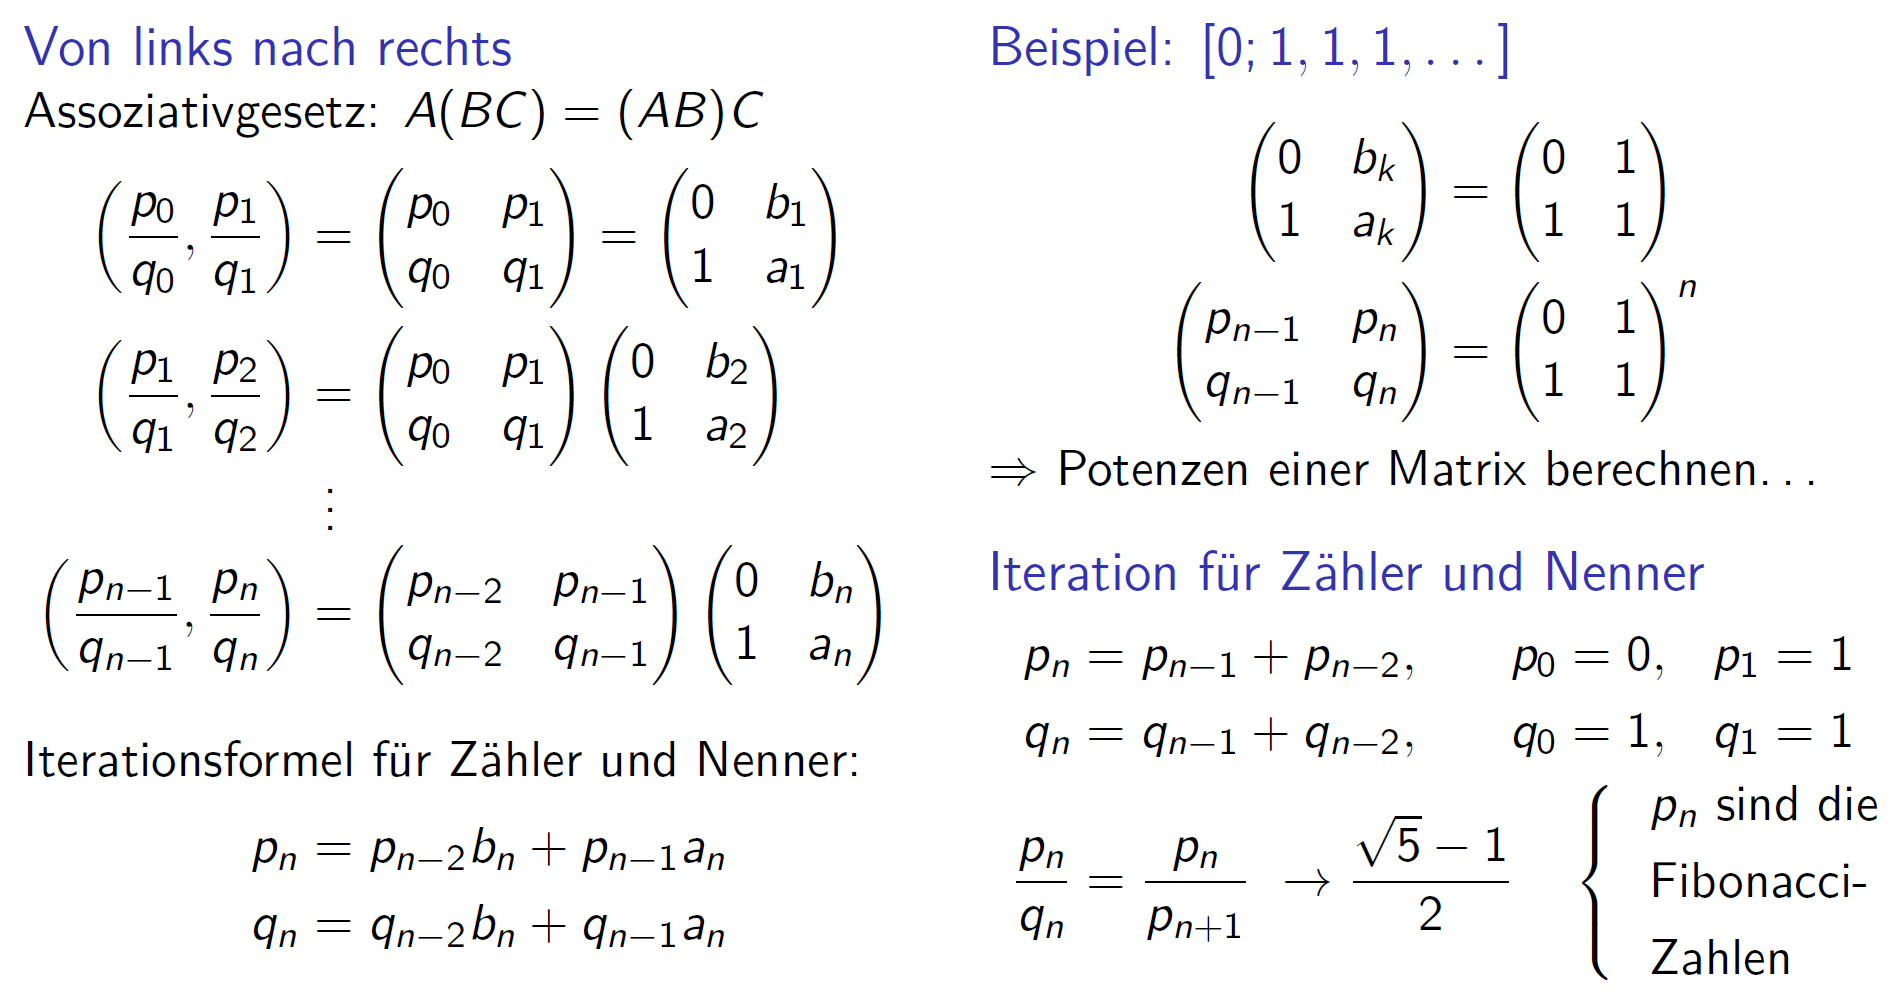
\includegraphics[width=0.8\linewidth]{Bilder/kettenbruch4} \\
		 
		 \includegraphics[width=0.8\linewidth]{Bilder/kettenbruch5} \\
		  
		 
		 
		 
		 \subsection{Rekursionsformeln}
		 \textbf{Anwendung Eigenwerte / Eigenvektoren / Eigenbasis} \\
		 \includegraphics[width=0.8\linewidth]{Bilder/rekursion1} \\ 
		 
		 
		 
		 
		\subsection{Kamerageometrie}		 
		 \includegraphics[width=0.9\linewidth]{Bilder/kamera1} \\
		 
		 \includegraphics[width=0.9\linewidth]{Bilder/kamera2} \\
		 
		 \includegraphics[width=0.9\linewidth]{Bilder/kamera3} \\
		 
		 \includegraphics[width=0.9\linewidth]{Bilder/kamera4} 	 
		 
		 
		 
		 
		 
		       
		    
		
		  \subsection{Widerstandsnetzwerk}
		   \includegraphics[width=0.8\linewidth]{Bilder/widerstand2} \\ 
		   
		   \includegraphics[width=0.8\linewidth]{Bilder/widerstand3} \\ 
		   
		   \includegraphics[width=0.8\linewidth]{Bilder/widerstand4} \\ 
		   
		   \includegraphics[width=0.8\linewidth]{Bilder/widerstand5} \\ 
		 
			    
	\end{multicols*}
\end{document}